% ------------------------------------------------------------------------
% Documento auxiliar (standalone) do TCC
% Segurança da comunicação dongle <-> servidor
%
% Compilar a partir deste diretório (latex/aux-docs):
%   latexmk -pdf segunraca-dongle-server.tex
% Reutiliza a bibliografia e as figuras do documento principal (../).
% ------------------------------------------------------------------------
\documentclass[
	12pt,
	article,			% documento curto: sem capítulos nem página de rosto
	oneside,
	a4paper,
	english,
	brazil				% o último idioma é o principal do documento
	]{abntex2}

% ---
% Pacotes básicos (mesmos do main.tex)
% ---
\usepackage{lmodern}
\usepackage[T1]{fontenc}
\usepackage[utf8]{inputenc}
\usepackage{indentfirst}
\usepackage{color}
\usepackage{graphicx}
\usepackage{microtype}
\usepackage{longtable}
\usepackage{tikz}
\usetikzlibrary{decorations.pathreplacing,arrows.meta,positioning,calc}
\usepackage{amsmath}
\usepackage{float}
\usepackage{array}

% Definição de cores para prioridades (mesmas do main.tex)
\definecolor{alta}{RGB}{200,0,0}
\definecolor{media}{RGB}{200,120,0}
\definecolor{baixa}{RGB}{0,140,0}

\newcommand{\palta}{\textcolor{alta}{\textbf{Alta}}}
\newcommand{\pmedia}{\textcolor{media}{\textbf{Média}}}
\newcommand{\pbaixa}{\textcolor{baixa}{\textbf{Baixa}}}

% ---
% Citações padrão ABNT
% ---
\usepackage[alf]{abntex2cite}

% Figuras do documento principal
\graphicspath{{../assets/}}

% ---
% Informações do documento
% ---
\titulo{Segurança da comunicação entre \textit{dongle} e servidor}

% ---
% Aparência do PDF
% ---
\definecolor{blue}{RGB}{41,5,195}
\makeatletter
\hypersetup{
	pdftitle={\@title},
	colorlinks=true,
	linkcolor=blue,
	citecolor=blue,
	filecolor=magenta,
	urlcolor=blue,
	bookmarksdepth=4
}
\makeatother

\begin{document}

\selectlanguage{brazil}
\frenchspacing

% Apenas o título (sem autor nem data)
\begin{center}
	{\Large\bfseries\imprimirtitulo\par}
\end{center}
\vspace{1em}

% ---
% Conteúdo
% ---
\textual

\section{Introdução} \label{sec:intro}

O propósito deste documento é modelar a implementação de uma comunicação com autenticidade entre
\textit{dongle} e um servidor externo, tendo como intermediário um \textit{app mobile} que se comunica com o 
\textit{dongle} por meio de \textit{BLE} e não pode ser confiado. Os dados devem trafegar 
para o servidor de modo que, ao recebê-los, deve ser criptograficamente garantido que eles foram 
medidos a partir do dongle que se identifica como originador do dado, a fim de que não seja 
possível alterar o conteúdo das medições ou deliberadamente esconder informação entre duas medições
diferentes sem que o servidor consiga detectar.

\section{Problemas a resolver} \label{sec:solucao}

O objetivo principal para o contexto deste trabalho é que as informações medidas pelo dongle que 
chegam no servidor possam ser confiadas e usadas para análises seguras a respeito do
funcionamento do carro e como ele está sendo conduzido. Assim, deve-se garantir autenticidade,
ou seja, todo registro recebido pelo servidor deve ter sido gerado pelo dongle associado a ele;
integridade, ou seja, o dado que é recebido pelo servidor não pode ter sido alterado; unicidade, 
ou seja, os registros devem ser recebidos uma única vez e a ordem em que eles foram gerados deve
ser mantida; e completude detectável, ou seja, o servidor deve saber exatamente se e quais registros
estão faltando ao sincronizar com o \textit{dongle}.

%e vínculo ao veículo, o que garante que o servidor consegue identificar quando há troca de veículo entre os \textit{boots} do dongle.

Nesse contexto, só é possível confiar plenamente no dongle e no servidor. Assim, o app e os enlaces BLE
e internet são modelados como não confiáveis, conforme a \autoref{fig:fronteiras-confianca}.

\begin{figure}[H]
	\centering
	\caption{Fronteiras de confiança entre \textit{dongle}, \textit{app} e servidor}
	\label{fig:fronteiras-confianca}
	% Fonte PlantUML: ../assets/aux-docs/plantuml/fronteiras-confianca.puml
	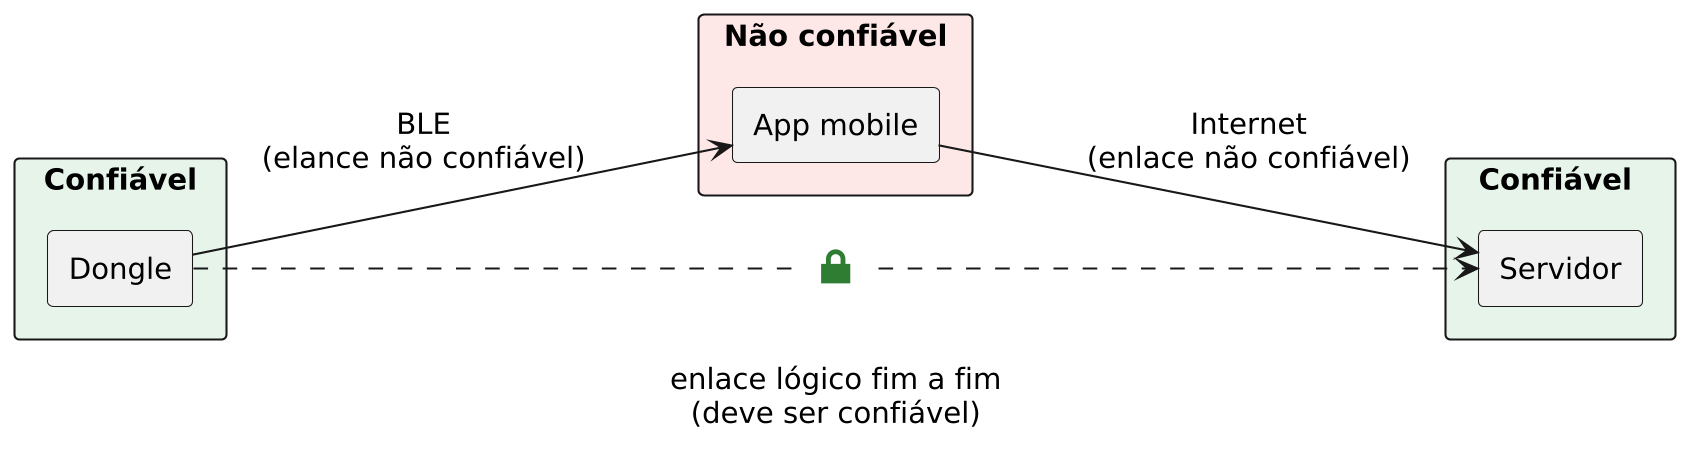
\includegraphics[width=\textwidth]{../../assets/aux-docs/fronteiras-confianca.png}
	\legend{Fonte: elaborado pelo autor.}
\end{figure}


\subsection{Modelagem de ataques}

Existem diversos adversários e ataques que podem ser modelados no cenário, envolvendo
os diferentes componentes e ligações entre eles. É possível dividir os ataques em três principais
categorias.

Dentro das categorias de ataque, também é possível definir cinco tipos principais de adversários que aparecem entre elas:

\begin{itemize}
    \item (AD1) o terceiro perto do carro que pode ter acesso ao enlace de rádio do BLE, cujo objetivo é espionar ou injetar dados;
    \item (AD2) o próprio motorista que tem acesso ao app original do sistema, cujo objetivo é esconder, alterar medidas do dongle ou enviar as medidas do dongle para terceiros não autorizados;
    \item (AD3) um app de terceiro no celular pareado que pode acessar as características BLE, cujo objetivo é coletar as informações medidas para outros propósitos;
    \item (AD4) um atacante na rede entre o celular e o servidor, cujo objetivo é ler ou alterar dados no caminho para o servidor;
    \item (AD5) um invasor no servidor que tem acesso ao banco de dados e tudo que está armazenado, cujo objetivo pode ser apagar ou forjar dados.
\end{itemize}


Para especificar os ataques, será utilizada uma metodologia de modelagem que define o adversário, a pré-condição do ataque, o método 
a partir do qual o ataque é executado, a vulnerabilidade que ele explora, o alvo que está sendo atacado, e, por fim, o efeito que o ataque causa.


\subsubsection{Comunicação wireless}  \label{secsec:comunicacao-wireless}

Esses são ataques que se concentram tanto no enlace BLE entre o app e dongle quanto na conexão de rede entre o app e o server. 
Dentre eles, estão sniffing, replay, Man In The Middle (MITM), acesso direto ao dongle por um terceiro e negação de serviço do enlace.

Abaixo estão modelados os ataques do ponto de vista do BLE, mas os mesmos princípios podem ser pensados para um adversário do tipo AD4 que interfere
na comunicação entre o app e o servidor.

Um exemplo de ataque dessa categoria é o sniffing (A1.1), no qual o adversário do tipo AD1 pode querer obter os dados do motorista, afetando sua
privacidade. A pré-condição é ter um sniffer ao alcance do sinal do BLE, cujo enlace não é cifrado. O método a partir do qual ele é feito é
seguir a conexão e recuperar tudo que passa pelas características do dongle de maneira passiva. A vulnerabilidade explorada é a falta de cifração
nas características BLE, o alvo são os dados transferidos pelo enlace, e o efeito é o vazamento de dados medidos pelo dongle.

No ataque de \textit{replay} (A1.2), o adversário do tipo AD1 quer repetir comandos ou respostas para alterar o estado do dongle ou enganar o app.
A pré-condição é ter capturado o tráfego por \textit{sniffing} e conseguir se conectar ao dongle ou se passar por ele. O método consiste em
reescrever na característica de recepção quadros gravados anteriormente, como \texttt{AT\#DIAG 1}, \texttt{AT\#PID} ou \texttt{ATZ}, ou em se
anunciar como o dongle e devolver respostas antigas ao app. A vulnerabilidade explorada é a ausência de autenticação da conexão e de
garantia de frescor das mensagens, somada ao fato de o app não verificar a identidade do dongle. O alvo são o modo e a configuração do dongle
e os dados exibidos pelo app, e o efeito é uma coleta pausada ou reconfigurada sem o conhecimento do motorista, ou um painel com valores falsos.

Já no \textit{Man In The Middle} (A1.3), o adversário do tipo AD1 quer ler e alterar em tempo real o que app e dongle trocam. A pré-condição é estar
presente quando o app se conecta ou durante o pareamento, com dois rádios BLE. O método é conectar-se ao dongle, anunciar um clone dele ao
app e repassar todo o tráfego entre os dois, alterando valores ou inserindo comandos no caminho. A vulnerabilidade explorada é que nenhum dos
lados autentica o outro no enlace, o alvo é a integridade de comandos e respostas, incluindo as requisições ao barramento CAN no modo
diagnóstico, e o efeito é um painel adulterado e requisições injetadas no carro.

Por fim, no acesso direto (A1.4), o adversário do tipo AD1 quer usar o dongle como se fosse o app. A pré-condição é que o dongle aceite conexões
de qualquer dispositivo, e o método é simplesmente conectar-se e escrever comandos na característica de recepção, inclusive requisições ao
barramento CAN no modo diagnóstico. A vulnerabilidade explorada é a falta de autenticação da conexão, agravada pelo dongle aceitar uma
segunda conexão simultânea. O alvo são os dados medidos, o modo diagnóstico e a configuração do dongle, e o efeito é a leitura dos dados,
a pausa da coleta e consultas ao veículo feitas em nome do dono.

Na negação de serviço do enlace (A1.5), o adversário do tipo AD1 quer impedir que o app se comunique com o dongle, atacando a
disponibilidade da conexão. A pré-condição é estar ao alcance do sinal BLE do dongle. O método é conectar-se ao dongle assim que ele
começa a se anunciar e manter a conexão aberta, ocupando as conexões que ele aceita, de modo que o app oficial não consiga se conectar. 
A vulnerabilidade explorada é que o dongle aceita conexões de qualquer dispositivo e tem um número limitado delas. O alvo é a disponibilidade 
do enlace BLE e, por consequência, a sincronização dos registros com o servidor, e o efeito é um dongle inacessível ao app: o painel deixa de 
ser atualizado e o servidor recebe um intervalo sem dados que não é causado pelo motorista.

\subsubsection{Comunicação entre carro e dongle} \label{secsec:comunicacao-carro-dongle}

Já esses ataques acontecem no barramento CAN entre o carro e o dongle, ou seja, o atacante pode
usar algum elemento externo para simular a CAN do veículo por inteiro ou para sobrescrever um determinado PID a fim de
manipular leituras.

No ataque de ECU emulada (A2.1), o adversário do tipo AD2 quer que a seguradora receba uma condução melhor do que a real. A pré-condição é ter
acesso físico à porta OBD e um emulador ou \textit{gateway} CAN, sendo que o próprio ECUSim deste projeto serve como prova de conceito.
O método é ligar o dongle no emulador, ou colocar um \textit{gateway} entre a porta e o dongle que repassa as requisições ao carro e altera
apenas as respostas escolhidas, como limitar a velocidade reportada. A vulnerabilidade explorada é que as respostas OBD-II não são
autenticadas, de modo que o dongle confia em quem responder. O alvo é a veracidade dos dados medidos antes de serem assinados, e o efeito
são registros autênticos com conteúdo falso: a assinatura prova que o dongle mediu, mas não que o carro disse aquilo.

Na resposta concorrente no barramento (A2.2), o adversário do tipo AD2 quer sobrescrever apenas alguns PIDs sem retirar o carro do barramento.
A pré-condição é ter um dispositivo ligado ao CAN capaz de responder mais rápido que a ECU. O método é escutar as requisições funcionais,
enviadas para o identificador 0x7DF, e responder em 0x7E8 antes da ECU real. A vulnerabilidade explorada é a mesma do ataque anterior,
somada ao fato de o dongle aceitar a primeira resposta da faixa 0x7E8--0x7EF sem endereçar ECUs específicas. O alvo é a veracidade dos PIDs
escolhidos, e o efeito, além dos registros autênticos com conteúdo falso, é um painel e um diagnóstico enganados.

\subsubsection{App malicioso} \label{secsec:app-malicioso}

Como o aplicativo será instalado no aparelho do usuário do dongle, um aparelho com \textit{root} tem total controle do
funcionamento do app e pode manipulá-lo para gerar ataques ao sistema. Esses ataques podem manipular o processo de envio dos
dados entre o app e o servidor a fim de fazer com que as informações do servidor não correspondam com o que foi realmente medido 
pelo dongle no carro. O principal adversário nesse contexto é o do tipo AD2, que controla o app e pode querer forjar cenários de
medição que vão de encontro aos interesses da entidade no servidor externo, como uma seguradora ou gerenciadora de frotas.

Na exfiltração (A3.1), o adversário do tipo AD3, ou um SDK de terceiros embutido no próprio app, quer vender ou usar para outros fins os dados de
condução e de posição do motorista. A pré-condição é ter permissão de Bluetooth e de internet no celular pareado com o dongle. O método é
conectar-se ao dongle quando o app oficial não está conectado e ler os dados medidos, ou ler os registros e posições que passam pelo app,
enviando tudo a outro servidor. A vulnerabilidade explorada é que os dados não são cifrados na camada de aplicação e que a autorização é
feita por aparelho, e não por app. O alvo é a privacidade do motorista, e o efeito é o vazamento de dados pessoais e o rastreamento do veículo.

Já na omissão de mensagens do servidor (A3.2), o adversário do tipo AD2, por meio de um app modificado, quer degradar a coleta sem que a culpa
recaia sobre o app. A pré-condição é que o app seja o único caminho entre o servidor e o dongle. O método é receber do servidor o desafio, a
confirmação de recebimento ou o \textit{token} de diagnóstico e não repassá-los ao dongle, ou repassar apenas alguns. A vulnerabilidade
explorada é que as mensagens do servidor não têm confirmação de entrega ao dongle. O alvo é a recuperabilidade dos registros, a âncora de
tempo e a troca de época, e o efeito é que, sem confirmações, a memória do dongle enche e ele descarta registros antigos; sem desafio, não
há âncora de tempo nem época nova; e, sem \textit{token}, o diagnóstico é negado.

Na alteração de medições (A3.3), o adversário do tipo AD2 quer melhorar o próprio histórico. A pré-condição é controlar o app, ou um \textit{proxy}
com uma autoridade certificadora instalada no celular, e o método é modificar bytes de um bloco antes de enviá-lo ao servidor. A
vulnerabilidade explorada é a ausência de integridade fim a fim, o alvo é a integridade dos registros, e o efeito é a aceitação de dados falsos.

Na repetição de medições (A3.4), o adversário do tipo AD2 quer repetir uma viagem tranquila. A pré-condição é ter gravado blocos antigos, e o método
é reenviar ao servidor blocos já aceitos. A vulnerabilidade explorada é a falta de garantia de unicidade, o alvo é a unicidade dos registros,
e o efeito são dados duplicados no servidor.

Na reordenação das medidas enviadas (A3.5), o adversário do tipo AD2 quer deslocar eventos no tempo. A pré-condição é controlar o app, e o método é enviar os blocos
fora de ordem. A vulnerabilidade explorada é que a ordem dos registros não é garantida, o alvo é a ordem dos registros, e o efeito é uma
linha do tempo falsa.

No descarte de medições intermediárias (A3.6), o adversário do tipo AD2 quer apagar um evento específico, como uma frenagem brusca. A pré-condição
é controlar o app, e o método é deixar de enviar os blocos escolhidos. A vulnerabilidade explorada é a falta de completude, o alvo é a
completude dos registros, e o efeito é uma lacuna silenciosa nos dados do servidor.

Ao omitir as últimas medições (A3.7), o adversário do tipo AD2 quer omitir a última viagem. A pré-condição é controlar o app, e o método é parar de enviar
blocos antes do último. A vulnerabilidade explorada é que o servidor não conhece o número de sequência do último registro gerado, o alvo é a
completude dos registros, e o efeito é uma perda de dados invisível ao servidor.

\subsection{Definição de escopo e mitigação de ataques}


Tendo em vista todos esses possíveis ataques, é necessário alinhar o escopo do projeto de acordo com o objetivo que ele se propõe a cumprir.
Como a ideia é fazer com que os dados cheguem no servidor de maneira confiável e completa, foram priorizados os ataques da categoria \ref{secsec:app-malicioso},
sendo o objetivo deste documento explicar em detalhe um protocolo que garante, nesse cenário de desconfiança no canal e no aplicativo que intermedia o envio dos dados,
como garantir autenticidade, integridade, unicidade e completude detectável dos dados medidos pelo dongle.

Além disso, para complementar a segurança da comunicação fim a fim, também será abordado o uso de segurança entre os enlaces BLE e internet para abordar os ataques 
modelados na seção \ref{secsec:comunicacao-wireless}. Como já existem protocolos estabelecidos para garantir essa segurança, a ideia é usá-los para garantir
confidencialidade na comunicação: para o enlace entre o dongle e o app, será utilizada a técnica LESC (LE Secure Connections) do BLE; já para o enlace entre app e servidor
será utilizado o protocolo HTTPS/TLS, que é amplamente utilizado para garantir a segurança de comunicação entre clientes e servidores na internet.

Fica como limitação do projeto a mitigação de ataques que envolvam o barramento CAN do veículo, como os da categoria \ref{secsec:comunicacao-carro-dongle},
pois o escopo do projeto envolve apenas os dados medidos pelo dongle, sem abordar a garantia de que o dongle está realmente conectado em uma rede CAN válida, o
que deve ser garantido externamente. Alguns exemplos de mitigação para isso são incorporar o dongle dentro da arquitetura do carro e não exposto na conexão OBD2 interna,
configurar alertas de desconexão para entender se o dongle foi retirado a fim de ser colocado em um simulador, ou cruzar a medida com sensores externos de velocidade e 
localização instalados externamente à rede CAN.

\section{Segurança na comunicação sem fio}

\subsection{BLE LESC}

O LE Secure Connections (LESC) é um método de pareamento introduzido no Bluetooth 4.2 para substituir o esquema de chave temporária de baixa entropia no pareamento legado
do BLE, que era facilmente quebrada por força bruta. Para isso, o LESC estabelece a chave do enlace com uma troca de chaves Diffie-Hellman em curva elíptica (ECDH)
na curva P-256. Com essa chave de enlace, cada um dos aparelhos deriva uma chave de sessão com a qual o enlace é cifrado e autenticado usando AES-CCM, o que garante 
confidencialidade e integridade na comunicação. Quando os dois aparelhos são pareados, ou seja, geram a chave de enlace válida, é feito o \textit{bonding}: a chave de sessão
é salva em cada um dos aparelhos para futuras conexões, de modo que não seja necessário repetir o processo de pareamento.

Esse pareamento é feito com um total de 3 fases. Na primeira fase, os aparelhos declaram suas capacidades e requisitos de autenticação como, por exemplo, se têm capacidade
de entrada e saída e se suportam LESC. Trocadas as capacidades, os dispositivos decidem se continuam o pareamento e é escolhido um método de associação, os quais estão especificados
na tabela \ref{lesc:metodos}, na qual considera-se implícita a pré-condição de que ambos os lados suportam LESC.

\begin{table}[H] 	\label{lesc:metodos}
	\centering
	\caption{Métodos de associação do LESC}
	\begin{tabular}{|>{\centering\arraybackslash}m{0.2\textwidth}|>{\raggedright\arraybackslash}m{0.25\textwidth}|>{\raggedright\arraybackslash}m{0.45\textwidth}|}
		\hline
		\textbf{Método} & \textbf{Pré-condição} & \textbf{Descrição} \\
		\hline
		Just Works & - & Não há autenticação do outro lado, apenas a troca de chaves ECDH. Vulnerável a MITM. \\
		\hline
		Numeric Comparison & Ambos têm display e entrada & Um número é gerado e exibido em ambos os lados, que devem confirmar se são iguais. \\
		\hline
		Passkey Entry & Um tem display e outro tem entrada & Um lado gera um número de 6 dígitos e o outro deve digitá-lo. \\
		\hline
		OOB \newline (Out of Band) & Canal seguro externo entre os dispositivos & Dados de autenticação são trocados por um canal seguro externo, como NFC. \\
		\hline
	\end{tabular}
\end{table}

\subsection{HTTPS/TLS}

O mesmo problema de confidencialidade e integridade de comunicação sem fio que é identificado entre o dongle e o app, também pode ser identificado quando o app
vai se comunicar com o servidor: deve haver confidencialidade, autenticidade e integridade na troca de pacotes pela rede. Para isso, o servidor deve ter um certificado
TLS válido a fim de que seja possível estabelecer uma troca de chaves com autenticidade. Em seguida, com a chave estabelecida, há garantia de integridade, confidencialidade
e autenticidade entre a conexão app e servidor.

\section{Segurança na comunicação fim a fim}

Esta seção tem como propósito modelar como deve ser feita a comunicação fim a fim, entre dongle e servidor, garantindo que haja todas as propriedades de segurança previstas
no projeto. A ideia é comparar com benchmarks duas implementações diferentes: usando MAC (Message Authentication Code) com chave simétrica pré-compartilhada (PSK) e usando 
assinatura digital via chave assimétrica. Em ambas as formas, a ideia é o dongle conseguir provar criptograficamente que validou os blocos antes de enviá-los para o servidor e,
quando esses blocos chegarem no seu destino, o servidor consiga validar que os blocos que chegaram pela rede são de fato gerados pelo dongle. 

Para entender a necessidade dessa modelagem, é importante deixar claro o motivo das camadas de LESC e HTTPS na comunicação não serem suficientes. Esses dois mecanismos garantem
segurança na comunicação entre dongle e app e entre app e servidor, respectivamente, mas não conseguem garantir que pacotes realmente foram gerados pelo dongle, uma vez que eles
serão transmitidos por meio de um intermediário que tem controle total sobre o conteúdo.

\subsection{Geração de chaves e identificação do dongle}

Na fabricação do dongle, serão gerados um \textit{DevId} de 8 bytes e duas chaves $K_{auth}$ e $K_{rec}$ de 32 bytes cada. Cada um desses elementos é sorteado usando forte
entropia ao fabricar o dongle. As chaves são gravadas na NVS do dongle e registradas em um serviço de KMS (Key Management System) em um servidor separado ($S_{KMS}$), 
trafegando na rede criptografadas com uma chave pública fornecida por $S_{KMS}$; dessa maneira, a chave fica em claro apenas por pouco tempo na memória da estação
de fabricação.

O uso de um KMS é importante pois permite que o servidor consiga verificar e gerar MACs sem que a chave precise estar na memória do servidor de aplicação ($S_{App}$), que
é um alvo de mais fácil acesso e, portanto, com maior risco de comprometimento, diminuindo a superfície de ataque para adversários do tipo AD5. Ainda há superfície de ataque
no servidor do KMS, mas ele não é exposto à internet e pode ter um controle de acesso bem mais rígido. 

A escolha de usar duas chaves é para que $K_{auth}$ seja usada para criar MAC nas mensagens de autenticação entre o servidor e o dongle, enquanto $K_{rec}$ fica apenas para
gerar MAC dos blocos de dados que saem do dongle até o servidor. Assim, é possível gerenciar as permissões do KMS para que o servidor de aplicação consiga gerar e verificar
MACs com $K_{auth}$, mas consiga apenas verificar MACs com $K_{rec}$. Assim, mesmo que $S_{App}$ seja comprometido, um atacante não consegue gerar MACs válidos para um dongle
sem também comprometer o $S_{KMS}$.

Enquanto do lado do servidor o KMS garante a proteção das chaves, o dongle conta com o armazenamento das chaves no NVS (Non-Volatile Storage) com encriptação. Para garantir maior segurança
dessa encriptação, também conta com: Secure Boot V2 para rodar apenas \textit{firmware} assinado e não permitir injeção arbitrária de código; \textit{flash encryption} para cifrar as partições
da flash e a chave de encriptação do NVS; \textit{eFuse}, memória gravável e não editável que guarda configurações da placa como o bloqueio do uso de JTAG e download pela UART, evitando depuração, 
e também guardar a chave de encriptação da flash, contando com bloqueio total de leitura. Mesmo com todas essas camadas de proteção, ainda há risco de ataques com atacantes extremamente qualificados.

Uma evolução para guardar melhor as chaves é o uso de um elemento seguro de hardware, como o chip ATECC608B, para armazenar as chaves fora da ESP. Como, embora muito mais difícil,
ainda é possível extrair chaves de elementos seguros, não vale a pena o seu uso dentro desse projeto, pois agrega apenas em aumento de custo para um ataque de recuperação de chave e não configura uma
melhoria academicamente relevante em relação à segurança dentro do escopo deste trabalho.

\begin{figure}[H]
	\centering
	\caption{Interação entre o app, o servidor de aplicação e o servidor KMS}
	\label{fig:kms-servidor-app}
	% Fonte PlantUML: ../assets/aux-docs/plantuml/kms-servidor-app.puml
	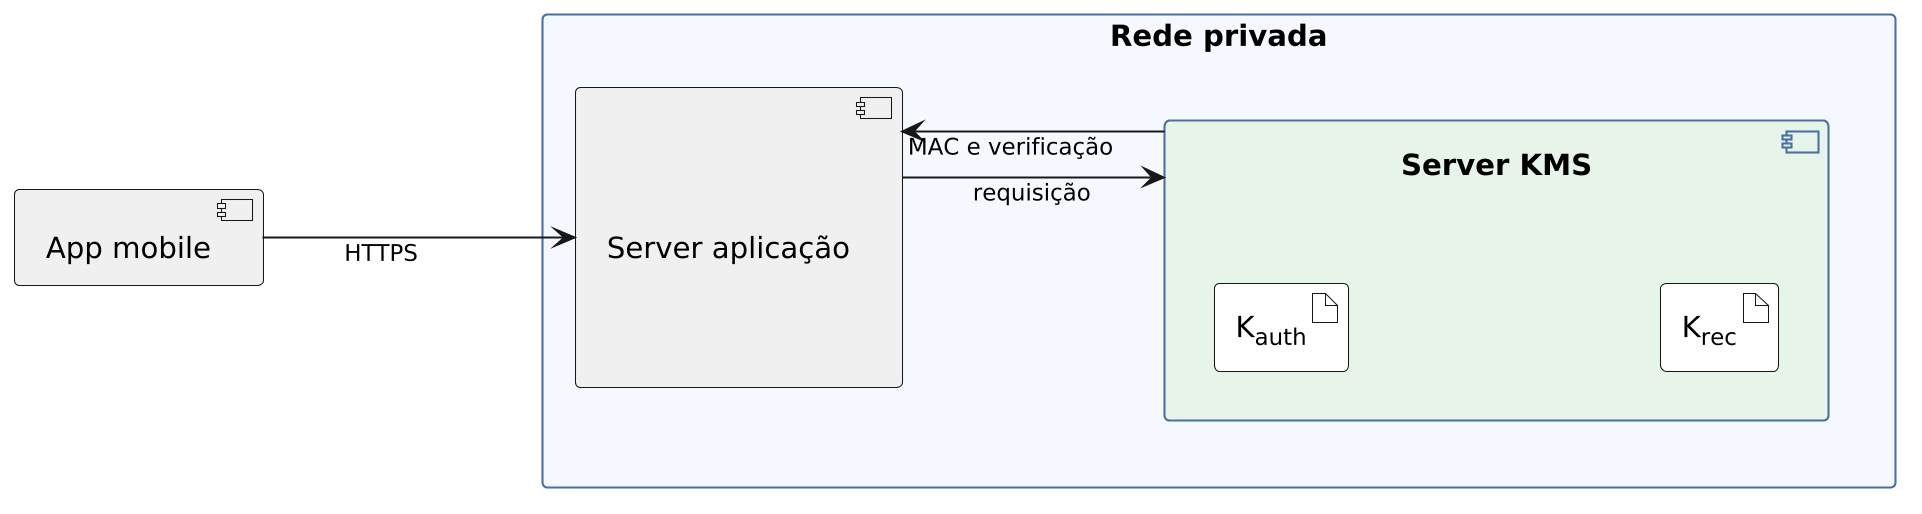
\includegraphics[width=\textwidth]{../../assets/aux-docs/kms-servidor-app.png}
	\legend{Fonte: elaborado pelo autor.}
\end{figure}

\subsection{Garantia das propriedades de segurança}

A coleta no dongle ocorre de maneira offline-first, como mencionado em Investigação-3.pdf. Para que não seja possível alterar blocos guardados no sistema de arquivos do dongle,
assim que o buffer em memória enche o bloco é guardado na memória \textit{flash}, é calculada uma tag de autenticação de 32 bytes via HMAC-SHA256 a partir da chave $K_{rec}$, 
que é salva concatenada ao bloco de dados. Desse modo, caso o dado seja alterado enquanto está na memória, a tag se tornará inválida.

Quando um bloco chega no servidor é possível verificar a tag a partir de uma chamada ao KMS para validar a mensagem e, em seguida, salvar o bloco decodificado. Desse modo, é possível garantir 
integridade e autenticidade do bloco no servidor. Esse desenho garante que ataques do tipo A3.3 da seção \ref{secsec:app-malicioso} não consigam alterar blocos antigos antes de enviar
ao servidor e também garante que não seja possível fabricar novos blocos.

Para que seja possível garantir unicidade, quando um bloco cujo MAC seja válido é recebido pelo servidor, é extraída a \textit{seq} do cabeçalho desse bloco. O servidor verifica se um
bloco com o mesmo valor de \textit{seq} foi recebido, descartando o bloco em caso positivo. Assim, garante-se que um atacante não consiga repetir blocos antigos para alterar os registros
no servidor, como foi modelado para o adversário do tipo AD2 no ataque A3.4 da seção \ref{secsec:app-malicioso}. 

Para que seja possível garantir completude detectável, é necessário que o servidor consiga identificar com exatidão qual foi o número \textit{seq} no último bloco recebido, $ACK_{seq}$, a fim
de que seja possível comparar com o \textit{seq} do último bloco medido pelo dongle, o $HEAD_{seq}$, sendo a diferença $HEAD_{seq} - ACK_{seq}$ entre esses valores a quantidade de blocos
que estão com envio pendente para o server; ao mesmo tempo, todos os blocos com $seq \leq ACK_{seq}$ já foram recebidos e processados, podendo ser excluídos da \textit{flash}. Para garantir sequência e ordem, 
o servidor apenas aceita pacotes cujo valor de seq é exatamente $ACK_{seq} + 1$, descartando pacotes fora de 
ordem (Go-Back-N). Essa dinâmica é ilustrada na \autoref{fig:fila-ack-head}.

Assim, com essa modelagem, é possível garantir ordem e completude detectável, impedindo que as medidas sejam reordenadas ou que sejam criadas lacunas entre diferentes medidas.

\begin{figure}[H]
	\centering
	\caption{Fila de blocos no dongle e a posição de $ACK_{seq}$ e $HEAD_{seq}$}
	\label{fig:fila-ack-head}
	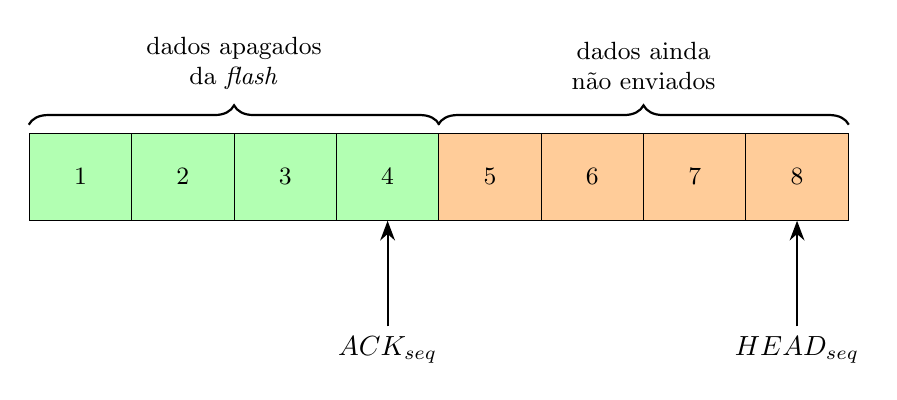
\begin{tikzpicture}[
		bloco/.style={draw, minimum width=1.3cm, minimum height=1.1cm, inner sep=0pt, font=\small},
		enviado/.style={bloco, fill=green!30},
		pendente/.style={bloco, fill=orange!40},
		ponteiro/.style={-{Stealth[length=2.5mm]}, thick},
		chave/.style={decorate, decoration={brace, amplitude=7pt}, thick},
		rotulo/.style={align=center, font=\small}
	]
		% Blocos 1..8, do mais antigo ao mais recente
		\foreach \i in {1,...,4} {
			\node[enviado] (b\i) at (1.3*\i, 0) {\i};
		}
		\foreach \i in {5,...,8} {
			\node[pendente] (b\i) at (1.3*\i, 0) {\i};
		}

		% Ponteiros por baixo dos blocos
		\draw[ponteiro] (b4.south |- 0,-1.9) -- (b4.south);
		\node[anchor=north] at (b4.south |- 0,-1.9) {$ACK_{seq}$};
		\draw[ponteiro] (b8.south |- 0,-1.9) -- (b8.south);
		\node[anchor=north] at (b8.south |- 0,-1.9) {$HEAD_{seq}$};

		% Chaves por cima dos blocos
		\draw[chave] ([yshift=3pt]b1.north west) -- ([yshift=3pt]b4.north east)
			node[rotulo, midway, above=9pt] {dados apagados\\da \textit{flash}};
		\draw[chave] ([yshift=3pt]b5.north west) -- ([yshift=3pt]b8.north east)
			node[rotulo, midway, above=9pt] {dados ainda\\não enviados};
	\end{tikzpicture}
	\legend{Fonte: elaborado pelo autor.}
\end{figure}

Uma limitação real desse modelo vem da dependência do app para conexão com a internet. Um app malicioso pode deliberadamente parar de encaminhar comunicações entre o dongle e o server, ocasionando
a omissão de medidas e inviabilização da conexão via handshake, como está modelado nos ataques A3.2 e A3.7 da seção \ref{secsec:app-malicioso}. Mesmo que não seja possível mitigar diretamente esse
tipo de ataque, a falta dos dados é detectável do lado do servidor, podendo gerar um alerta.

\subsection{Riscos de sincronização} \label{subsec:riscos-sincronizacao}

O fato de o servidor apenas aceitar valores de $seq$ exatamente iguais a $ACK_{seq} + 1$ pode gerar problema de sincronização em três casos diferentes: quando ocorre perda de energia, o valor de $seq$
é perdido, pois ele é armazenado apenas em RAM, uma vez que seu valor muda muito e desgastaria bastante a NVS reescrevê-lo a todo bloco gerado; quando um bloco salvo na \textit{flash} é corrompido,
a verificação de HMAC falha no servidor e ele é rejeitado e, como não há bloco válido com aquele número de $seq$, o servidor não consegue mais receber blocos; e, por fim, quando a \textit{flash} enche
antes de os blocos serem confirmados, o dongle descarta os blocos mais antigos (Investigação-3, seção 2.4.6), de modo que os blocos a partir de $ACK_{seq} + 1$ podem deixar de existir. Para abordar
esses problemas, são usados dois blocos marcadores, BOOT e LOSS, para os dois primeiros casos, e o campo $TAIL_{seq}$ do \textit{handshake} para o terceiro.

Os marcadores BOOT e LOSS não são novos tipos de mensagem: são blocos com o mesmo formato dos blocos de dados, cujo conteúdo é um único registro marcador no lugar das leituras de PID, e por isso
ocupam um $seq$ e percorrem o mesmo fluxo dos blocos de dados até o servidor. O app não os distingue de um bloco comum. Como o marcador faz parte do conteúdo autenticado pela tag, o app não consegue
forjar um LOSS nem transformar um bloco de dados em marcador; o formato exato dos registros marcadores é detalhado na seção \ref{sec:app-ble-dongle}.

Para o bloco de BOOT, é necessário manter uma reserva de $seq$ na NVS para que o contador retome a partir do valor da reserva sempre que perder alimentação. Uma sugestão para esse valor é sempre
armazenar o valor de $seq + 64$ na NVS a cada $64$ blocos gerados e gravados na \textit{flash}. Sempre que o dongle perder energia, ao ser religado ele deve ler o valor da reserva $seq$ da NVS, retomar a contagem a partir dele e,
por fim, gravar na \textit{flash} um novo bloco com $seq$ igual à reserva $R$, cujo único registro é o marcador BOOT com $[from\_seq, to\_seq] = [$último $seq$ na \textit{flash} $+ 1$, $R - 1]$. O
cabeçalho desse bloco já leva o novo $boot\_id$. O servidor aceita esse bloco, mesmo com $seq > ACK_{seq} + 1$, se $from\_seq = ACK_{seq} + 1$ e $to\_seq = seq - 1$; nesse caso, registra a faixa como
lacuna com causa BOOT e faz $ACK_{seq} = seq$.

\begin{figure}[H]
	\centering
	\caption{Reserva de $seq$ na NVS e geração do bloco de BOOT após perda de energia}
	\label{fig:reserva-seq-boot}
	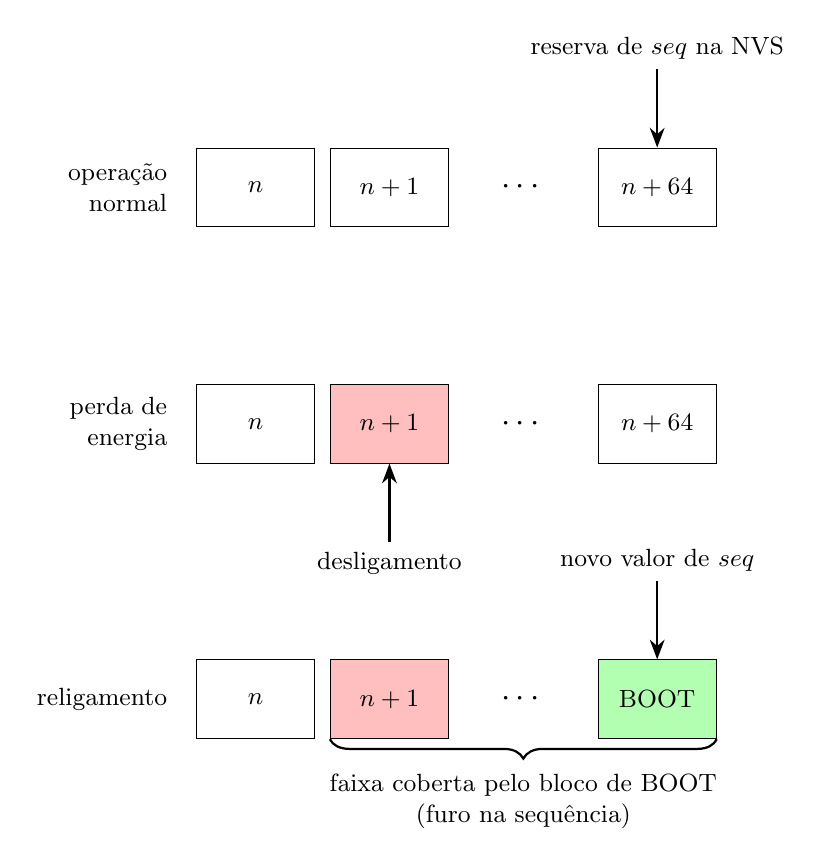
\begin{tikzpicture}[
		bloco/.style={draw, minimum width=1.5cm, minimum height=1cm, inner sep=0pt, font=\small},
		boot/.style={bloco, fill=green!30},
		queda/.style={bloco, fill=red!25},
		reticencias/.style={minimum width=1.5cm, font=\large},
		ponteiro/.style={-{Stealth[length=2.5mm]}, thick},
		chave/.style={decorate, decoration={brace, amplitude=7pt, mirror}, thick},
		rotulo/.style={align=center, font=\small},
		linha/.style={anchor=east, align=right, font=\small}
	]
		% Linha 1: operação normal e reserva de seq na NVS
		\node[bloco] (a0) at (0,0) {$n$};
		\node[bloco] (a1) at (1.7,0) {$n+1$};
		\node[reticencias] (a2) at (3.4,0) {$\cdots$};
		\node[bloco] (a3) at (5.1,0) {$n+64$};
		\node[linha] at (-1,0) {operação\\normal};
		\draw[ponteiro] ([yshift=1cm]a3.north) -- (a3.north);
		\node[rotulo, above] at ([yshift=1cm]a3.north) {reserva de $seq$ na NVS};

		% Linha 2: desligamento no meio da fila
		\node[bloco] (b0) at (0,-3) {$n$};
		\node[queda] (b1) at (1.7,-3) {$n+1$};
		\node[reticencias] (b2) at (3.4,-3) {$\cdots$};
		\node[bloco] (b3) at (5.1,-3) {$n+64$};
		\node[linha] at (-1,-3) {perda de\\energia};
		\draw[ponteiro] ([yshift=-1cm]b1.south) -- (b1.south);
		\node[rotulo, below] at ([yshift=-1cm]b1.south) {desligamento};

		% Linha 3: religamento e bloco de BOOT
		\node[bloco] (c0) at (0,-6.5) {$n$};
		\node[queda] (c1) at (1.7,-6.5) {$n+1$};
		\node[reticencias] (c2) at (3.4,-6.5) {$\cdots$};
		\node[boot] (c3) at (5.1,-6.5) {BOOT};
		\node[linha] at (-1,-6.5) {religamento};
		\draw[ponteiro] ([yshift=1cm]c3.north) -- (c3.north);
		\node[rotulo, above] at ([yshift=1cm]c3.north) {novo valor de $seq$};
		\draw[chave] (c1.south west) -- (c3.south east)
			node[rotulo, midway, below=9pt] {faixa coberta pelo bloco de BOOT\\(furo na sequência)};
	\end{tikzpicture}
	\legend{Fonte: elaborado pelo autor.}
\end{figure}

Para o caso de corrompimento, é necessário verificar se houve corrompimento no bloco sempre antes de enviá-lo ao app para ir ao servidor e, caso seja detectado, o dongle gera, no momento do envio,
um novo bloco com $seq$ igual ao do primeiro bloco corrompido, cujo único registro é o marcador LOSS com a faixa $[from\_seq, to\_seq]$ afetada. Como o cabeçalho original pode estar corrompido,
$boot\_id$ e $t_{ms}$ vão zerados. Esse bloco não é gravado na \textit{flash}: em um reenvio, ele é regenerado. O servidor o aceita se $seq = from\_seq = ACK_{seq} + 1$, registra a faixa como lacuna
com causa LOSS e faz $ACK_{seq} = to\_seq$; o dongle avança o cursor para $to\_seq + 1$. Seria possível verificar a integridade do bloco apenas calculando o hash, mas isso é computacionalmente custoso
para recalcular em todo bloco. Por isso, é mais eficiente salvar um CRC32, calculado sobre os dados e a tag HMAC, em todo bloco e verificar esse CRC32 antes de mandar para o app. O uso do CRC32 adiciona apenas 4 bytes por
bloco, que é justificável depois das otimizações feitas anteriormente.

Para o caso de \textit{flash} cheia, um bloco marcador não serve, pois os blocos descartados já não existem para serem substituídos. O dongle informa então, na resposta do \textit{handshake} (seção
\ref{subsec:handshake}), o $TAIL_{seq}$. Se $ACK_{seq} + 1 < TAIL_{seq} \leq HEAD_{seq} + 1$, o servidor registra a faixa $[ACK_{seq} + 1, TAIL_{seq} - 1]$ como lacuna com causa OVERFLOW e avança
$ACK_{seq}$ para $TAIL_{seq} - 1$, valor devolvido ao dongle na confirmação do mesmo \textit{handshake}. Se $TAIL_{seq} > HEAD_{seq} + 1$, a resposta é inconsistente e é rejeitada. Se o descarte
ocorrer no meio de uma sessão, atingindo blocos acima do ACK local, o dongle invalida a sessão e sinaliza ao app que um novo \textit{handshake} é necessário (seção \ref{sec:app-ble-dongle}), trazendo
o $TAIL_{seq}$ atualizado.

O $TAIL_{seq}$ é autenticado com $K_{auth}$ e amarrado ao \textit{nonce} $N_S$, então o app não consegue forjar uma perda. Ele ainda pode provocá-la, deixando de pedir lotes (A3.2), mas a perda chega
ao servidor declarada, com faixa e causa.

\subsection{Especificação do processo de handshake} \label{subsec:handshake}

Quando o dongle começa sua operação principal, ele salva um $boot_id$ na NVS que serve até ele deixar de ser alimentado ou até entrar e sair de deep sleep.
Enquanto o dongle estiver offline, a coleta dos PIDs de telemetria vai continuar ocorrendo como esperado, com blocos passando pelo buffer em RAM e indo
para a memória \textit{flash} com suas tags de autenticação e um CRC32.

Assim que há um pedido de handshake do dongle ou assim que o app se conecta com a internet, o \textit{handshake}, utilizando os parâmetros definidos na tabela \ref{table:params-handshake},
começa e segue a seguinte sequência de passos, abstraindo a intermediação do app:

\begin{enumerate}
	\item Dongle pede que $S_{App}$ envie um desafio
	\item Server anota $S1$
	\item Server envia um bloco desafio tipo 0x01 para o dongle contendo: $c_S$, $N_S$, $ACK_{seq}$, $c_{conf}$, $flags_c$, $diag_min$ e $tag$ (47 bytes) com destino ao dongle
	\item Dongle responde um bloco tipo 0x02 contendo: $c_S$, $N_S$, $TAIL_{seq}$, $HEAD_{seq}$, $boot\_id$, $t_{ms}$ e $tag$ (50 bytes) com destino ao server
	\item Com $S2$, o server fecha a âncora de tempo para $boot\_id$ segundo algoritmo de Cristian e, com $TAIL_{seq}$, verifica se houve descarte por \textit{flash} cheia, atualizando $ACK_{seq}$
	(seção \ref{subsec:riscos-sincronizacao})
	\item Server envia bloco ACK tipo 0x04 contendo: $ACK_{seq}$, $c_{conf}$, $flags_a$, e $tag$ (25 bytes) com destino ao dongle
	\item Server envia, com destino ao app, um token JWT válido para receber blocos do app.
\end{enumerate}

\begin{figure}[H]
	\centering
	\caption{Diagrama de sequência do \textit{handshake} e da âncora de tempo}
	\label{fig:sequencia-handshake}
	% Fonte PlantUML: ../assets/aux-docs/plantuml/handshake-sequencia.puml
	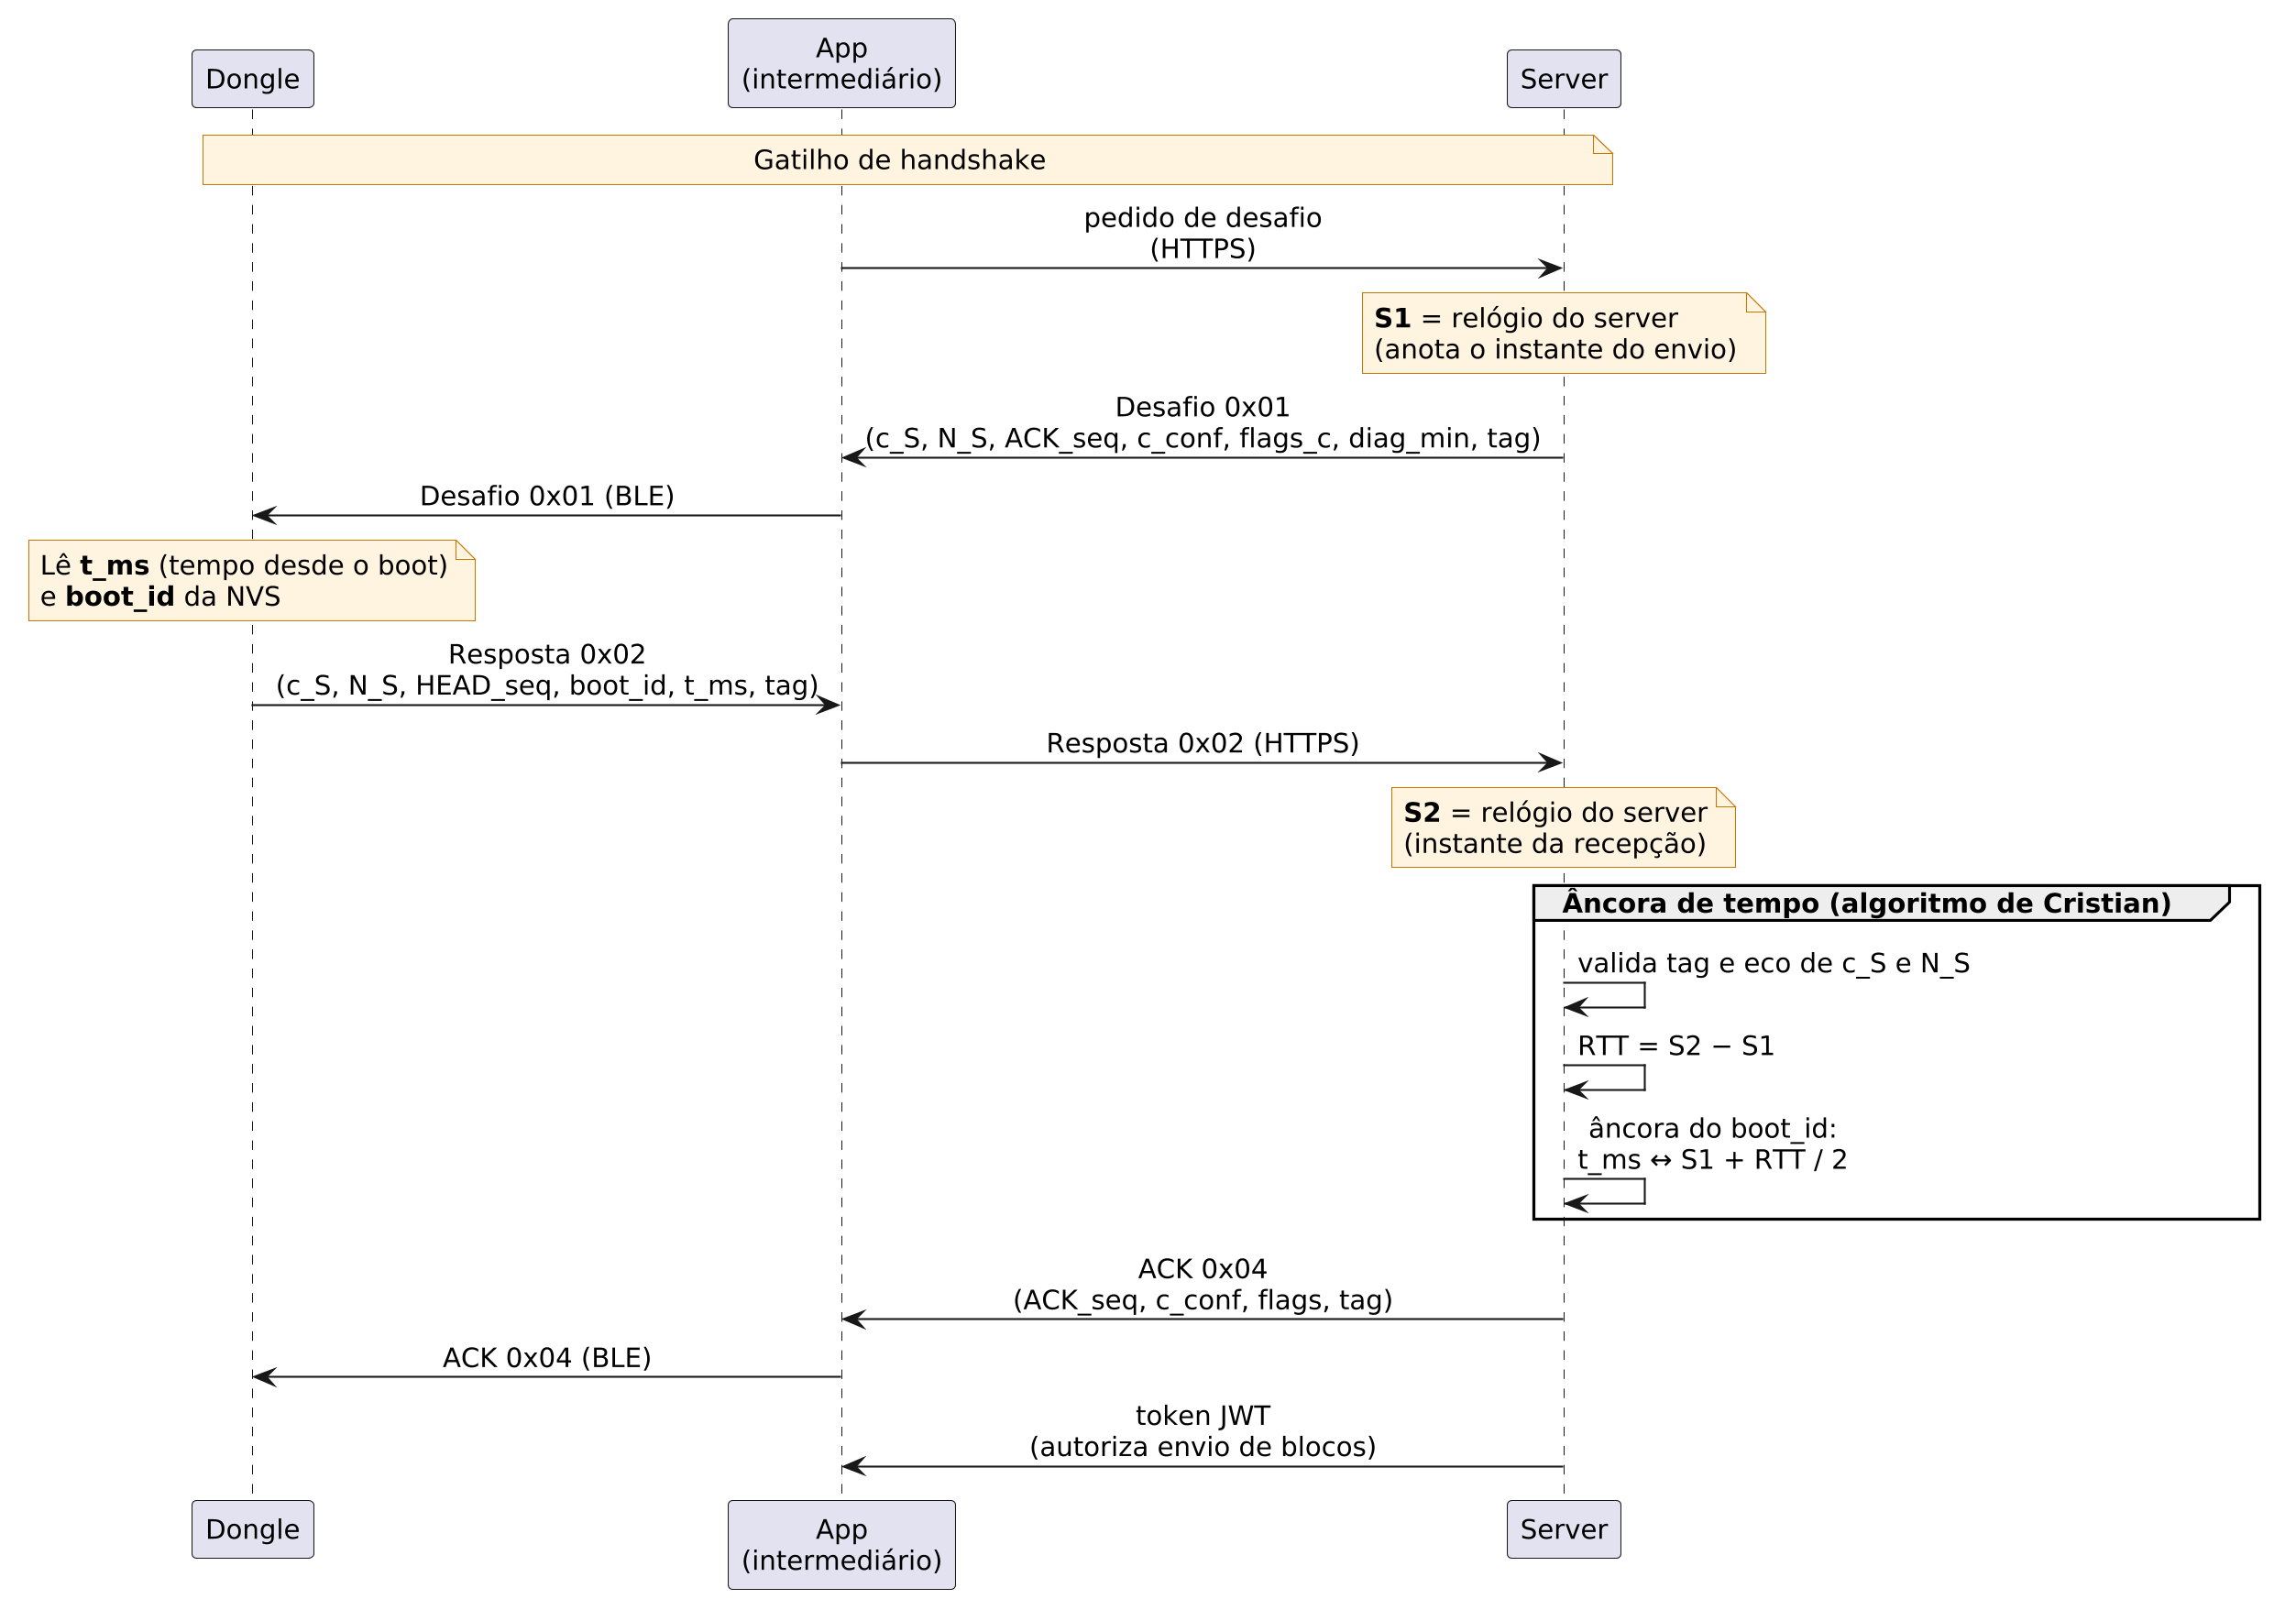
\includegraphics[width=\textwidth]{../../assets/aux-docs/handshake-sequencia.png}
	\legend{Fonte: elaborado pelo autor.}
\end{figure}

\begin{table}[H]
	\centering
	\caption{Parâmetros do processo de \textit{handshake}}
	\label{table:params-handshake}
	\begin{tabular}{|>{\centering\arraybackslash}m{0.15\textwidth}|>{\raggedright\arraybackslash}m{0.45\textwidth}|>{\centering\arraybackslash}m{0.15\textwidth}|>{\centering\arraybackslash}m{0.1\textwidth}|}
		\hline
		\textbf{Parâmetro} & \textbf{Descrição} & \textbf{Origem} & \textbf{Bytes} \\
		\hline
		$c_{S}$ & Contador de desafios associado ao dongle pelo seu \textit{DevId} & $S_{App}$ & 4 \\
		\hline
		$N_{S}$ & \textit{Nonce} que identifica o desafio & $S_{App}$ & 16 \\
		\hline
		$ACK_{seq}$ & Fronteira que indica o último \textit{seq} recebido pelo server & $S_{App}$ & 4 \\
		\hline
		$c_{conf}$ & $c_{S}$ do último desafio aceito para conferência & $S_{App}$ & 4 \\
		\hline
		$flags_c$ & Bit 0: indica se ativa modo diagnóstico; Outros bits reservados & $S_{App}$ & 1 \\
		\hline
		$diag_min$ & Tempo em minutos que o dispositivo ficará em modo diagnóstico & $S_{App}$ & 2 \\
		\hline
		$TAIL_{seq}$ & Valor de $seq$ do bloco mais antigo ainda na \textit{flash}; $HEAD_{seq} + 1$ se a \textit{flash} está vazia & Dongle & 4 \\
		\hline
		$HEAD_seq$ & Valor de $seq$ do último bloco gravado no LittleFS & Dongle & 4 \\
		\hline
		$boot\_id$ & O valor de ID do \textit{boot} atual do dongle & Dongle & 2 \\
		\hline
		$t_{ms}$ & Tempo em milissegundos desde o boot no instante da resposta & Dongle & 4 \\
		\hline
		$flags_a$ & Bit 0: indica falha na sincronização de tempo, \textit{handshake} deve ser repetido; Outros bits reservados & $S_{App}$ & 1 \\
		\hline
		$tag$ & Tag calculada via HMAC-SHA256 & Dongle ou $S_{App}$ & 16 \\
		\hline
	\end{tabular}
\end{table}

Para emitir o desafio, o server incrementa $c_S$, sorteia $N_s$ e guarda o novo desafio no banco de dados associando ao $DevId$ que o pediu.
Ao receber o desafio, o dongle confere a tag e verifica que $c_S$ é maior do que o último aceito, valor que está salvo na NVS, garantindo que
não está respondendo um desafio repetido; caso $ACK_{local} < ACK_{seq} \leq HEAD_{seq}$, em que $ACK_{local}$ é o último valor de ACK conhecido pelo dongle, os blocos até $ACK_{seq}$ são removidos da 
\textit{flash}. Na resposta do dongle, o $N_S$ ecoado serve para garantir que a resposta enviada é de um novo desafio. Ao avaliar a resposta, o 
server confere, além da tag, se o eco de $c_S$ e de $N_S$ corresponde ao desafio guardado no banco de dados, se ele ainda não foi usado e se não expirou; caso positivo, aplica a regra do $TAIL_{seq}$
(seção \ref{subsec:riscos-sincronizacao}) e envia o bloco $ACK$, com o $ACK_{seq}$ resultante e \textit{flags} zeradas, e o token JWT.

Para o cálculo da tag das mensagens de handshake, que são relacionadas à autenticação, é usada a chave $K_{auth}$ para gerar o HMAC-SHA256 segundo a 
equação \ref{eq:hmac-sha256-auth}, que é truncado em seguida para 16 bytes a fim de economizar banda na transmissão. Aqui é possível truncar devido ao 
ato de o server ter permissão de gerar MACs com $K_{auth}$ no KMS, o que possibilita o servidor gerar o HMAC e comparar os primeiros 16 bytes; como o server 
não consegue gerar HMAC para $K_{rec}$, não é possível truncar o HMAC dos blocos, mostrado na equação \ref{eq:hmac-sha256-rec}, sem perder o isolamento de 
responsabilidades no KMS.

No cálculo do HMAC em \ref{eq:hmac-sha256-auth}, além da chave e do payload, são adicionados no cálculo da tag alguns separadores de contexto para evitar
que uma tag válida seja reaproveitada em outro contexto para um payload de mesmo valor. O termo "MALCONG" é um rótulo fixo para esse projeto, 
o \textit{tipo} representa o tipo de bloco que está sendo calculado no MAC. A figura \ref{fig:blocos-handshake} mostra os tipos de blocos utilizados no handshake.
Já a equação \ref{eq:hmac-sha256-rec} mostra o cálculo do HMAC feito para os blocos guardados na \textit{flash}, também usando o rótulo fixo "MALCONG" e o \textit{DevId},
completando com a constante $0x03$ para manter a convenção de adicionar o tipo de mensagem no cálculo do HMAC; é importante lembrar que o bloco engloba seu próprio cabeçalho,
que contém o $seq$, não sendo necessário adicioná-lo novamente.

O diagrama de sequência da figura \ref{fig:sequencia-handshake} mostra o fluxo de comunicação, considerando a intermediação do app. O gatilho de handshake ocorre nas seguintes
situações: boot do dongle ou nova conexão BLE, eventos que zeram a flag na RAM do dongle que indica se houve handshake, fazendo com que o dongle peça um handshake para o app
a partir das mensagens que serão especificadas em \ref{sec:app-ble-dongle}; token JWT perto de expirar, o que força um novo handshake para nova emissão de token JWT; ou âncora rejeitada,
que força um novo handshake para sincronização.

Sobre a âncora de tempo, uma limitação conhecida é quando um boot fica todo seu ciclo de vida em uma conexão, o que faz com que o boot fique sem sincronização de relógio completa.


\begin{equation} \label{eq:hmac-sha256-auth}
	tag = \text{HMAC-SHA256}_{K_{auth}}("MALCONG"\ ||\ \text{tipo}\ ||\ DevId\ ||\ \text{payload})
\end{equation}

\begin{equation} \label{eq:hmac-sha256-rec}
	tag = \text{HMAC-SHA256}_{K_{rec}}("MALCONG"\ ||\ \text{0x03} ||\ DevId\ ||\ \text{bloco})
\end{equation}


\begin{figure}[H]
	\centering
	\caption{Blocos utilizados no \textit{handshake}}
	\label{fig:blocos-handshake}
	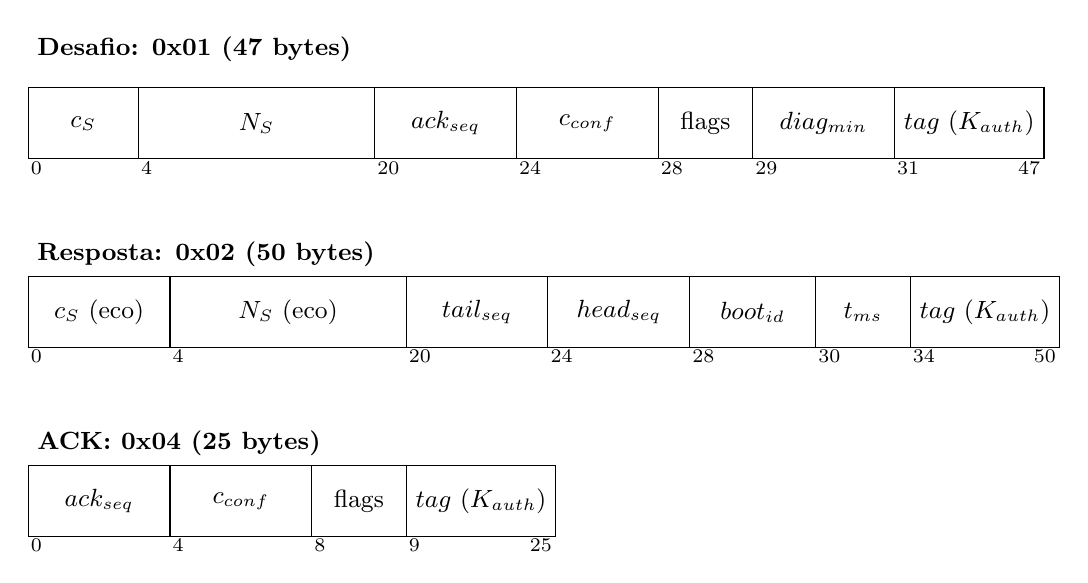
\begin{tikzpicture}[
		campo/.style={draw, minimum height=0.9cm, inner sep=1pt, font=\small, align=center},
		posini/.style={font=\scriptsize, anchor=north west, inner sep=1pt},
		posfim/.style={font=\scriptsize, anchor=north east, inner sep=1pt},
		titulo/.style={font=\small\bfseries, anchor=south west}
	]
		% \campo{x}{y}{largura}{texto}{posição inicial}
		\newcommand{\campo}[5]{%
			\node[campo, anchor=north west, minimum width=#3 cm] at (#1,#2) {#4};
			\node[posini] at (#1,#2-0.9) {#5};}
		% \fim{x}{y}{posição final}
		\newcommand{\fim}[3]{\node[posfim] at (#1,#2-0.9) {#3};}

		% Desafio (tipo 0x01, servidor -> dongle)
		\node[titulo] at (0,0.2) {Desafio: 0x01 (47 bytes)};
		\campo{0}{0}{1.4}{$c_S$}{0}
		\campo{1.4}{0}{3.0}{$N_S$}{4}
		\campo{4.4}{0}{1.8}{$ack_{seq}$}{20}
		\campo{6.2}{0}{1.8}{$c_{conf}$}{24}
		\campo{8.0}{0}{1.2}{flags}{28}
		\campo{9.2}{0}{1.8}{$diag_{min}$}{29}
		\campo{11.0}{0}{1.9}{$tag$ ($K_{auth}$)}{31}
		\fim{12.9}{0}{47}

		% Resposta (tipo 0x02, dongle -> servidor)
		\node[titulo] at (0,-2.4) {Resposta: 0x02 (50 bytes)};
		\campo{0}{-2.4}{1.8}{$c_S$ (eco)}{0}
		\campo{1.8}{-2.4}{3.0}{$N_S$ (eco)}{4}
		\campo{4.8}{-2.4}{1.8}{$tail_{seq}$}{20}
		\campo{6.6}{-2.4}{1.8}{$head_{seq}$}{24}
		\campo{8.4}{-2.4}{1.6}{$boot_{id}$}{28}
		\campo{10.0}{-2.4}{1.2}{$t_{ms}$}{30}
		\campo{11.2}{-2.4}{1.9}{$tag$ ($K_{auth}$)}{34}
		\fim{13.1}{-2.4}{50}

		% ACK (tipo 0x04, servidor -> dongle)
		\node[titulo] at (0,-4.8) {ACK: 0x04 (25 bytes)};
		\campo{0}{-4.8}{1.8}{$ack_{seq}$}{0}
		\campo{1.8}{-4.8}{1.8}{$c_{conf}$}{4}
		\campo{3.6}{-4.8}{1.2}{flags}{8}
		\campo{4.8}{-4.8}{1.9}{$tag$ ($K_{auth}$)}{9}
		\fim{6.7}{-4.8}{25}
	\end{tikzpicture}
	\legend{Fonte: elaborado pelo autor.}
\end{figure}

\section{Integração entre BLE e HTTPS/TLS para troca de dados entre dongle e servidor}

O app se comunica com o dongle por meio de BLE. Como já foi modelado na seção \ref{secsec:comunicacao-wireless}, o BLE
é um enlace sem autenticidade, confidencialidade e integridade caso não seja usado o padrão LESC, o que abre
a possibilidade de ataques do tipo A1.2, A1.3 e A1.4 da seção \ref{secsec:comunicacao-wireless}. Por isso, o celular se comunicará
apenas depois de um pareamento seguindo o padrão LESC, ajustando o firmware do dongle para aceitar apenas conexões LESC.

O método de pareamento dentre os definidos na tabela \ref{lesc:metodos} será o Just Works, devido ao fato de o dongle não
ter nenhuma capacidade de Input/Output. Isso expõe a conexão ao ataque A1.3, de \textit{Man in The Middle}, modelado na seção
\ref{secsec:comunicacao-wireless} para um adversário do tipo AD1, que está perto do carro no momento da conexão. 

No entanto, são tomadas algumas medidas para diminuir esse risco:
o dongle aceita pareamentos apenas em um intervalo de tempo definido depois de apertar um botão físico no dongle, o que deixa menos
margem para o atacante conseguir interceptar a conexão; além disso, é permitido apenas um bond (pareamento) por vez, sendo que apertar o 
botão derruba todos os pareamentos feitos, o que desconecta um atacante. Essas medidas também evitam ataque do tipo DoS, modelados 
na seção \ref{secsec:comunicacao-wireless} como A1.5

\subsection{Serviços e blocos BLE para comunicação entre app e dongle} \label{sec:app-ble-dongle}

Os comandos ELM327, incluindo os comandos customizados de configuração definidos no projeto, são enviados do app para o dongle a partir 
do serviço NUS. Enquanto isso, os comandos de handshake e envio de blocos passam por um outro serviço criado para o projeto, chamado 
SYNC. Assim como o NUS, o SYNC expõe uma característica RX, na qual o dongle recebe dados do app, e uma característica TX, na qual 
o dongle envia dados para o app; no entanto, enquanto o NUS recebe texto, o serviço SYNC envia e recebe dados binários. Com essa separação,
cada fluxo de dados entre app e dongle fica separado e com suas próprias responsabilidades, ajudando na remontagem de blocos a partir dos fragmentos.

Além dos tipos de blocos definidos no handshake, existem mais alguns tipos que precisam ser usados para orquestrar a comunicação entre app e dongle, sendo
todos eles apresentados na tabela \ref{table:tipos-blocos}. Quando são enviados via BLE no SYNC\_RX, como convenção do projeto, os blocos são estruturados no formato TLV (type, length, value), 
sendo 3 bytes concatenados no início de cada bloco, o primeiro byre representa o tipo e os outros dois o comprimento do corpo da mensagem, ou seja, sem contar o tipo e comprimento. Além disso, quando são
enviados no SYNC\_TX, também é necessário englobar o bloco TLV em um enquadramento com um byte de controle na frente: nesse byte de controle, o bit 7 vale 1 quando for um início de mensagem e os bits de 6 a 0
servem de contador de modo que o primeiro fragmento da mensagem completa começa em 0 e a cada fragmento vai somando 1 até 127, voltando para 0 no próximo fragmento, o que permite detectar fragmentos faltantes.
Para remontar, então, basta desencapsular e juntar os fragmentos na ordem correta até o comprimento marcado ser alcançado.
Isso é necessário pelo fato de as mensagens do SYNC\_TX poderem ser fragmentadas em vários pacotes BLE. O formato do pacote de cada característica do SYNC pode ser visto na figura \ref{fig:sync-tvl}.

\begin{figure}[H]
	\centering
	\caption{Formato dos dados nas características RX e TX do serviço SYNC}
	\label{fig:sync-tvl}
	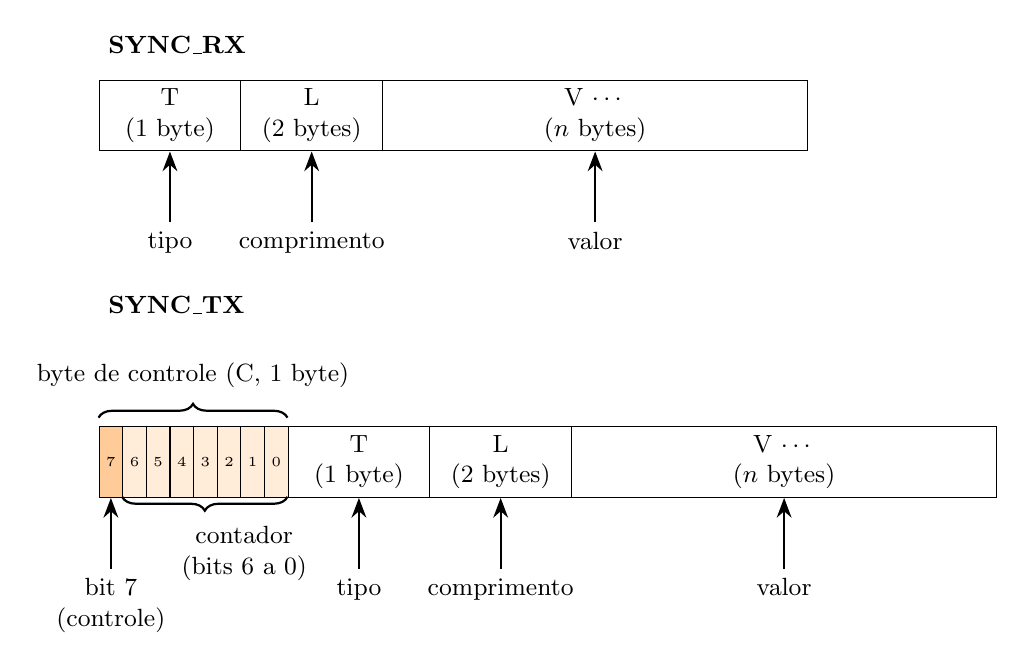
\begin{tikzpicture}[
		campo/.style={draw, minimum height=0.9cm, inner sep=1pt, font=\small, align=center},
		controle/.style={campo, fill=orange!40},
		ponteiro/.style={-{Stealth[length=2.5mm]}, thick},
		rotulo/.style={align=center, font=\small, anchor=north},
		chave/.style={decorate, decoration={brace, amplitude=5pt}, thick},
		titulo/.style={font=\small\bfseries, anchor=south west}
	]
		% \campo{x}{y}{largura}{texto}{estilo}{id}
		\newcommand{\campo}[6]{\node[#5, anchor=north west, minimum width=#3 cm] (#6) at (#1,#2) {#4};}
		% \seta{id}{texto}
		\newcommand{\seta}[2]{\draw[ponteiro] ([yshift=-0.9cm]#1.south) -- (#1.south);
			\node[rotulo] at ([yshift=-0.9cm]#1.south) {#2};}

		% SYNC_RX: formato TLV
		\node[titulo] at (0,0.2) {SYNC\_RX};
		\campo{0}{0}{1.8}{T\\(1 byte)}{campo}{rt}
		\campo{1.8}{0}{1.8}{L\\(2 bytes)}{campo}{rl}
		\campo{3.6}{0}{5.4}{V $\cdots$\\($n$ bytes)}{campo}{rv}
		\seta{rt}{tipo}
		\seta{rl}{comprimento}
		\seta{rv}{valor}

		% SYNC_TX: TLV precedido por um byte de controle
		\node[titulo] at (0,-3.1) {SYNC\_TX};
		% byte de controle: 8 bits, apenas o primeiro (bit de controle) é destacado
		\campo{0}{-4.4}{0.3}{\tiny 7}{controle}{tc}
		\foreach \i/\b in {1/6,2/5,3/4,4/3,5/2,6/1,7/0} {
			\node[campo, fill=orange!15, anchor=north west, minimum width=0.3cm, font=\tiny] at (0.3*\i,-4.4) {\b};
		}
		\node[coordinate] (contini) at (0.3,-5.3) {};
			\node[coordinate] (contfim) at (2.4,-5.3) {};
			\draw[chave, decoration={brace, mirror, amplitude=5pt}] (contini) -- (contfim)
				node[rotulo, midway, anchor=north, yshift=-7pt, xshift=0.5cm] {contador\\(bits 6 a 0)};
			\node[coordinate] (cini) at (0,-4.4) {};
		\node[coordinate] (cfim) at (2.4,-4.4) {};
		\draw[chave] ([yshift=3pt]cini) -- ([yshift=3pt]cfim)
			node[rotulo, midway, anchor=south, yshift=7pt] {byte de controle (C, 1 byte)};
		\campo{2.4}{-4.4}{1.8}{T\\(1 byte)}{campo}{tt}
		\campo{4.2}{-4.4}{1.8}{L\\(2 bytes)}{campo}{tl}
		\campo{6.0}{-4.4}{5.4}{V $\cdots$\\($n$ bytes)}{campo}{tv}
		\seta{tc}{bit 7\\(controle)}
		\seta{tt}{tipo}
		\seta{tl}{comprimento}
		\seta{tv}{valor}
	\end{tikzpicture}
	\legend{Fonte: elaborado pelo autor.}
\end{figure}



\begin{table}[H]
	\centering
	\caption{Tipos de blocos trocados entre servidor, app e dongle}
	\label{table:tipos-blocos}
	\begin{tabular}{|>{\centering\arraybackslash}m{0.08\textwidth}|>{\raggedright\arraybackslash}m{0.17\textwidth}|>{\centering\arraybackslash}m{0.15\textwidth}|>{\raggedright\arraybackslash}m{0.42\textwidth}|}
		\hline
		\textbf{Tipo} & \textbf{Nome} & \textbf{Tamanho (bytes)} & \textbf{Parâmetros (bytes)} \\
		\hline
		0x01 & Desafio & 45 ou 47 & $c_{S}$ (4), $N_{S}$ (16), $ACK_{seq}$ (4), $c_{conf}$ (4), $flags$ (1), $diag\_min$ (2, só com o bit 0 das $flags$), $tag$ (16) \\
		\hline
		0x02 & Resposta & 50 & $c_{S}$ (4, eco), $N_{S}$ (16, eco), $TAIL_{seq}$ (4), $HEAD_{seq}$ (4), $boot\_id$ (2), $t_{ms}$ (4), $tag$ (16) \\
		\hline
		0x03 & Bloco & 55 a 1.056 & $seq$ (4), $boot\_id$ (2), $t_{ms}$ inicial (4), tamanho (2), registros (até 1.012), $tag$ (32); inclui os blocos marcadores BOOT e LOSS (seção \ref{subsec:riscos-sincronizacao}) \\
		\hline
		0x04 & ACK & 25 & $ACK_{seq}$ (4), $c_{conf}$ (4), $flags$ (1), $tag$ (16) \\
		\hline
		0x05 & Pedido de lote & 2 & $K$ (2): blocos ainda não lidos pelo app, limitados pelo espaço livre no \textit{buffer} \\
		\hline
		0x06 & Erro & 1 & código (1) \\
		\hline
		0x07 & Aviso de novo bloco & 13 & $HEAD_{seq}$ (4), $flags$ (1), $DevID$ (8) \\
		\hline
	\end{tabular}
\end{table}

Os blocos do handshake de Desafio (0x01) e ACK (0x04), ao chegarem do servidor no app, são repassados diretamente para SYNC\_RX no formato binário ou, caso necessário, são antes decodificados
a partir da string base64. Enquanto isso, os blocos de Resposta (0x02) e de Envio de Blocos (0x03) são construídos no dongle e, quando chegam no app via SYNC\_TX, são diretamente enviados pelo
app para o servidor no seu respectivo endpoint, havendo codificação para string base64 quando necessário.

Os blocos marcadores BOOT e LOSS, usados para declarar lacunas na sequência (seção \ref{subsec:riscos-sincronizacao}), são blocos 0x03 e são tratados pelo app exatamente como blocos de dados: o app
não os distingue de um bloco com leituras de PID. Seguindo a convenção do registro de GPS (tipo 0xFF), são reservados os tipos de registro 0xFE (BOOT) e 0xFD (LOSS), ambos no formato tipo (1) $\mid$
$\Delta t$ (2) $\mid$ $from\_seq$ (4) $\mid$ $to\_seq$ (4), com 11 bytes; com o cabeçalho de 12 bytes, o bloco marcador tem 23 bytes de conteúdo, mais a tag de 32 bytes. Por serem blocos 0x03, os
marcadores ocupam um $seq$, recebem a tag $K_{rec}$ da equação \ref{eq:hmac-sha256-rec} e percorrem o mesmo fluxo dos blocos de dados: são contados no $HEAD_{seq}$, pedidos via Pedido de lote 0x05,
fragmentados no SYNC\_TX, enviados no \texttt{POST /v1/dongles/blocos} e confirmados pelo ACK 0x04. Como o marcador faz parte do conteúdo autenticado, o app não consegue forjar um LOSS nem
transformar um bloco de dados em marcador.

Quando o dongle dá flush em um bloco para a \textit{flash}, ele envia um aviso de novo bloco (0x07) para o app. Quando esse aviso chega, caso o app já tenha disponível um valor de $ACK_{seq}$ válido, 
ele calcula o valor de quantos blocos estão pendentes de envio a partir de $HEAD_{seq} - ACK_{seq}$, sendo o $HEAD_{seq}$ recebido via aviso. As flags desse bloco de aviso podem ser vistas na tabela
\ref{tab:flags-aviso-novo-bloco}. Caso o app ainda não tenha um handshake válido, o dongle solicita para o app que faça um pedido de desafio para o servidor, iniciando o processo de handshake.

\begin{table}[H]
	\centering
	\caption{\textit{Flags} do aviso de novo bloco}
	\label{tab:flags-aviso-novo-bloco}
	\begin{tabular}{|>{\centering\arraybackslash}m{0.07\textwidth}|>{\raggedright\arraybackslash}m{0.15\textwidth}|>{\raggedright\arraybackslash}m{0.19\textwidth}|>{\raggedright\arraybackslash}m{0.19\textwidth}|>{\raggedright\arraybackslash}m{0.19\textwidth}|}
		\hline
		\textbf{Bit} & \textbf{Significado} & \textbf{Quando liga} & \textbf{Quando desliga} & \textbf{O que o app faz} \\
		\hline
		0 & Sem \textit{handshake} nesta conexão & A cada conexão BLE nova (\textit{flag} em RAM, zerada ao conectar) ou quando o dongle descarta blocos não confirmados por \textit{flash} cheia & Quando chega um ACK com $c_{conf}$ igual ao $c_{S}$ que o dongle respondeu & Faz o \textit{handshake} antes de qualquer pedido de lote \\
		\hline
		1 & Sem \textit{handshake} neste \textit{boot} & A cada \textit{boot} & Igual ao bit 0 & Faz o \textit{handshake}, para o \textit{boot} ganhar uma âncora de tempo \\
		\hline
		2 & \textit{Flash} acima de 80\% & Quando a ocupação da \textit{flash} passa de 80\% & Quando cai abaixo disso, depois que ACKs liberam espaço & Prioriza o envio: lê até encher o \textit{buffer} e envia lotes de 32 em seguida, sem esperar $T_{lat}$, e pode avisar o usuário \\
		\hline
		3 a 7 & Reservados & --- & --- & Ignora \\
		\hline
	\end{tabular}
\end{table}

Ao receber um aviso de novo bloco, o app pede ao dongle os blocos que ainda não leu, com um bloco de Pedido de Lote (0x05) em que $K$ é o mínimo entre os blocos ainda não lidos (diferença entre $HEAD_{seq}$ e o
último $seq$ lido) e o espaço livre no \textit{buffer} do app. Os blocos lidos ficam num \textit{buffer} em memória até serem enviados ao servidor e confirmados. O momento do envio é controlado pelo
parâmetro de latência $T_{lat}$, descrito na seção \ref{subsec:ritmo-envio-buffer}, e cada POST leva no máximo 32 blocos.

É importante notar que o MTU do BLE não suporta um bloco inteiro, que fica negociado em torno de 272 bytes. O bloco completo, como mostra a figura \ref{fig:bloco-completo} terá 1059 bytes, sendo 1 byte com o 
tipo, 2 bytes com o comprimento, 1024 bytes de dados e, por fim, 32 bytes de tag. Os bytes do CRC são conferidos antes de o dongle enviar os blocos via BLE, então não aparecem aqui.

A figura \ref{fig:bloco-completo} mostra o bloco já pronto para a transmissão, enquanto o que é diferente do que fica gravado na \textit{flash} , como mostra a figura \ref{fig:bloco-flash}. O bloco salvo não tem o
envelope de tipo e comprimento, que é só uma convenção para o enquadramento no SYNC\_RX e é montado na hora de enviar; em compensação, tem mais 4 bytes de CRC32 no final, calculados sobre os dados e a tag
(seção \ref{subsec:riscos-sincronizacao}), usados para detectar corrompimento antes do envio. Para montar o bloco da figura \ref{fig:bloco-completo} a partir do que está na flash, o dongle então descarta
o CRC já verificado e acrescenta o envelope TLV com tipo 0x03 e o comprimento.

\begin{figure}[H]
	\centering
	\caption{Estrutura do bloco como gravado na \textit{flash}}
	\label{fig:bloco-flash}
	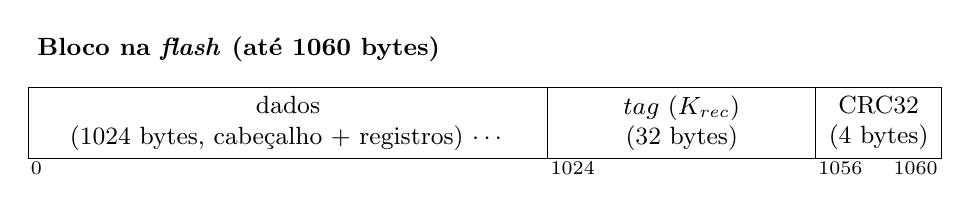
\begin{tikzpicture}[
		campo/.style={draw, minimum height=0.9cm, inner sep=1pt, font=\small, align=center},
		posini/.style={font=\scriptsize, anchor=north west, inner sep=1pt},
		posfim/.style={font=\scriptsize, anchor=north east, inner sep=1pt},
		titulo/.style={font=\small\bfseries, anchor=south west}
	]
		% \campo{x}{y}{largura}{texto}{posição inicial}
		\newcommand{\campo}[5]{%
			\node[campo, anchor=north west, minimum width=#3 cm] at (#1,#2) {#4};
			\node[posini] at (#1,#2-0.9) {#5};}
		% \fim{x}{y}{posição final}
		\newcommand{\fim}[3]{\node[posfim] at (#1,#2-0.9) {#3};}

		\node[titulo] at (0,0.2) {Bloco na \textit{flash} (até 1060 bytes)};
		\campo{0}{0}{6.6}{dados\\(1024 bytes, cabeçalho + registros) $\cdots$}{0}
		\campo{6.6}{0}{3.4}{$tag$ ($K_{rec}$)\\(32 bytes)}{1024}
		\campo{10.0}{0}{1.6}{CRC32\\(4 bytes)}{1056}
		\fim{11.6}{0}{1060}
	\end{tikzpicture}
	\legend{Fonte: elaborado pelo autor.}
\end{figure}

Para enviar os blocos então, o dongle primeiro consolida no formato TLV e, em seguida, divide em fragmentos de até $MTU - 4$ bytes, adicionando o byte de controle, sendo que o bit 7 do byte de controle vale 1 somente
no primeiro fragmento de cada bloco da flash. Esses blocos são então mandados via BLE para o app, que remonta o bloco original da flash. Quando os blocos chegam no app, são enviados via requisição POST. A resposta
dessa requisição é um bloco ACK (0x04) que contém o novo valor de $ACK_{seq}$, que é usado para atualizar o app e o dongle sobre quais blocos foram reconhecidos pelo servidor.

O bloco de erro carrega um byte que pode definir diferentes tipos de erros. Os erros e suas mitigações são mostrados na tabela \ref{tab:erros-bloco}.

\begin{longtable}{|>{\raggedright\arraybackslash}p{0.13\textwidth}|>{\raggedright\arraybackslash}p{0.2\textwidth}|>{\raggedright\arraybackslash}p{0.32\textwidth}|>{\raggedright\arraybackslash}p{0.27\textwidth}|}
	\caption{Erros e respostas de falha entre dongle, app e servidor}
	\label{tab:erros-bloco} \\
	\hline
	\textbf{Sentido} & \textbf{Código} & \textbf{Quando} & \textbf{O que é feito} \\
	\hline
	\endfirsthead
	\hline
	\textbf{Sentido} & \textbf{Código} & \textbf{Quando} & \textbf{O que é feito} \\
	\hline
	\endhead
	\hline
	\endfoot
	Dongle $\rightarrow$ app & 0x01 tag inválida & Desafio ou ACK cuja tag não confere & O app descarta a mensagem e pede um desafio novo. \\
	\hline
	Dongle $\rightarrow$ app & 0x02 $c_S$ antigo & Desafio com $c_S$ menor ou igual ao último aceito (desafio velho ou reapresentado) & O app pede um desafio novo ao servidor \\
	\hline
	Dongle $\rightarrow$ app & 0x03 $ACK_{seq}$ inválido & ACK com $ACK_{seq}$ menor que o do dongle ou maior que o $head_{seq}$ & O app não reescreve aquele ACK; o próximo ACK ou desafio corrige a fronteira \\
	\hline
	Dongle $\rightarrow$ app & 0x05 sem sessão & Pedido de lote antes do ACK de abertura, ou após descarte de blocos não confirmados por \textit{flash} cheia & O app faz o \textit{handshake} ou reescreve o ACK de abertura se ainda o tiver \\
	\hline
	App $\rightarrow$ dongle & 0x04 mensagem incompleta & Salto no contador de fragmentos, ou 2 s sem o próximo fragmento & O dongle volta o cursor de envio para $ACK_{seq} + 1$; o app mantém no \textit{buffer} só o que já foi confirmado e relê a partir daí \\
	\hline
	App $\rightarrow$ dongle & 0x07 reenviar desde a fronteira & O app descartou blocos lidos e ainda não confirmados (\textit{buffer} reiniciado) & O dongle volta o cursor de envio para $ACK_{seq} + 1$ \\
	\hline
	Servidor $\rightarrow$ app & 200 com ACK e $ACK_{seq} \geq$ último $seq$ do lote & Lote aceito & O app escreve o ACK no dongle e segue \\
	\hline
	Servidor $\rightarrow$ app & 200 com ACK e $ACK_{seq} <$ último $seq$ do lote & Lote interrompido: tag inválida, salto não declarado ou blocos fora de ordem & O app escreve o ACK no dongle e mantém no \textit{buffer} os blocos acima do $ACK_{seq}$, que vão no próximo POST \\
	\hline
	Servidor $\rightarrow$ app & 401 & Token ausente, inválido ou expirado & O app faz um \textit{handshake} novo e reenvia o lote \\
	\hline
	Servidor $\rightarrow$ app & 403 & Token emitido para outro DevId & Bug do app: descarta o token e faz o \textit{handshake} \\
	\hline
	Servidor $\rightarrow$ app & 409 & No POST de resposta: nonce desconhecido, vencido ou já usado, ou $c_S$ antigo & O app pede um desafio novo \\
	\hline
	Servidor $\rightarrow$ app & 429 & Limite de taxa ou lote acima de 32 blocos & O app espera o Retry-After e reenvia com K menor \\
	\hline
	Servidor $\rightarrow$ app & 5xx, 503 ou falha de rede & Servidor indisponível ou sobrecarregado & O lote continua no \textit{buffer}, e o app o reenvia com espera exponencial de 1 s a 5 min; o próximo $K$ cai pela metade \\
\end{longtable}

\begin{figure}[H]
	\centering
	\caption{Estrutura do bloco completo de dados}
	\label{fig:bloco-completo}
	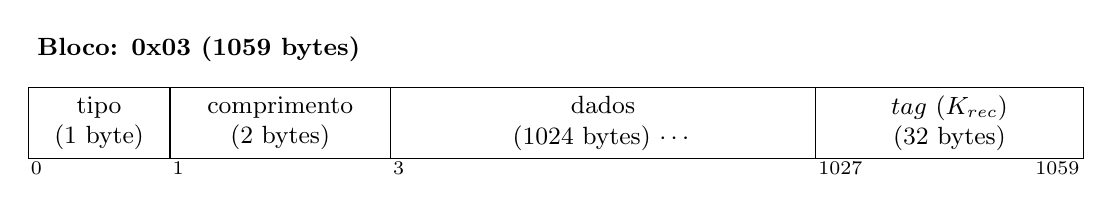
\begin{tikzpicture}[
		campo/.style={draw, minimum height=0.9cm, inner sep=1pt, font=\small, align=center},
		posini/.style={font=\scriptsize, anchor=north west, inner sep=1pt},
		posfim/.style={font=\scriptsize, anchor=north east, inner sep=1pt},
		titulo/.style={font=\small\bfseries, anchor=south west}
	]
		% \campo{x}{y}{largura}{texto}{posição inicial}
		\newcommand{\campo}[5]{%
			\node[campo, anchor=north west, minimum width=#3 cm] at (#1,#2) {#4};
			\node[posini] at (#1,#2-0.9) {#5};}
		% \fim{x}{y}{posição final}
		\newcommand{\fim}[3]{\node[posfim] at (#1,#2-0.9) {#3};}

		\node[titulo] at (0,0.2) {Bloco: 0x03 (1059 bytes)};
		\campo{0}{0}{1.8}{tipo\\(1 byte)}{0}
		\campo{1.8}{0}{2.8}{comprimento\\(2 bytes)}{1}
		\campo{4.6}{0}{5.4}{dados\\(1024 bytes) $\cdots$}{3}
		\campo{10.0}{0}{3.4}{$tag$ ($K_{rec}$)\\(32 bytes)}{1027}
		\fim{13.4}{0}{1059}
	\end{tikzpicture}
	\legend{Fonte: elaborado pelo autor.}
\end{figure}

A área de dados do bloco (figura \ref{fig:bloco-completo}), de até 1024 bytes, não é só registros: como mostra a figura \ref{fig:divisao-dados-bloco}, ela começa com o cabeçalho de 12 bytes do próprio
bloco, composto por $seq$ (4 bytes), $boot\_id$ (2 bytes), $t_{ms}$ inicial (4 bytes) e \textit{tamanho} (2 bytes), e só depois vêm os registros, em até 1012 bytes. É nesse cabeçalho que $seq$ fica: ele não é um
registro de medida, é o identificador de posição do bloco na sequência, usado para contar $HEAD_{seq}$ e para ordenar e detectar lacunas no servidor.

Os registros que seguem o cabeçalho são concatenados até o limite indicado pelo próprio campo \textit{tamanho}. Todo registro começa com \textit{tipo} (1 byte) e $\Delta t$ (2 bytes, deslocamento em
milissegundos a partir do $t_{ms}$ inicial do cabeçalho); o restante depende do \textit{tipo}. No caso de medida, cada leitura de PID ocupa 5 bytes (\textit{tipo}, $\Delta t$ e valor) e cada posição GPS
ocupa 15 bytes (\textit{tipo} 0xFF, $\Delta t$, latitude, longitude e altitude), e os registros se repetem até o bloco ser fechado. No caso de marcador, o bloco carrega um único registro de 11 bytes no
lugar das leituras: BOOT (\textit{tipo} 0xFE) ou LOSS (\textit{tipo} 0xFD), com $from\_seq$ e $to\_seq$ em vez do valor medido; o restante da área de 1024 bytes simplesmente não é escrito, pois o
\textit{tamanho} do bloco reflete só os 12 bytes do cabeçalho mais os 11 bytes do registro (seção \ref{sec:app-ble-dongle}).

\begin{figure}[H]
	\centering
	\caption{Divisão dos 1024 bytes da área de dados: cabeçalho do bloco e registros}
	\label{fig:divisao-dados-bloco}
	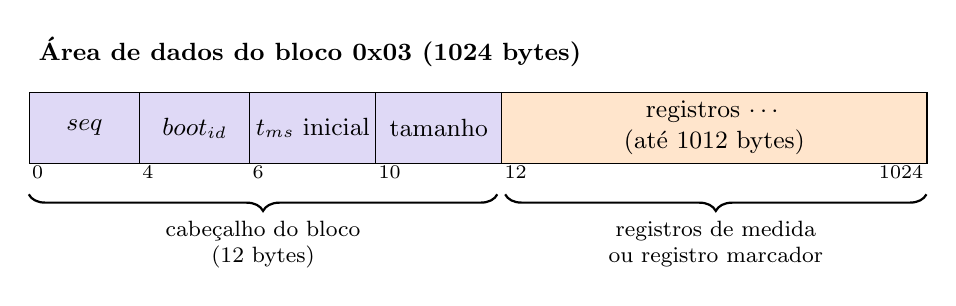
\begin{tikzpicture}[
		campo/.style={draw, minimum height=0.9cm, inner sep=1pt, font=\small, align=center},
		cabecalho/.style={campo, fill=blue!15},
		registros/.style={campo, fill=orange!20},
		posini/.style={font=\scriptsize, anchor=north west, inner sep=1pt},
		posfim/.style={font=\scriptsize, anchor=north east, inner sep=1pt},
		titulo/.style={font=\small\bfseries, anchor=south west}
	]
		% \campo{x}{y}{largura}{texto}{estilo}{posição inicial}
		\newcommand{\campo}[6]{%
			\node[#5, anchor=north west, minimum width=#3 cm] at (#1,#2) {#4};
			\node[posini] at (#1,#2-0.9) {#6};}
		% \fim{x}{y}{posição final}
		\newcommand{\fim}[3]{\node[posfim] at (#1,#2-0.9) {#3};}

		\node[titulo] at (0,0.2) {Área de dados do bloco 0x03 (1024 bytes)};
		\campo{0}{0}{1.4}{$seq$}{cabecalho}{0}
		\campo{1.4}{0}{1.4}{$boot_{id}$}{cabecalho}{4}
		\campo{2.8}{0}{1.6}{$t_{ms}$ inicial}{cabecalho}{6}
		\campo{4.4}{0}{1.6}{tamanho}{cabecalho}{10}
		\campo{6.0}{0}{5.4}{registros $\cdots$\\(até 1012 bytes)}{registros}{12}
		\fim{11.4}{0}{1024}

		\draw[decorate, decoration={brace, amplitude=6pt, mirror}, thick]
			(0,-1.3) -- (6.0-0.05,-1.3)
			node[midway, below=6pt, align=center, font=\footnotesize] {cabeçalho do bloco\\(12 bytes)};
		\draw[decorate, decoration={brace, amplitude=6pt, mirror}, thick]
			(6.0+0.05,-1.3) -- (11.4,-1.3)
			node[midway, below=6pt, align=center, font=\footnotesize] {registros de medida\\ou registro marcador};
	\end{tikzpicture}
	\legend{Fonte: elaborado pelo autor.}
\end{figure}

\begin{figure}[H]
	\centering
	\caption{Estrutura dos registros na área de dados: casos de medida e de marcador}
	\label{fig:registros-dados-bloco}
	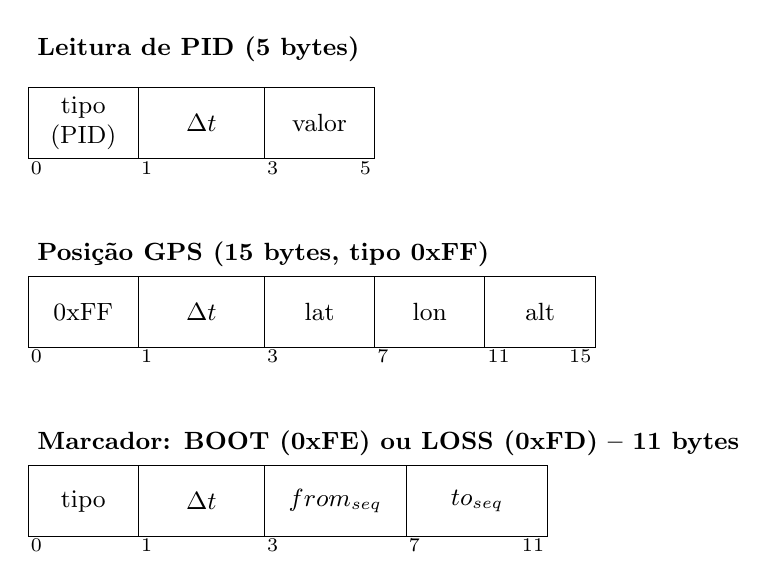
\begin{tikzpicture}[
		campo/.style={draw, minimum height=0.9cm, inner sep=1pt, font=\small, align=center},
		posini/.style={font=\scriptsize, anchor=north west, inner sep=1pt},
		posfim/.style={font=\scriptsize, anchor=north east, inner sep=1pt},
		titulo/.style={font=\small\bfseries, anchor=south west}
	]
		% \campo{x}{y}{largura}{texto}{posição inicial}
		\newcommand{\campo}[5]{%
			\node[campo, anchor=north west, minimum width=#3 cm] at (#1,#2) {#4};
			\node[posini] at (#1,#2-0.9) {#5};}
		% \fim{x}{y}{posição final}
		\newcommand{\fim}[3]{\node[posfim] at (#1,#2-0.9) {#3};}

		% Leitura de PID (caso de medida)
		\node[titulo] at (0,0.2) {Leitura de PID (5 bytes)};
		\campo{0}{0}{1.4}{tipo\\(PID)}{0}
		\campo{1.4}{0}{1.6}{$\Delta t$}{1}
		\campo{3.0}{0}{1.4}{valor}{3}
		\fim{4.4}{0}{5}

		% Posição GPS (caso de medida)
		\node[titulo] at (0,-2.4) {Posição GPS (15 bytes, tipo 0xFF)};
		\campo{0}{-2.4}{1.4}{0xFF}{0}
		\campo{1.4}{-2.4}{1.6}{$\Delta t$}{1}
		\campo{3.0}{-2.4}{1.4}{lat}{3}
		\campo{4.4}{-2.4}{1.4}{lon}{7}
		\campo{5.8}{-2.4}{1.4}{alt}{11}
		\fim{7.2}{-2.4}{15}

		% Marcador BOOT/LOSS (caso de marcador)
		\node[titulo] at (0,-4.8) {Marcador: BOOT (0xFE) ou LOSS (0xFD) -- 11 bytes};
		\campo{0}{-4.8}{1.4}{tipo}{0}
		\campo{1.4}{-4.8}{1.6}{$\Delta t$}{1}
		\campo{3.0}{-4.8}{1.8}{$from_{seq}$}{3}
		\campo{4.8}{-4.8}{1.8}{$to_{seq}$}{7}
		\fim{6.6}{-4.8}{11}
	\end{tikzpicture}
	\legend{Fonte: elaborado pelo autor.}
\end{figure}

O dongle mantém um cursor de envio, que é o próximo $seq$ a mandar ao app. A cada Pedido de Lote, ele envia a partir do cursor e o avança, mesmo que o ACK dos blocos anteriores ainda não tenha chegado.
Assim o app lê cada bloco logo depois de o dongle fechá-lo e o guarda no \textit{buffer}, e o envio ao servidor não precisa esperar a leitura pelo BLE. Se um POST falhar ou o servidor interromper um lote,
os blocos continuam no \textit{buffer} do app e são reenviados de lá, sem nova leitura. O cursor não tem prazo: ele só volta para $ACK_{seq} + 1$ no início de uma nova sessão ou quando o app manda um bloco
de erro (0x04 ou 0x07), porque nesses casos os blocos lidos podem ter se perdido. As regras do cursor estão na tabela \ref{tab:regras-cursor}. No fim, nada se perde, pois a \textit{flash} só é limpa quando
o ACK é recebido.

\begin{table}[H]
	\centering
	\caption{Regras do cursor de envio}
	\label{tab:regras-cursor}
	\begin{tabular}{|>{\raggedright\arraybackslash}m{0.32\textwidth}|>{\raggedright\arraybackslash}m{0.48\textwidth}|}
		\hline
		\textbf{Evento} & \textbf{Efeito no cursor} \\
		\hline
		Início de sessão (nova conexão BLE) & cursor $= ACK_{seq} + 1$ \\
		\hline
		Envio de um bloco ao app & O cursor avança 1 \\
		\hline
		Pedido de Lote & Envia do cursor até $\min(\text{cursor} + K - 1,\ HEAD_{seq})$ \\
		\hline
		ACK ou desafio com $ACK_{seq}$ maior & Libera a \textit{flash} até $ACK_{seq}$; cursor $= \max(\text{cursor},\ ACK_{seq} + 1)$ \\
		\hline
		Erro 0x04 ou 0x07 vindo do app & cursor $= ACK_{seq} + 1$ \\
		\hline
	\end{tabular}
\end{table}

\begin{figure}[H]
	\centering
	\caption{Cursor de envio e $ACK_{seq}$ na sequência de blocos do dongle}
	\label{fig:cursor-envio}
	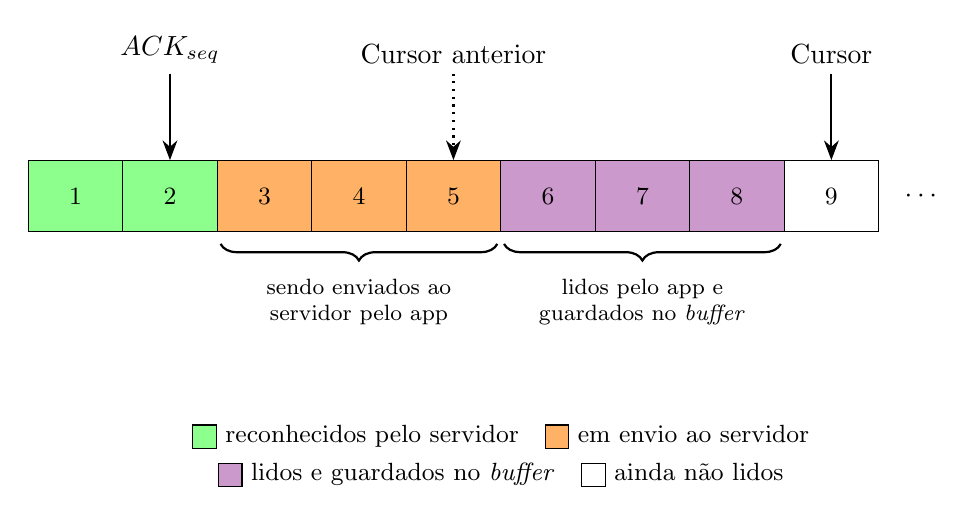
\begin{tikzpicture}[
			bloco/.style={draw, minimum width=1.2cm, minimum height=0.9cm, font=\small},
			ack/.style={bloco, fill=green!45},
			env/.style={bloco, fill=orange!60},
			prox/.style={bloco, fill=violet!40},
			pend/.style={bloco, fill=white},
			seta/.style={-{Stealth[length=2.5mm]}, thick}
		]
		\foreach \i/\est in {1/ack, 2/ack, 3/env, 4/env, 5/env, 6/prox, 7/prox, 8/prox, 9/pend} {
			\node[\est] (b\i) at (1.2*\i, 0) {\i};
		}
		\node[right=2mm of b9] {$\cdots$};

		% ACK_seq
		\draw[seta] ($(b2.north)+(0,1.1)$) -- (b2.north);
		\node[above] at ($(b2.north)+(0,1.1)$) {$ACK_{seq}$};

		% Cursor anterior (pontilhado)
		\draw[seta, dotted] ($(b5.north)+(0,1.1)$) -- (b5.north);
		\node[above] at ($(b5.north)+(0,1.1)$) {Cursor anterior};

		% Cursor atual
		\draw[seta] ($(b9.north)+(0,1.1)$) -- (b9.north);
		\node[above] at ($(b9.north)+(0,1.1)$) {Cursor};

		% Chave sobre os blocos em envio ao servidor
		\draw[decorate, decoration={brace, amplitude=6pt, mirror}, thick]
			($(b3.south west)+(0.05,-0.15)$) -- ($(b5.south east)+(-0.05,-0.15)$)
			node[midway, below=9pt, align=center, font=\footnotesize]
			{sendo enviados ao\\servidor pelo app};

		% Chave sobre os blocos lidos e no buffer
		\draw[decorate, decoration={brace, amplitude=6pt, mirror}, thick]
			($(b6.south west)+(0.05,-0.15)$) -- ($(b8.south east)+(-0.05,-0.15)$)
			node[midway, below=9pt, align=center, font=\footnotesize]
			{lidos pelo app e\\guardados no \textit{buffer}};

		% Legenda
		\node[font=\small, align=center] at (6.6,-3.3) {%
			\tikz[baseline=-0.5ex]\draw[fill=green!45] (0,-0.15) rectangle (0.3,0.15); reconhecidos pelo servidor\quad
			\tikz[baseline=-0.5ex]\draw[fill=orange!60] (0,-0.15) rectangle (0.3,0.15); em envio ao servidor\\[1mm]
			\tikz[baseline=-0.5ex]\draw[fill=violet!40] (0,-0.15) rectangle (0.3,0.15); lidos e guardados no \textit{buffer}\quad
			\tikz[baseline=-0.5ex]\draw[fill=white] (0,-0.15) rectangle (0.3,0.15); ainda não lidos};
	\end{tikzpicture}
	\legend{Fonte: elaborado pelo autor.}
\end{figure}

Na figura \ref{fig:cursor-envio}, os blocos 1 e 2 já foram reconhecidos pelo servidor, os blocos 3 a 5 estão sendo enviados ao servidor pelo app, e os blocos 6 a 8 já foram lidos pelo app e aguardam
no \textit{buffer} o próximo POST, com o cursor no bloco 9.
A figura \ref{fig:cursor-paralelismo} compara os dois comportamentos: sem \textit{buffer}, o dongle só transfere o lote seguinte depois do ACK do anterior; com \textit{buffer}, cada bloco é lido assim
que fecha, e o envio ao servidor acontece no ritmo de $T_{lat}$, independente da leitura.

\begin{figure}[H]
	\centering
	\caption{Paralelismo entre a leitura pelo BLE e o envio ao servidor, sem e com \textit{buffer} no app}
	\label{fig:cursor-paralelismo}
	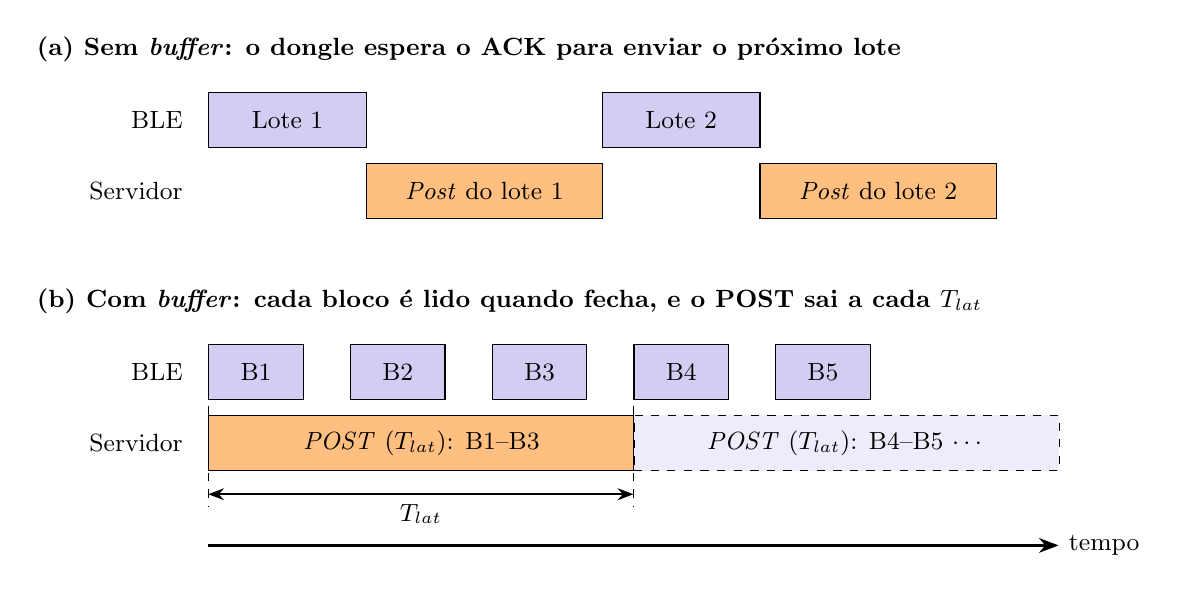
\begin{tikzpicture}[
			lane/.style={font=\small, anchor=east},
			ble/.style={draw, fill=blue!20, minimum height=0.7cm, anchor=west, font=\small, inner sep=0pt},
			post/.style={draw, fill=orange!50, minimum height=0.7cm, anchor=west, font=\small, inner sep=0pt},
			futuro/.style={draw, dashed, fill=blue!8, minimum height=0.7cm, anchor=west, font=\small, inner sep=0pt},
			titulo/.style={font=\small\bfseries, anchor=west},
			seta/.style={{Stealth[length=2mm]}-{Stealth[length=2mm]}, thick}
		]
		\def\tlbox#1#2#3#4#5{\node[#1, minimum width=#4cm] at (#2,#3) {#5};}

		% (a) sem buffer
		\node[titulo] at (-2.3,0.9) {(a) Sem \textit{buffer}: o dongle espera o ACK para enviar o próximo lote};
		\node[lane] at (-0.2,0) {BLE};
		\node[lane] at (-0.2,-0.9) {Servidor};
		\tlbox{ble}{0}{0}{2}{Lote 1}
		\tlbox{post}{2}{-0.9}{3}{\textit{Post} do lote 1}
		\tlbox{ble}{5}{0}{2}{Lote 2}
		\tlbox{post}{7}{-0.9}{3}{\textit{Post} do lote 2}

		% (b) com buffer: leituras curtas e independentes, POST periódico a cada T_lat
		\node[titulo] at (-2.3,-2.3) {(b) Com \textit{buffer}: cada bloco é lido quando fecha, e o POST sai a cada $T_{lat}$};
		\node[lane] at (-0.2,-3.2) {BLE};
		\node[lane] at (-0.2,-4.1) {Servidor};
		\tlbox{ble}{0}{-3.2}{1.2}{B1}
		\tlbox{ble}{1.8}{-3.2}{1.2}{B2}
		\tlbox{ble}{3.6}{-3.2}{1.2}{B3}
		\tlbox{ble}{5.4}{-3.2}{1.2}{B4}
		\tlbox{ble}{7.2}{-3.2}{1.2}{B5}
		\tlbox{post}{0}{-4.1}{5.4}{\textit{POST} ($T_{lat}$): B1--B3}
		\tlbox{futuro}{5.4}{-4.1}{5.4}{\textit{POST} ($T_{lat}$): B4--B5 $\cdots$}

		% Período T_lat
		\draw[dashed] (0,-3.0) -- (0,-4.9);
		\draw[dashed] (5.4,-3.0) -- (5.4,-4.9);
		\draw[seta] (0,-4.75) -- (5.4,-4.75);
		\node[font=\small, below] at (2.7,-4.75) {$T_{lat}$};

		% Eixo do tempo
		\draw[-{Stealth[length=2.5mm]}, thick] (0,-5.4) -- (10.8,-5.4) node[right, font=\small] {tempo};
	\end{tikzpicture}
	\legend{Fonte: elaborado pelo autor.}
\end{figure}

Os diagramas \ref{seq:aviso-novo-bloco} e \ref{seq:lote-envio} mostram esse processo de comunicação e troca de mensagens BLE entre dongle e app pelo serviço de SYNC.
O primeiro cobre o aviso de novo bloco e a decisão de \textit{handshake}, inclusive quando o app está sem conexão com a internet; o segundo cobre a leitura contínua, o \textit{buffer} no app
e o envio ao servidor.

\begin{figure}[H]
	\centering
	\caption{Diagrama de sequência do aviso de novo bloco e do \textit{handshake} com ou sem conexão}
	\label{seq:aviso-novo-bloco}
	% Fonte PlantUML: ../assets/aux-docs/plantuml/aquisicao-aviso-sequencia.puml
	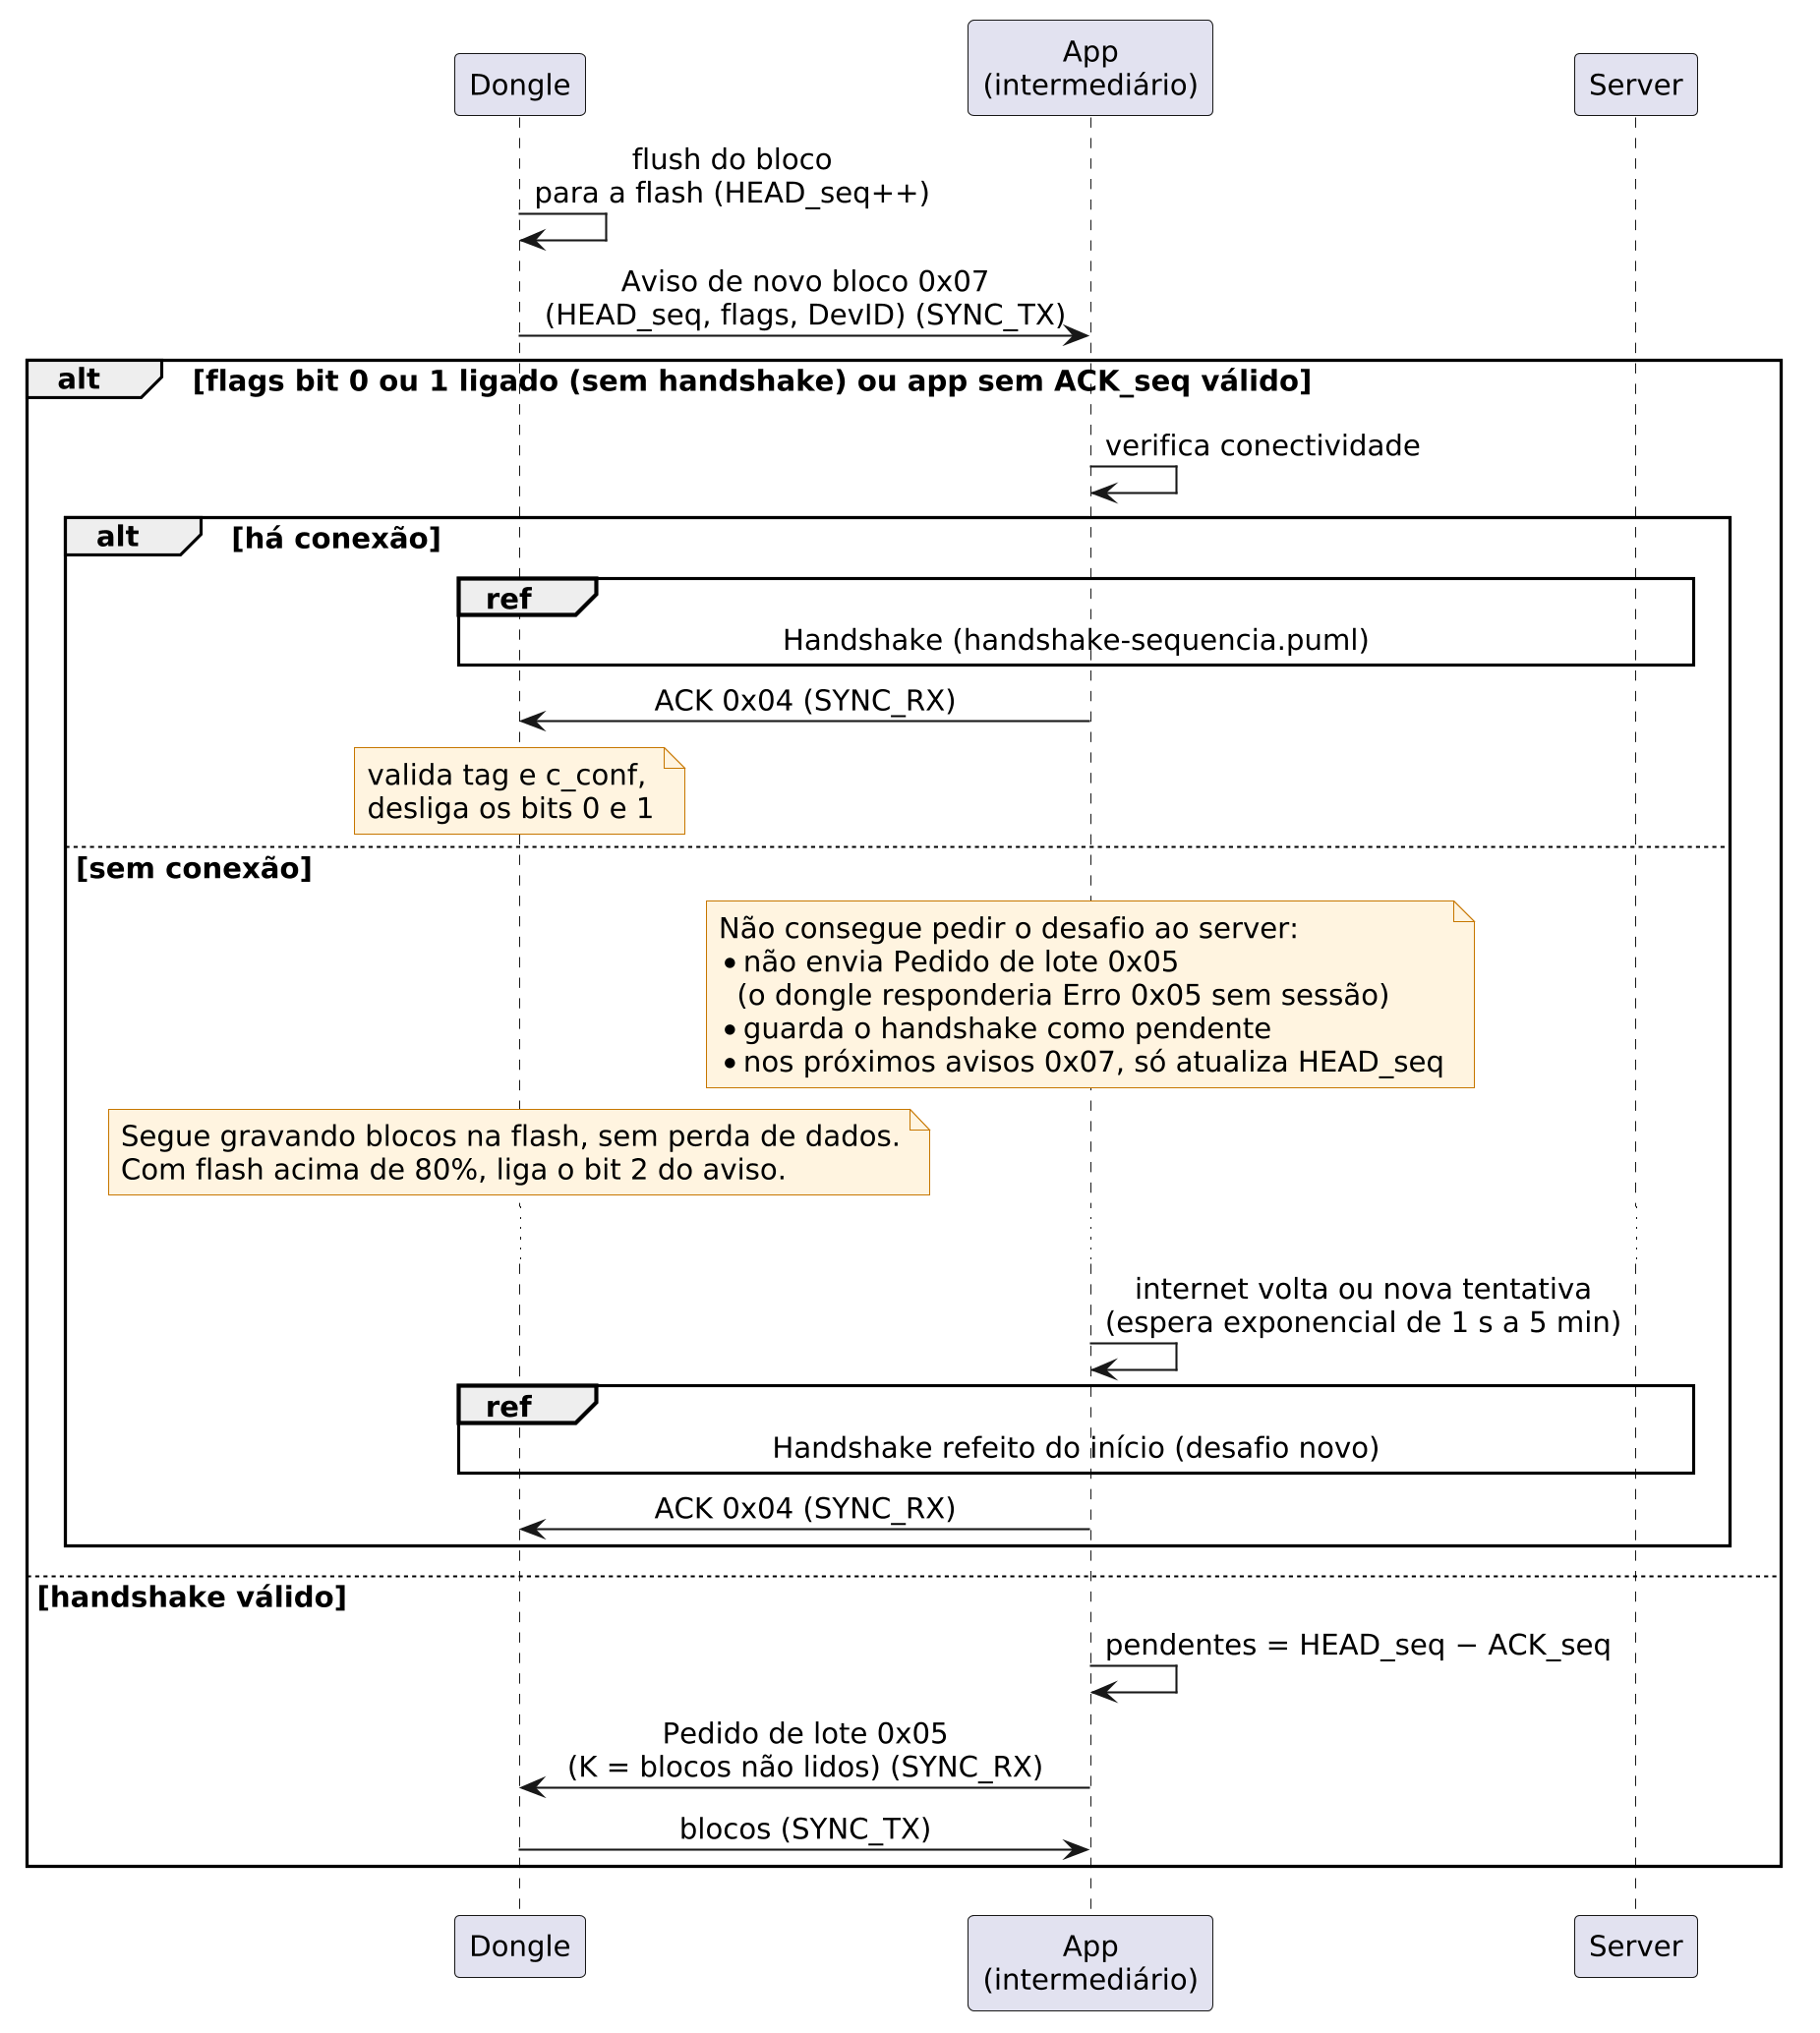
\includegraphics[width=\textwidth]{../../assets/aux-docs/aquisicao-aviso-sequencia.png}
	\legend{Fonte: elaborado pelo autor.}
\end{figure}

\begin{figure}[H]
	\centering
	\caption{Diagrama de sequência da leitura contínua, do \textit{buffer} no app e do envio ao servidor}
	\label{seq:lote-envio}
	% Fonte PlantUML: ../assets/aux-docs/plantuml/aquisicao-lote-sequencia.puml
	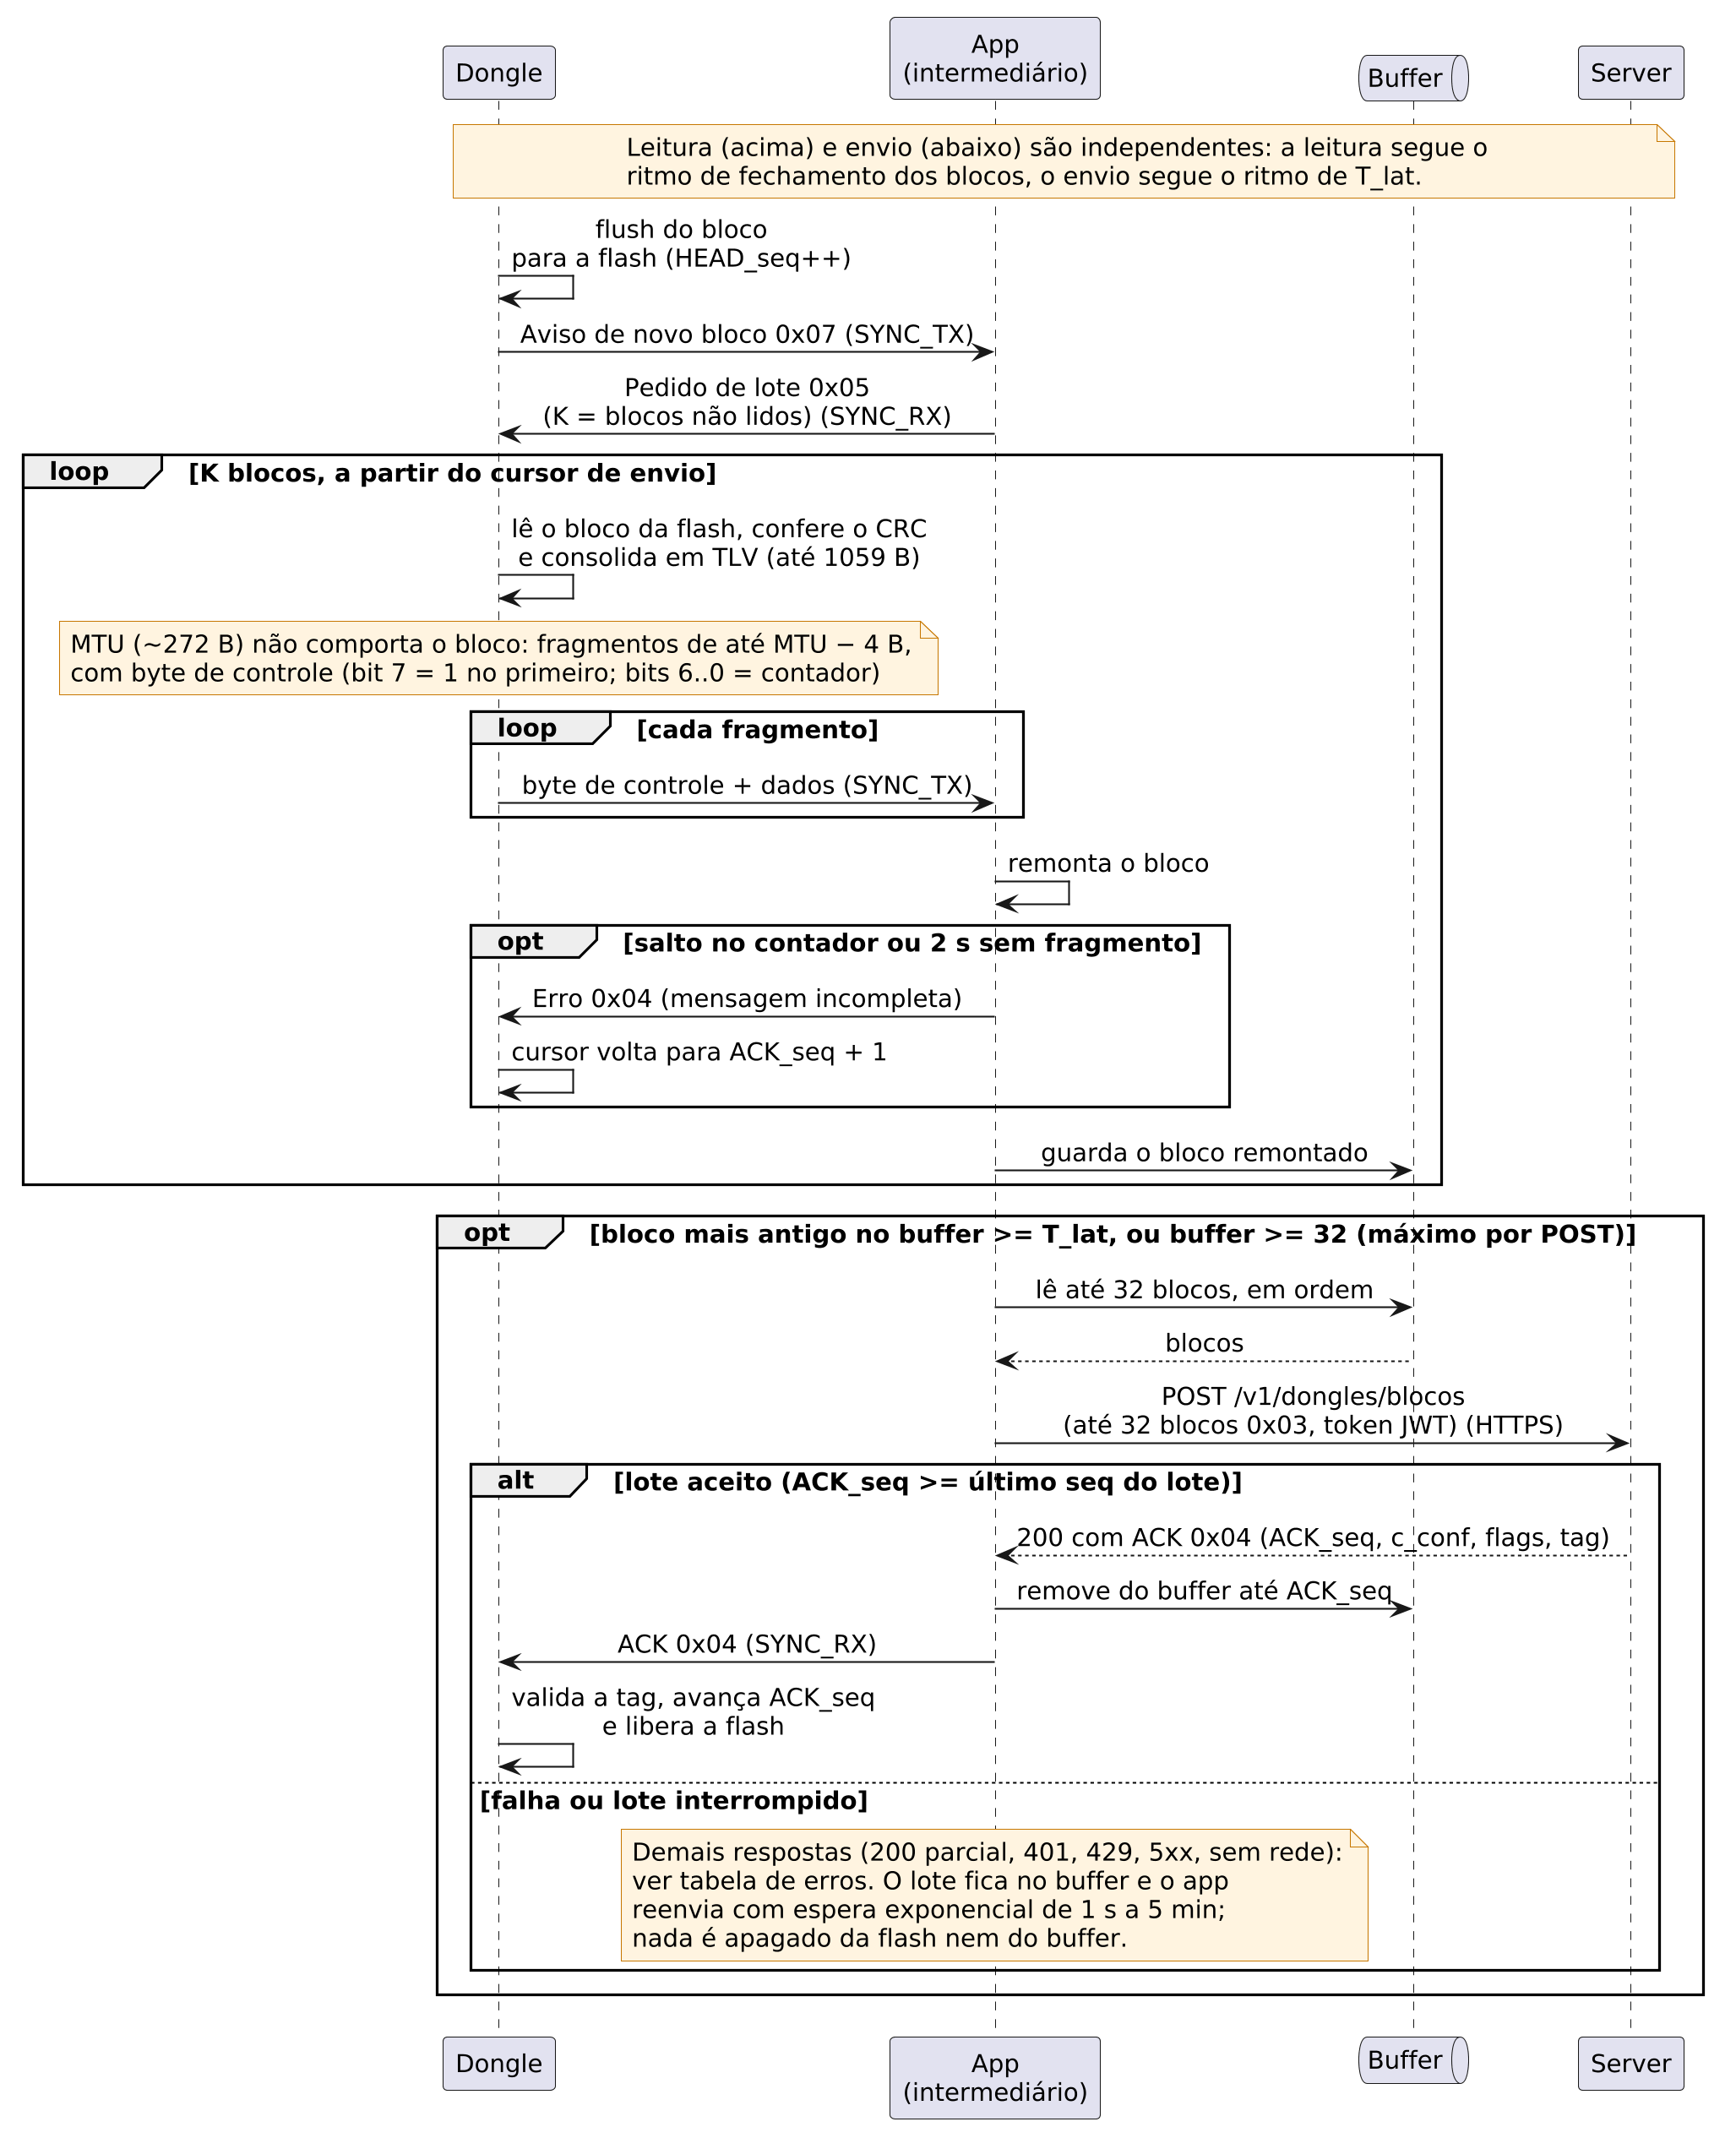
\includegraphics[width=\textwidth]{../../assets/aux-docs/aquisicao-lote-sequencia.png}
	\legend{Fonte: elaborado pelo autor.}
\end{figure}

\subsection{Ritmo de envio e \textit{buffer} no app} \label{subsec:ritmo-envio-buffer}

O envio dos blocos do app ao servidor é controlado por um único parâmetro de latência, $T_{lat}$, que define quanto tempo, no máximo, um bloco lido pode esperar no \textit{buffer} do app antes de ser
enviado. Ele permite trocar latência por consumo de bateria do celular e por carga no servidor, sem mudar o dongle, o servidor ou o formato das mensagens. Os parâmetros são mostrados na tabela
\ref{tab:params-buffer}.

\begin{table}[H]
	\centering
	\caption{Parâmetros do envio com \textit{buffer} no app}
	\label{tab:params-buffer}
	\begin{tabular}{|>{\raggedright\arraybackslash}m{0.2\textwidth}|>{\raggedright\arraybackslash}m{0.52\textwidth}|>{\centering\arraybackslash}m{0.16\textwidth}|}
		\hline
		\textbf{Parâmetro} & \textbf{Significado} & \textbf{Padrão} \\
		\hline
		$T_{lat}$ & Tempo máximo que um bloco espera no \textit{buffer} antes de ser enviado & 60 s (de 10 a 300 s) \\
		\hline
		$B_{max}$ & Máximo de blocos no \textit{buffer} do app & 64 (ao menos o dobro do máximo de 32 blocos aceito por POST) \\
		\hline
		Espera entre tentativas & Após falha de rede ou 5xx & Exponencial de 1 s a 5 min \\
		\hline
	\end{tabular}
\end{table}

O app avalia a regra de envio a cada segundo e sempre que chega um aviso, um bloco ou um ACK. Se não houver POST em andamento e o \textit{buffer} não estiver vazio, ele envia quando o bloco mais antigo
completar $T_{lat}$ desde o seu aviso, ou quando o \textit{buffer} acumular os 32 blocos aceitos por POST, limite fixado pelo servidor (tabela \ref{tab:erros-bloco}, erro 429). O segundo caso ocorre
quando há atraso acumulado: os lotes de 32 saem em sequência, sem esperar $T_{lat}$. Antes de cada POST, se o token estiver ausente ou a menos de 5 minutos de expirar, o app faz um novo \textit{handshake}. Ao receber o ACK, o app remove do \textit{buffer} os blocos até
$ACK_{seq}$, escreve o ACK no dongle e volta a ler os blocos disponíveis. Se o \textit{buffer} chegar a $B_{max}$, o app para de ler até um ACK liberar espaço, e os blocos continuam seguros na
\textit{flash} do dongle.

Em regime, com conexão disponível, nenhum bloco espera mais do que o tempo da equação \ref{eq:latencia-max}:

\begin{equation} \label{eq:latencia-max}
	L_{max} = T_{bloco} + T_{lat} + t_{envio}
\end{equation}

em que $T_{bloco} = 10$ s é o tempo máximo de fechamento de um bloco e $t_{envio}$ é a ida e volta do POST. Reduzir $T_{lat}$ abaixo de cerca de 10 s não ajuda, porque o limite passa a ser o fechamento
do bloco. A tabela \ref{tab:efeito-tlat} mostra o efeito esperado de diferentes valores.

\begin{table}[H]
	\centering
	\caption{Efeito de $T_{lat}$ no envio (um bloco a cada 6 a 10 s; servidor com 10 mil dongles)}
	\label{tab:efeito-tlat}
	\begin{tabular}{|>{\centering\arraybackslash}m{0.1\textwidth}|>{\centering\arraybackslash}m{0.18\textwidth}|>{\centering\arraybackslash}m{0.18\textwidth}|>{\centering\arraybackslash}m{0.14\textwidth}|>{\centering\arraybackslash}m{0.22\textwidth}|}
		\hline
		\textbf{$T_{lat}$} & \textbf{Blocos por POST} & \textbf{POSTs por minuto} & \textbf{$L_{max}$} & \textbf{Requisições por segundo no servidor} \\
		\hline
		10 s & 1 a 2 & 6 & cerca de 20 s & cerca de 1.000 \\
		\hline
		30 s & 3 a 5 & 2 & cerca de 40 s & cerca de 330 \\
		\hline
		60 s & 6 a 10 & 1 & cerca de 70 s & cerca de 170 \\
		\hline
		120 s & 12 a 20 & 0,5 & cerca de 130 s & cerca de 85 \\
		\hline
	\end{tabular}
\end{table}

Para o TCC e o \textit{benchmark}, $T_{lat}$ é uma configuração local do app, com padrão de 60 s. Numa versão comercial, o servidor pode devolvê-lo junto com o token na resposta ao desafio, e o mínimo
é reforçado pelo limite de taxa por DevId. Em qualquer caso, $T_{lat}$ altera apenas quando os dados chegam ao servidor, nunca se chegam ou se são aceitos: o dongle só apaga um bloco com o ACK, o
servidor só aceita blocos em ordem e o app nunca altera os bytes de um bloco.

\section{Implementação do servidor}

O servidor será um VPS com uma API em GoLang que responderá as requisições de desafio para o dongle feitas pelo app, processará e validará
as respostas desses desafios, e também receberá os blocos de dados medidos pelo dongle vindos do app. A ideia de usar GoLang é permitir 
rápido processamento das requisições e capacidade maior de carga de requisições.

A tabela \ref{table:endpoints-api} resume os endpoints da API, quando o app os chama, e o que cada um recebe e devolve. No sentido dongle
$\rightarrow$ servidor, tudo é assinado pelo dongle: blocos e respostas a desafios. No sentido servidor $\rightarrow$ dongle, tudo é assinado
pelo servidor: desafio, confirmação de recebimento e token de diagnóstico. O app apenas transporta os bytes; a autenticação do app no
servidor serve para identificar o usuário e limitar abusos, nunca para dar confiança aos dados.

\begin{longtable}{|>{\raggedright\arraybackslash}p{0.23\textwidth}|>{\raggedright\arraybackslash}p{0.16\textwidth}|>{\raggedright\arraybackslash}p{0.27\textwidth}|>{\raggedright\arraybackslash}p{0.24\textwidth}|}
	\caption{Endpoints da API (/v1/dongles)}
	\label{table:endpoints-api} \\
	\hline
	\textbf{Endpoint} & \textbf{Quando o app chama} & \textbf{Entrada} & \textbf{Saída} \\
	\hline
	\endfirsthead
	\hline
	\textbf{Endpoint} & \textbf{Quando o app chama} & \textbf{Entrada} & \textbf{Saída} \\
	\hline
	\endhead
	\hline
	\endfoot
	POST \texttt{/\{id\}/desafio} & Ao conectar com internet; o dongle pede o desafio & $DevId$, informado pelo app, sem autenticação & Desafio 0x01: $c_S$, $N_S$ e tag $K_{auth}$ \\
	\hline
	POST \texttt{/\{id\}/desafio} \newline \texttt{/resposta} & Ao dongle responder & Resposta 0x02: $c_S$, $N_S$, $TAIL_{seq}$, $HEAD_{seq}$, $boot\_id$, $t_{ms}$ e tag $K_{auth}$ & ACK 0x04 com $ACK_{seq}$ e o token JWT \\
	\hline
	POST \texttt{/blocos} & Em lotes, a partir da última confirmação & Lote de blocos assinados; $DevId$ identificado pelo token JWT, não pela URL & Confirmação assinada com $seq\_contiguo$ \\
	\hline
	GET \texttt{/\{id\}/confirmacao} & Ao reconectar, antes de enviar & --- & A confirmação assinada mais recente \\
\end{longtable}

Os corpos são em binário (\textit{application/octet-stream}), repassados pelo app sem conversão: converter para JSON no app abriria espaço
para alterações e custaria CPU no servidor. As respostas de erro seguem a convenção: \texttt{400} para lote malformado, \texttt{422} para
assinatura inválida (o bloco vai para a tabela de rejeitados), \texttt{409} para nonce já usado ou expirado e \texttt{503} com
\texttt{Retry-After} sob sobrecarga.

O banco de dados será PostgreSQL, com TimescaleDB e PostGIS para armazenar os dados de telemetria e localização, respectivamente.

Para simplificar, no mesmo VPS, mas com configurações de acesso mais restritas, estará um servidor KMS usando HashiCorp Vault para gerenciar as
chaves usadas nos HMACs de autenticação e de blocos de dados ($K_{auth}$ e $K_{rec}$, respectivamente), e também a chave privada para assinar os
tokens JWT que permitirão que o app envie blocos de maneira autenticada, evitando possível sobrecarga no endpoint de recebimento de blocos. 

\subsection{Estrutura de dados}

Os dados passam por camadas, da evidência bruta até as leituras já decodificadas, de modo que cada camada possa ser reconstruída a
partir da anterior. A camada bronze guarda exatamente o que foi recebido, sem decodificar nada: a tabela \texttt{bloco\_bruto} tem
chave primária $(dongle\_id, seq)$, o que neutraliza tanto a repetição quanto a reordenação de blocos diretamente no banco, e a tabela
\texttt{dongle\_estado} guarda o estado operacional de cada dongle visto pelo servidor: o maior \textit{seq} contíguo já confirmado
($seq\_contiguo$), o maior \textit{seq} já visto, a faixa $[TAIL_{seq}, HEAD_{seq}]$ que o dongle ainda guarda na \textit{flash}
segundo o último \textit{handshake} aceito, e o contador $ultimo\_c\_S$ usado para emitir desafios com $c_S$ estritamente crescente.
A \autoref{fig:modelo-bronze} mostra essas duas tabelas.

\begin{figure}[H]
	\centering
	\caption{Modelo de dados da camada bronze}
	\label{fig:modelo-bronze}
	% Fonte PlantUML: ../assets/aux-docs/plantuml/modelo-dados-bronze.puml
	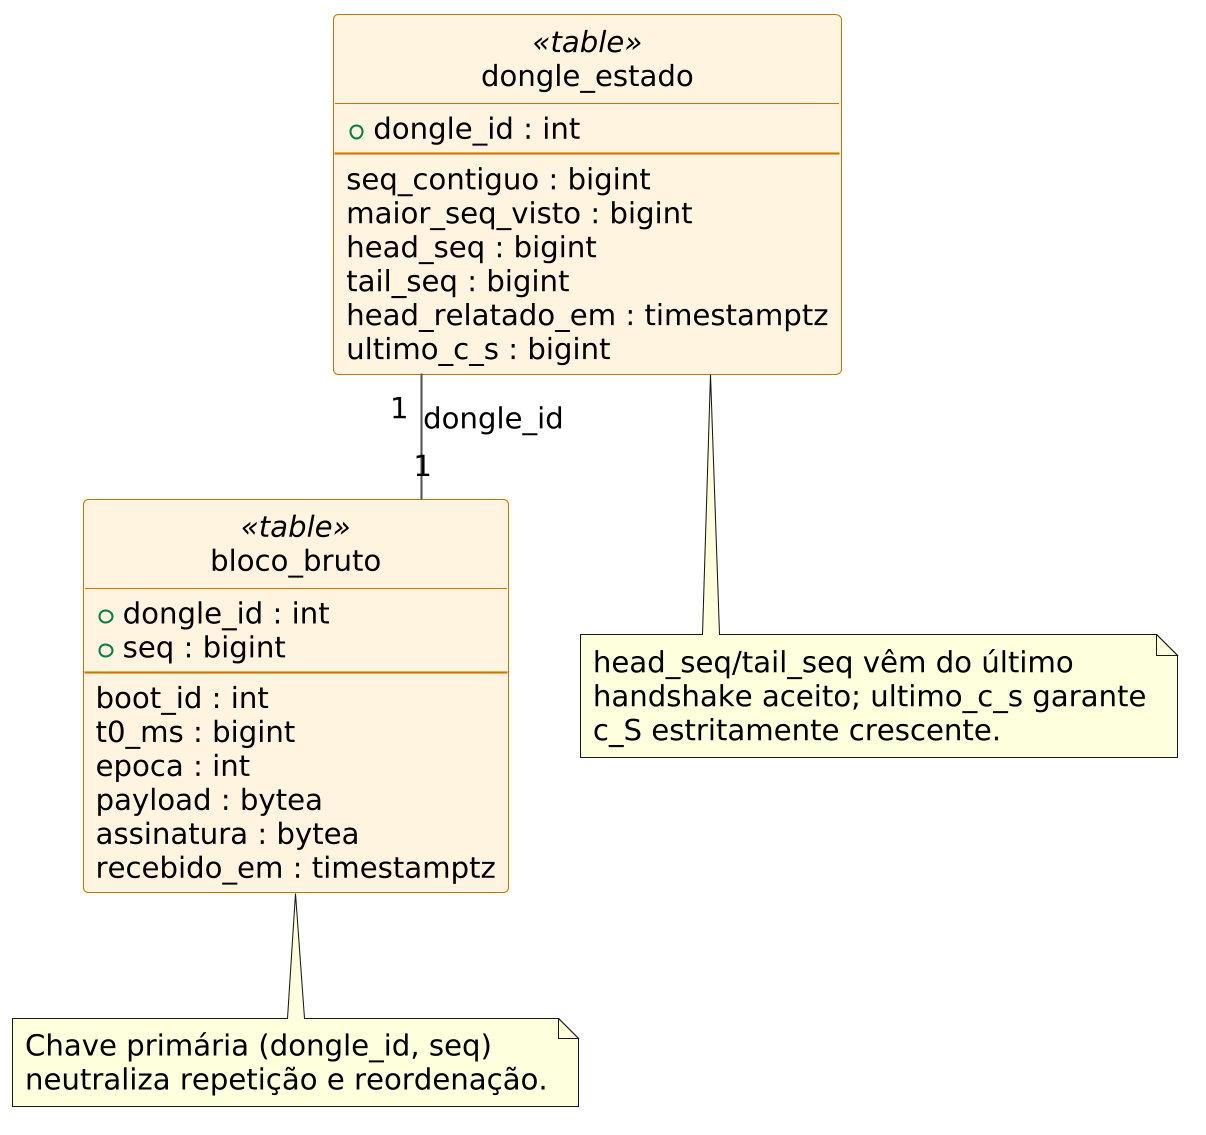
\includegraphics[width=0.75\textwidth]{../../assets/aux-docs/modelo-dados-bronze.png}
	\legend{Fonte: elaborado pelo autor.}
\end{figure}

A camada de contexto guarda os \textit{boots} e o rastro de cada \textit{handshake}. A tabela \texttt{boot} tem uma linha por
\textit{boot}, com a configuração vigente e a reta de tempo (recalculada pelo worker). A tabela \texttt{desafio} guarda todo desafio
emitido, respondido ou não, identificado por $(dongle\_id, c_S)$, com os campos trazidos pela Resposta 0x02 ($boot\_id$, $t\_ms$,
$HEAD_{seq}$, $TAIL_{seq}$), o resultado do \textit{handshake} e os efeitos de um \textit{handshake} aceito: $ACK_{seq}$ e o identificador
do JWT emitido ($token\_jti$). Uma tabela de lacunas declaradas, \texttt{lacuna}, guarda $DevId$, $from\_seq$, $to\_seq$, causa (BOOT, LOSS
ou OVERFLOW), instante do registro e o $c_S$ do \textit{handshake} ou o $seq$ do bloco que a declarou, cobrindo tanto a perda detectada no
\textit{handshake} (OVERFLOW) quanto a declarada pelos blocos marcadores BOOT e LOSS na ingestão. A tabela \texttt{ancora\_tempo} guarda
apenas as medições com $S_2 - S_1 \leq 2$ s, cada uma referenciando o nonce do desafio que a gerou. A \autoref{fig:modelo-contexto}
mostra essas três tabelas.

\begin{figure}[H]
	\centering
	\caption{Modelo de dados da camada de contexto}
	\label{fig:modelo-contexto}
	% Fonte PlantUML: ../assets/aux-docs/plantuml/modelo-dados-contexto.puml
	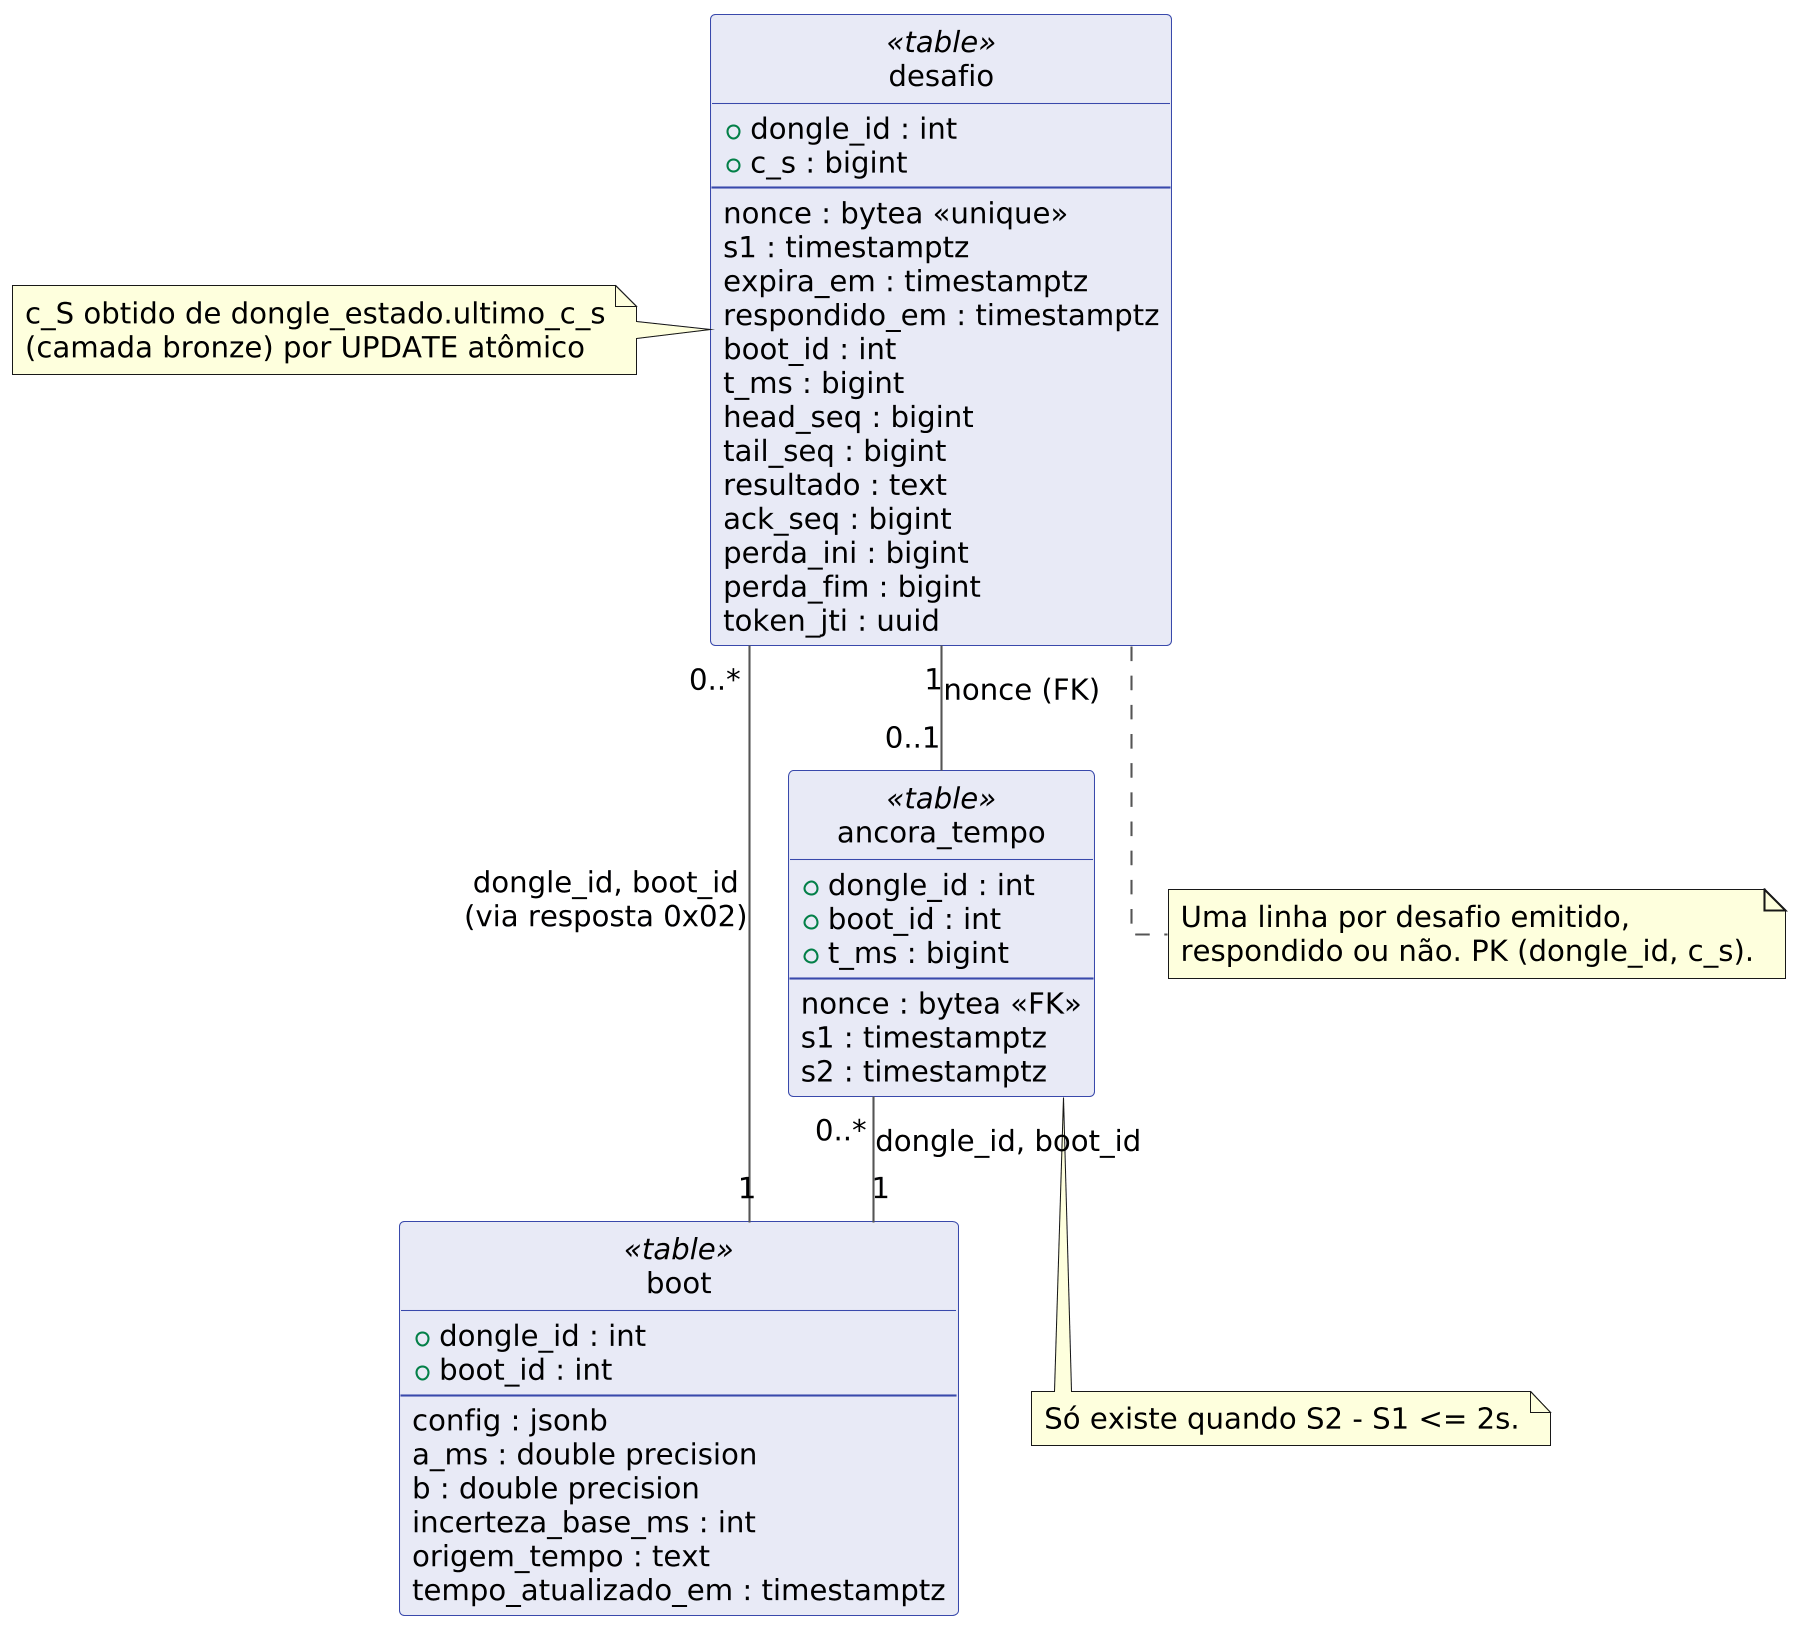
\includegraphics[width=\textwidth]{../../assets/aux-docs/modelo-dados-contexto.png}
	\legend{Fonte: elaborado pelo autor.}
\end{figure}

A camada silver guarda as leituras já decodificadas. A tabela \texttt{pid} é a fonte da verdade de como decodificar cada PID (fator,
deslocamento e faixa válida), carregada em memória pela API para decodificar cada leitura sem fórmulas fixas no código. As tabelas
\texttt{leitura} e \texttt{posicao} são \textit{hypertables} do TimescaleDB, particionadas por \texttt{recebido\_em}, com índice em
$(dongle\_id, boot\_id, t\_ms)$ para consultas por viagem. A \autoref{fig:modelo-silver} mostra essas três tabelas.

\begin{figure}[H]
	\centering
	\caption{Modelo de dados da camada silver}
	\label{fig:modelo-silver}
	% Fonte PlantUML: ../assets/aux-docs/plantuml/modelo-dados-silver.puml
	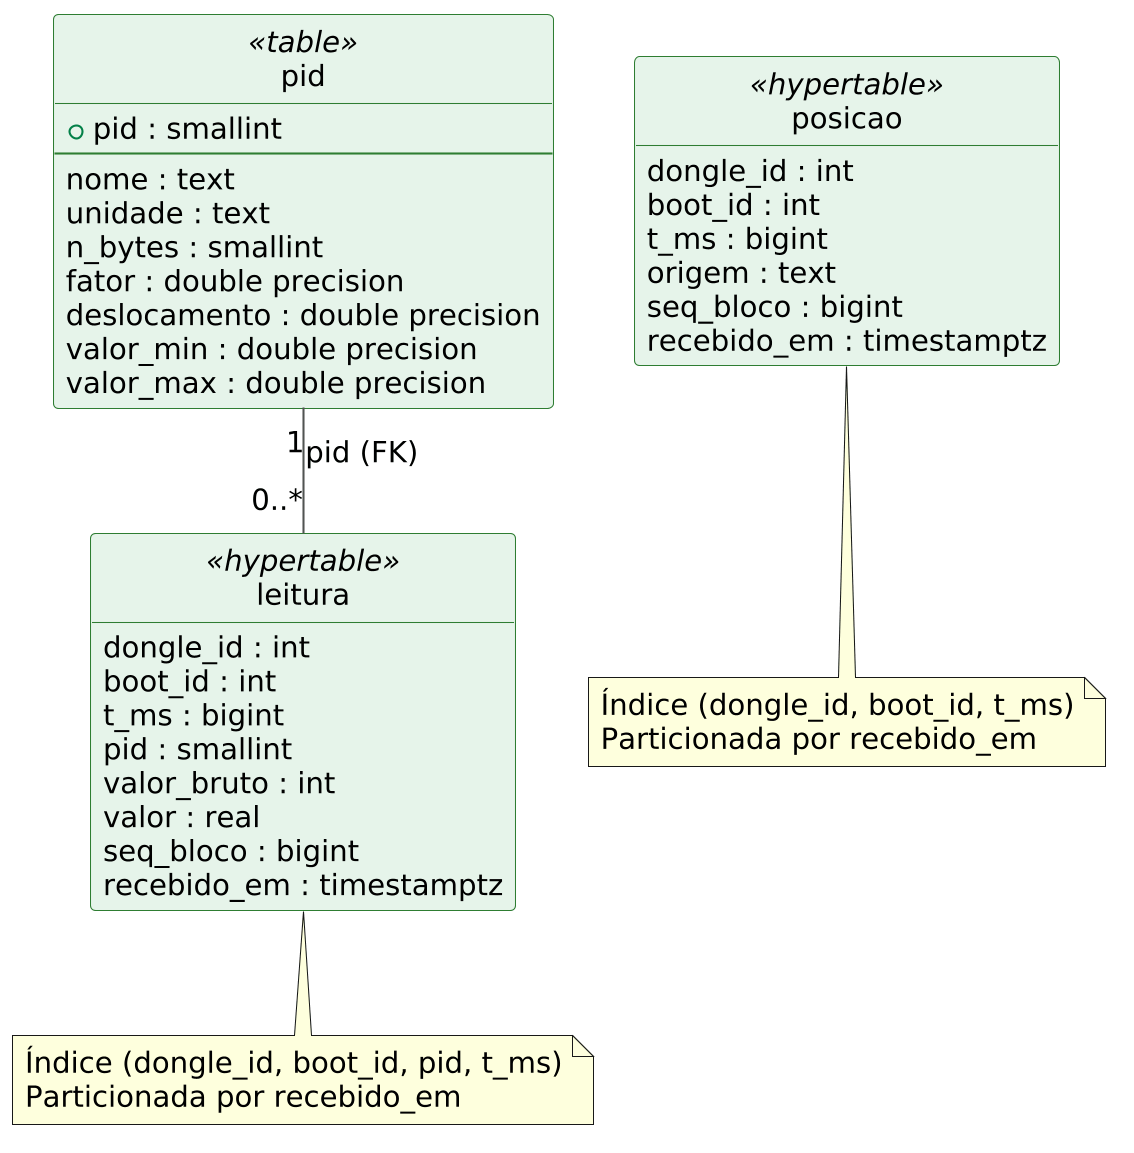
\includegraphics[width=0.85\textwidth]{../../assets/aux-docs/modelo-dados-silver.png}
	\legend{Fonte: elaborado pelo autor.}
\end{figure}

\subsection{Ingestão de um lote}

O custo de escala do servidor está na escrita no banco, não na verificação de assinaturas nem na decodificação dos blocos. Por isso, a
ingestão processa um lote inteiro por transação, em vez de um bloco por vez, o que divide o custo do \textit{commit} por dezenas de
blocos. O fluxo segue os passos descritos na \autoref{fig:ingestao-lote-servidor}: o lote chega, as assinaturas são verificadas em
paralelo, blocos inválidos vão para a tabela de rejeitados, e os blocos válidos são inseridos em \texttt{bloco\_bruto} com
\texttt{ON CONFLICT DO NOTHING}, o que torna a ingestão idempotente, já que o dongle reenvia a partir do último ACK. Como cada dongle
tem seus blocos travados por um \texttt{pg\_advisory\_xact\_lock}, lotes do mesmo dongle ficam em série, mas dongles diferentes seguem
em paralelo. Quando um bloco é o marcador BOOT ou LOSS, a mesma transação grava a lacuna declarada na tabela \texttt{lacuna} com a causa
correspondente, sem gerar linhas nas tabelas de PID e de posições. Ao final, a API atualiza $seq\_contiguo$ e $maior\_seq\_visto$ em
\texttt{dongle\_estado}, avançando também $HEAD_{seq}$ caso algum bloco novo tenha $seq$ maior que o salvo.

\begin{figure}[H]
	\centering
	\caption{Diagrama de sequência da ingestão de um lote de blocos}
	\label{fig:ingestao-lote-servidor}
	% Fonte PlantUML: ../assets/aux-docs/plantuml/ingestao-lote-servidor.puml
	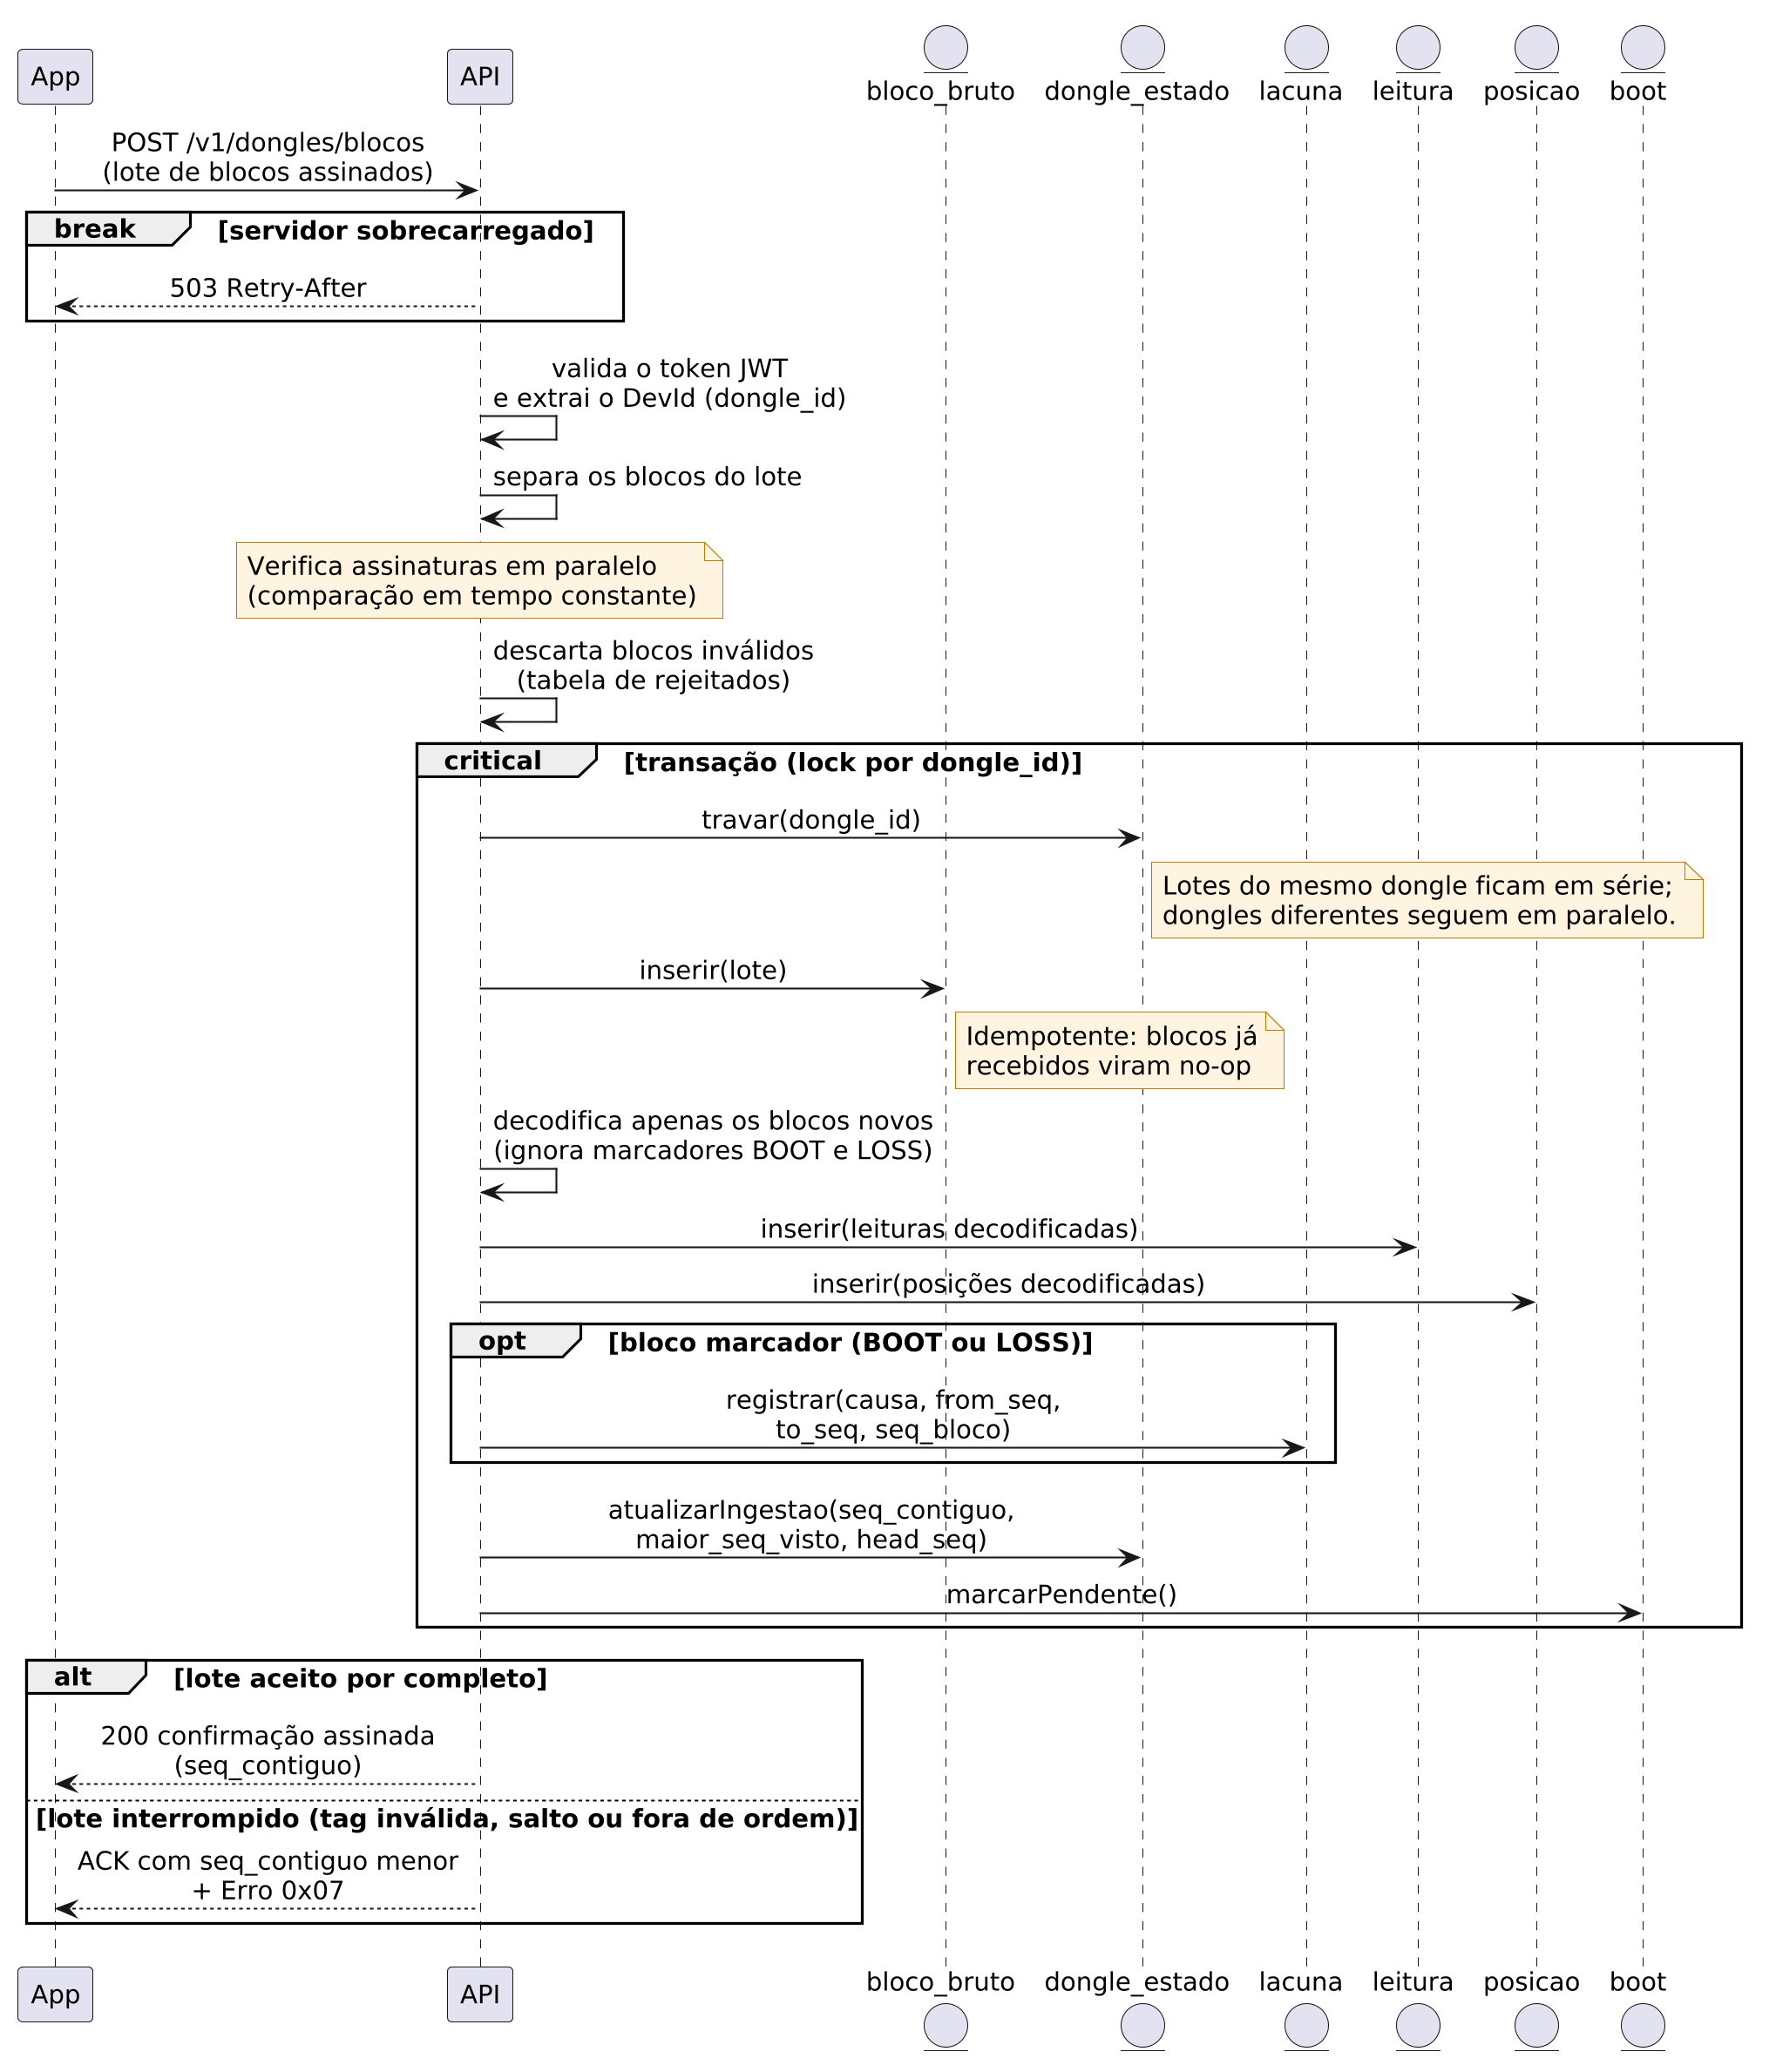
\includegraphics[width=\textwidth]{../../assets/aux-docs/ingestao-lote-servidor.png}
	\legend{Fonte: elaborado pelo autor.}
\end{figure}

\subsection{Handshake}

Do lado do servidor, o \textit{handshake} são duas requisições do app, com o estado guardado entre elas na tabela \texttt{desafio}, como
mostram as \autoref{fig:handshake-servidor-desafio} (pedido de desafio), \autoref{fig:handshake-servidor-resposta} (resposta do dongle)
e \autoref{fig:handshake-servidor-worker} (processamento assíncrono disparado ao final da segunda). Ele serve a quatro propósitos: provar
que a resposta do dongle é nova, por meio de $c_S$ e
$N_S$; medir a âncora de tempo do boot, a partir de $S_1$, $S_2$ e do $t\_ms$ do dongle; receber $HEAD_{seq}$ e $TAIL_{seq}$ atestados
pelo dongle; e emitir o token JWT que autoriza o envio de blocos. Desafio, resposta e ACK são autenticados com $K_{auth}$.

No \texttt{POST /v1/dongles/\{id\}/desafio}:

\begin{enumerate}
	\item O servidor lê o $DevId$ informado pelo app. O pedido não é autenticado, porque o JWT ainda não existe; isso é seguro, pois
	apenas o dongle com $K_{auth}$ consegue responder ao desafio.
	\item A taxa é limitada por $DevId$: se ele já pediu desafios demais no último minuto, o servidor responde \texttt{429}, evitando
	que um app malicioso encha a tabela \texttt{desafio}.
	\item O servidor obtém $c_S$ com um \texttt{UPDATE} atômico sobre $ultimo\_c\_S$ em \texttt{dongle\_estado}, mantendo-o
	estritamente crescente mesmo com pedidos simultâneos; o dongle recusa um desafio cujo $c_S$ não seja maior que o último aceito.
	\item É gerado $N_S$ com 16 bytes aleatórios (\texttt{crypto/rand}).
	\item O servidor anota $S_1$, insere a linha em \texttt{desafio} e responde o Desafio 0x01 ($c_S$, $N_S$ e tag $K_{auth}$).
\end{enumerate}

No \texttt{POST /v1/dongles/\{id\}/desafio/resposta}:

\begin{enumerate}
	\item O servidor anota $S_2$ assim que a requisição chega, antes de qualquer outro processamento.
	\item Lê a Resposta 0x02 ($c_S$, $N_S$, $TAIL_{seq}$, $HEAD_{seq}$, $boot\_id$, $t\_ms$) e verifica a tag com o $K_{auth}$ do
	dongle; se for inválida, marca o desafio como \texttt{tag\_invalida} e responde \texttt{422}.
	\item Consome o desafio com um \texttt{UPDATE} que confere, numa única instrução, se ele pertence àquele dongle, está pendente e
	dentro do prazo, impedindo duas respostas simultâneas ao mesmo desafio; se nenhuma linha voltar, responde \texttt{409}.
	\item Confere a consistência: $TAIL_{seq}$ de até $HEAD_{seq} + 1$ e $HEAD_{seq}$ não menor que o valor salvo. Se falhar, marca
	como \texttt{inconsistente} e responde \texttt{422}.
	\item Confere se $S_2 - S_1$ é de até 2 s. Se for maior, o \textit{handshake} segue, mas sem âncora: o desafio fica como
	\texttt{aceito\_sem\_ancora}, e o ACK pede um novo desafio.
	\item Abre uma transação e toma \texttt{pg\_advisory\_xact\_lock(dongle\_id)}. Aplica a regra do $TAIL_{seq}$: se
	$TAIL_{seq} > seq\_contiguo + 1$, os blocos entre $seq\_contiguo + 1$ e $TAIL_{seq} - 1$ foram descartados pelo dongle com a
	\textit{flash} cheia, e a faixa exata é gravada na tabela \texttt{lacuna} com causa OVERFLOW, avançando $seq\_contiguo$ para $TAIL_{seq} - 1$.
	Em seguida, atualiza $HEAD_{seq}$, $TAIL_{seq}$ e $head\_relatado\_em$ em \texttt{dongle\_estado}, grava a âncora em
	\texttt{ancora\_tempo} quando houver, cria a linha de \texttt{boot} se ainda não existir e marca o boot como pendente para o
	worker.
	\item Faz o \textit{commit}, avisa o worker com \texttt{NOTIFY}, emite o JWT ($sub = DevId$, com o $jti$ gravado em
	\texttt{desafio}) e responde o ACK 0x04 com o $ACK_{seq}$ resultante, a tag $K_{auth}$, o token e, opcionalmente, o valor de
	$T_{lat}$ a ser usado na sessão (seção \ref{subsec:ritmo-envio-buffer}).
\end{enumerate}

$S_1$ e $S_2$ vêm do relógio da API (\texttt{time.Now()}), sincronizado por NTP, e não do \texttt{now()} do PostgreSQL, que devolve o
início da transação e poderia atrasar a medida. $S_1$ é anotado antes do \texttt{INSERT}, um pouco antes de a resposta sair, o que só
alarga o intervalo $[S_1, S_2]$ e deixa a âncora mais conservadora, nunca errada; $S_2$ é anotado na chegada pelo mesmo motivo, para
que o tempo gasto verificando a assinatura não entre na medida.

O pedido de desafio não toma o \textit{lock} do dongle, mas o passo 6 da resposta toma, porque a regra do $TAIL_{seq}$ pode avançar
$seq\_contiguo$ e essa mudança não pode se misturar com um lote do mesmo dongle sendo gravado ao mesmo tempo. Como o $TAIL_{seq}$ é
autenticado com $K_{auth}$ e amarrado a $N_S$, o app não consegue forjar uma perda; ele pode provocá-la deixando de pedir lotes
(A3.2), mas a perda chega ao servidor declarada, com a faixa exata.

\begin{figure}[H]
	\centering
	\caption{Diagrama de sequência do \textit{handshake} no servidor: \texttt{POST /desafio}}
	\label{fig:handshake-servidor-desafio}
	% Fonte PlantUML: ../assets/aux-docs/plantuml/handshake-servidor-desafio.puml
	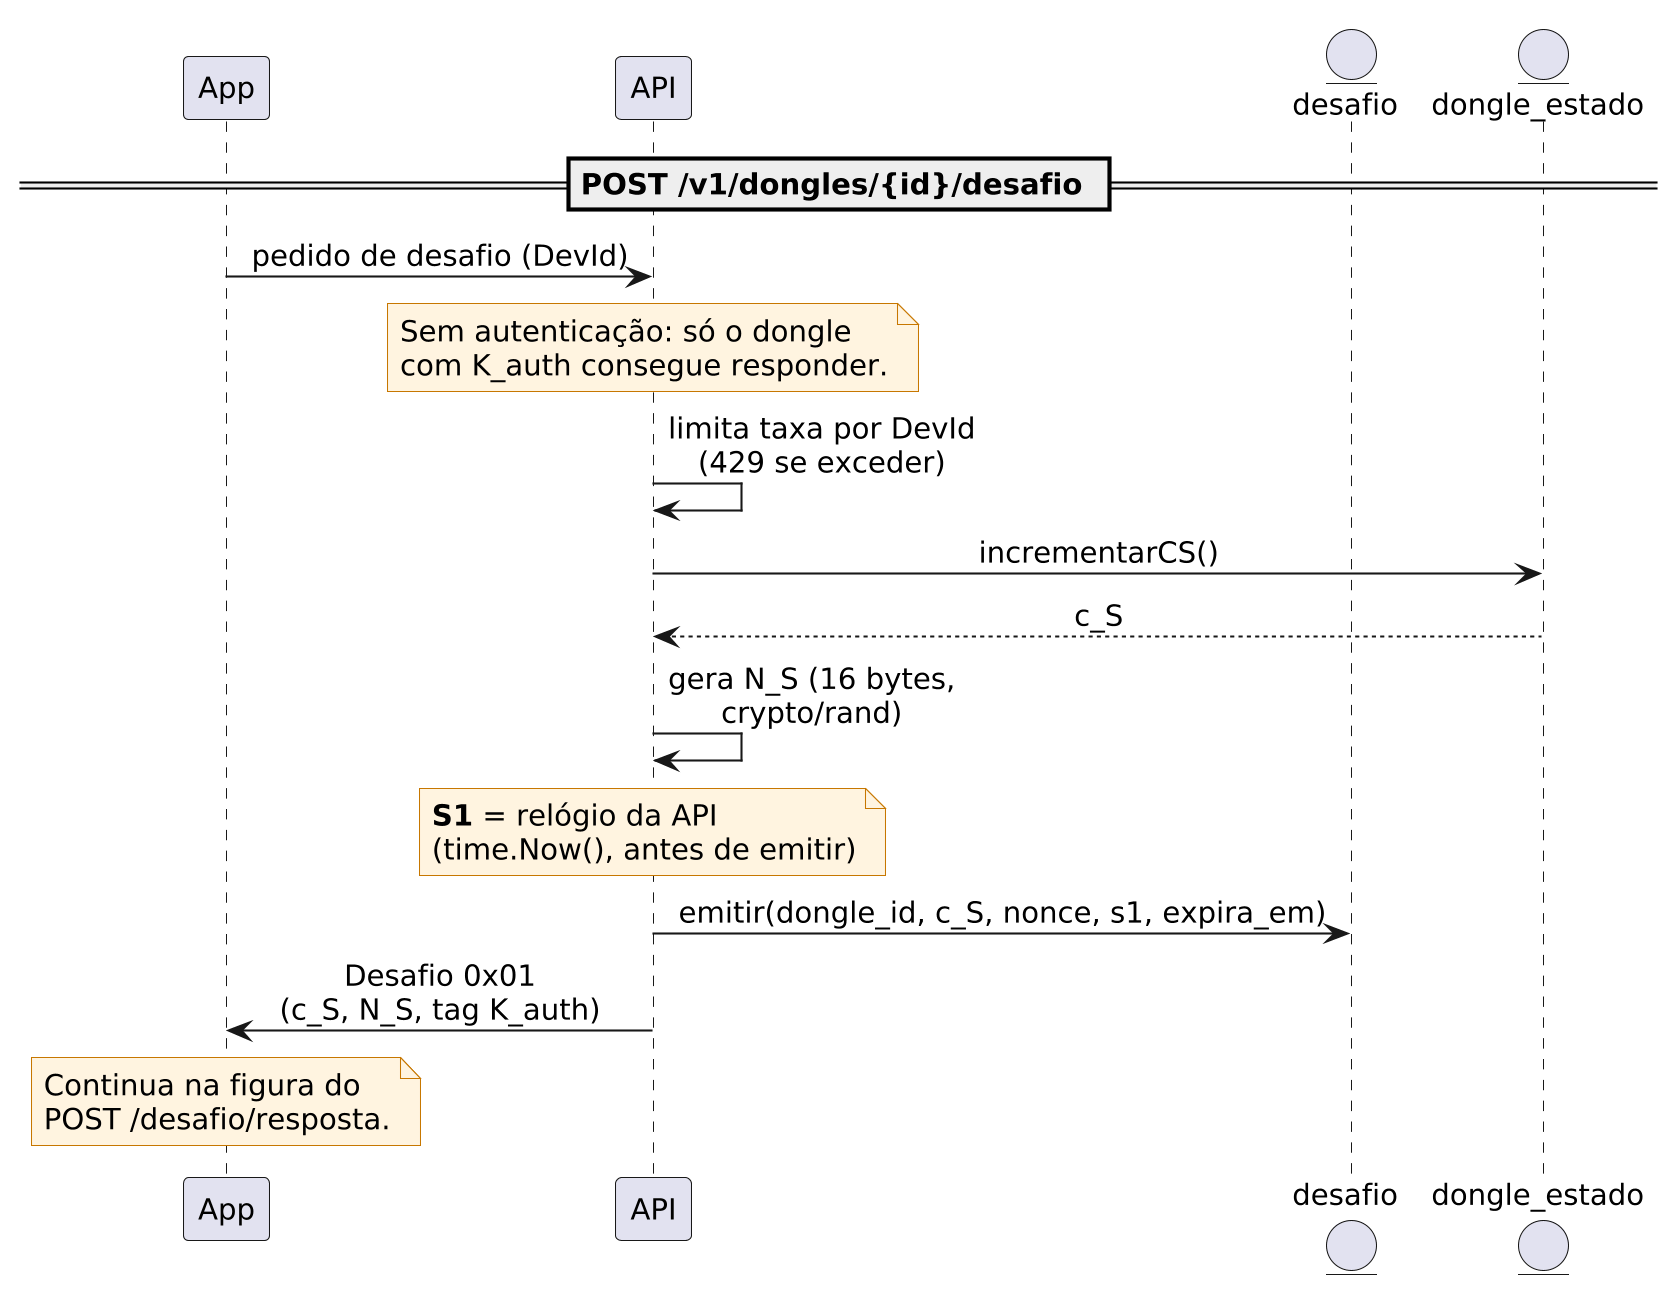
\includegraphics[width=0.85\textwidth]{../../assets/aux-docs/handshake-servidor-desafio.png}
	\legend{Fonte: elaborado pelo autor.}
\end{figure}

\begin{figure}[H]
	\centering
	\caption{Diagrama de sequência do \textit{handshake} no servidor: \texttt{POST /desafio/resposta}}
	\label{fig:handshake-servidor-resposta}
	% Fonte PlantUML: ../assets/aux-docs/plantuml/handshake-servidor-resposta.puml
	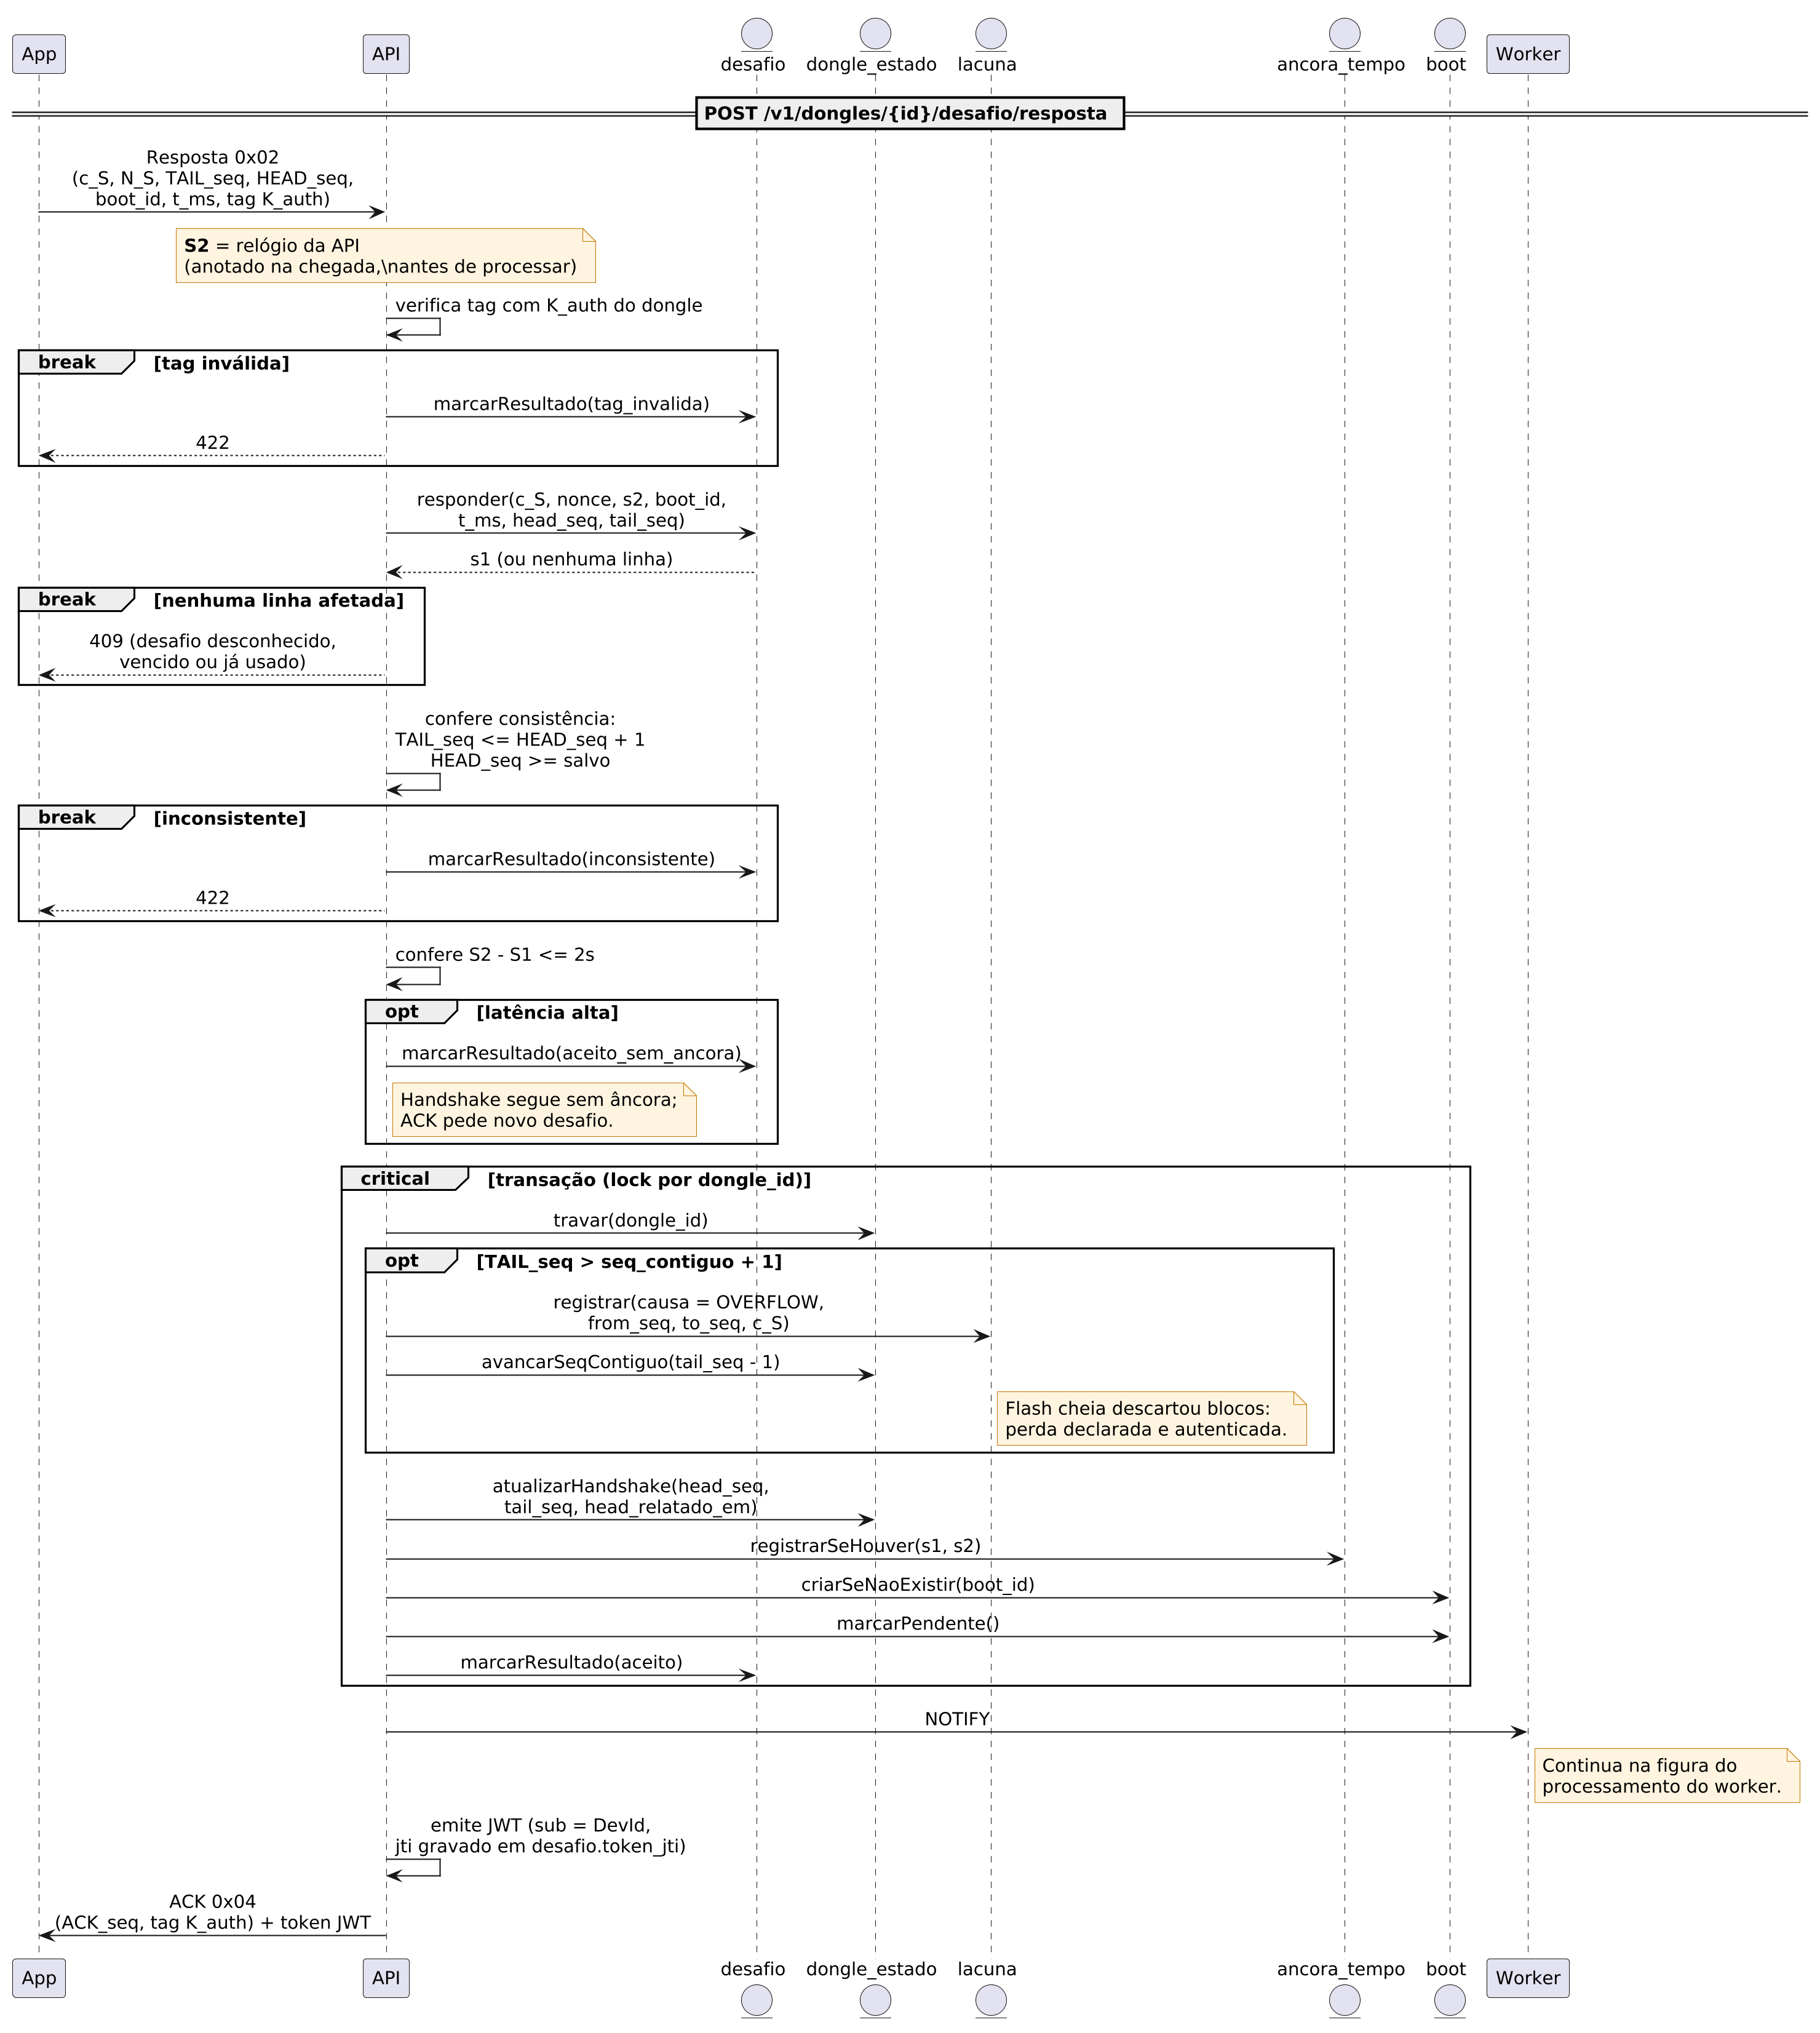
\includegraphics[width=\textwidth]{../../assets/aux-docs/handshake-servidor-resposta.png}
	\legend{Fonte: elaborado pelo autor.}
\end{figure}

\begin{figure}[H]
	\centering
	\caption{Diagrama de sequência do \textit{handshake} no servidor: processamento assíncrono do worker}
	\label{fig:handshake-servidor-worker}
	% Fonte PlantUML: ../assets/aux-docs/plantuml/handshake-servidor-worker.puml
	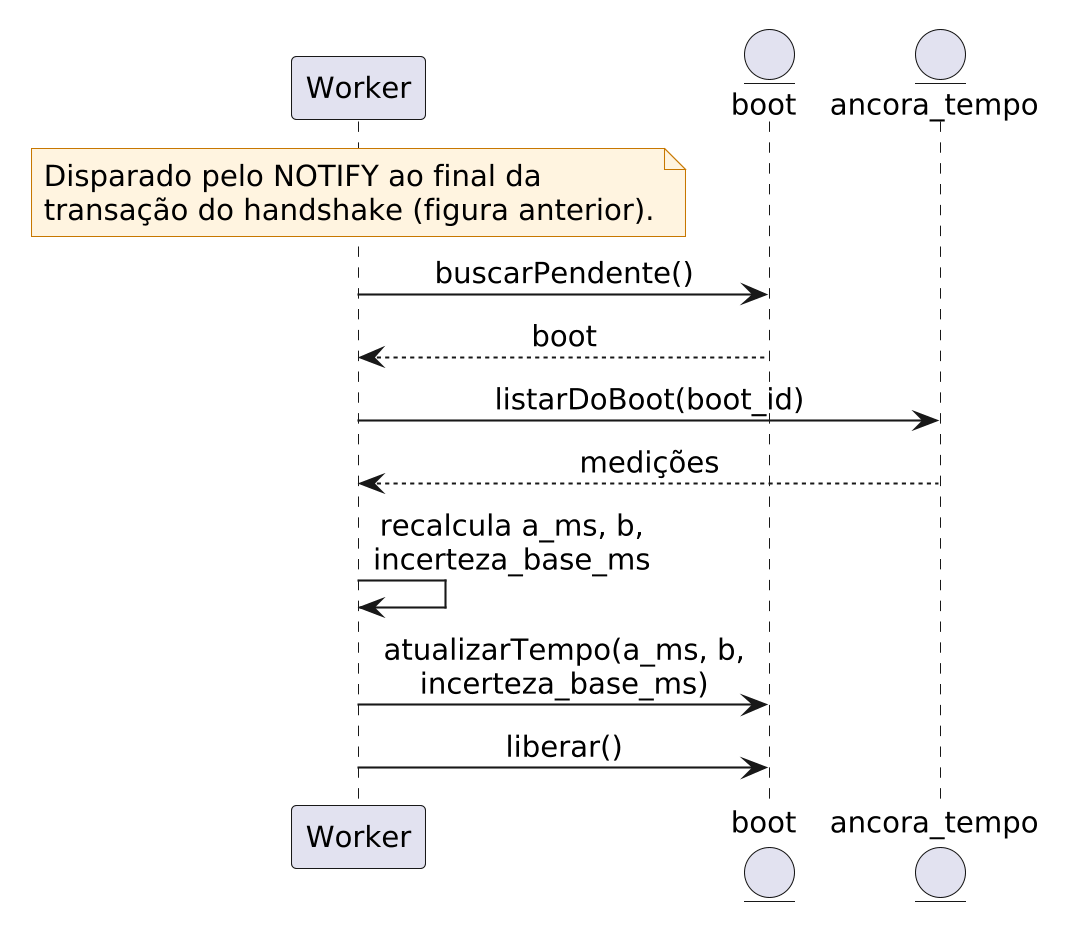
\includegraphics[width=0.6\textwidth]{../../assets/aux-docs/handshake-servidor-worker.png}
	\legend{Fonte: elaborado pelo autor.}
\end{figure}

%\subsection{Servidor de aplicação}

%\subsection{Servidor KMS}

\postextual

\bibliography{../abntex2-modelo-references}

\end{document}
